\documentclass[12pt, landscape]{article}
\usepackage[scaled=0.92]{helvet}
\usepackage{multicol}
\usepackage{calc}
\usepackage{ifthen}
\usepackage[landscape]{geometry}
%\usepackage{hyperref}

\usepackage{newtxtext} 

%for strikeout
\usepackage{ulem}

%For editing parbox
\usepackage[table]{xcolor}
%For editing itemise margins, reduce iterm separaion and list separation
\usepackage{enumitem}
% For math
\usepackage{amsmath,amsthm,amsfonts,amssymb}

%For pictures / figures
\usepackage{color,graphicx,overpic}
\graphicspath{ {./images/} }

%\usepackage{newtxtext} 
%\usepackage{amssymb}
%\usepackage[table]{xcolor}
%\usepackage{vwcol}
%\usepackage{tikz}
%\usepackage{wrapfig}
%\usepackage{makecell}


% For Code Blocks
\usepackage{xcolor}
\usepackage{listings}

\lstdefinestyle{mystyle}{
	backgroundcolor=\color{gray!25!white},
	basicstyle=\scriptsize,
	numbers=none,    %or = none or left
	showstringspaces=false,
	breaklines=true,
	breakatwhitespace=false,                  
	captionpos=b,                    
	keepspaces=true,                                 
	numbersep=5pt,                  
	showspaces=false,                
	showtabs=false,                  
	tabsize=2,
 }
%Helpful:
%[linewidth = 1.0 \linewidth]
%\lstinline{}
% use \code{} for \lstinline with colorbox.
\newcommand{\code}[1]{\colorbox{gray!25!}{\lstinline|#1|}}
\lstset{style=mystyle}

% Template: Cheatsheet with code enabled

%--------------------------- PACKAGES ABOVE --------------------------------------------------------------

\pdfinfo{
  /Title (Documentname.pdf)
  /Creator (Ger Teck)
  /Author (Ger Teck)
  /Subject ()
  /Keywords (tex)}

%% Margins for PAPER

% This sets page margins to .5 inch if using letter paper, and to 1cm
% if using A4 paper. (This probably isn't strictly necessary.)
% If using another size paper, use default 1cm margins.
\ifthenelse{\lengthtest { \paperwidth = 11in}}
	{ \geometry{top=.3in,left=.3in,right=.3in,bottom=.3in} }
	{\ifthenelse{ \lengthtest{ \paperwidth = 297mm}}
		{\geometry{top=1cm,left=1cm,right=1cm,bottom=1cm} }
		{\geometry{top=1cm,left=1cm,right=1cm,bottom=1cm} }
	}

% Turn off header and footer
\pagestyle{empty}

% for tight centres (less spacing)
\newenvironment{tightcenter}{%
  \setlength\topsep{0.5pt}
  \setlength\parskip{0.5pt}
  \begin{center}
}{%
  \end{center}
}

% Redefine section commands to use less space
\makeatletter
\renewcommand{\section}{\@startsection{section}{1}{0mm}%
                                {-1ex plus -.5ex minus -.2ex}%
                                {0.5ex plus .2ex}%x
                                {\normalfont\large\bfseries}}
\renewcommand{\subsection}{\@startsection{subsection}{2}{0.1mm}%
                                {-1explus -.5ex minus -.2ex}%
                                {0.5ex plus .2ex}%
                                {\normalfont\normalsize\bfseries}}
\renewcommand{\subsubsection}{\@startsection{subsubsection}{3}{0.1mm}%
                                {-1ex plus -.5ex minus -.2ex}%
                                {1ex plus .2ex}%
                                {\normalfont\small\bfseries}}
% change font
%\renewcommand{\familydefault}{\sfdefault}
%\renewcommand\rmdefault{\sfdefault}
\linespread{1.05}

\makeatother

% Define BibTeX command
\def\BibTeX{{\rm B\kern-.05em{\sc i\kern-.025em b}\kern-.08em
    T\kern-.1667em\lower.7ex\hbox{E}\kern-.125emX}}

% Don't print section numbers
\setcounter{secnumdepth}{0}

\setlength{\parindent}{0pt}
\setlength{\parskip}{0pt plus 0.5ex}

%% this changes all items (enumerate and itemize, reduce margins)
\setlength{\leftmargini}{0.5cm}
\setlength{\leftmarginii}{0.5cm}
\setlist[itemize,1]{leftmargin=2mm,labelindent=1mm,labelsep=1mm, itemsep = 1mm}
\setlist[itemize,2]{leftmargin=4mm,labelindent=1mm,labelsep=1mm, itemsep = 1mm}
\itemsep = 0mm
\setlist{nosep}

% Need Logo Picture
%Watermark Top Right
%\usepackage{atbegshi,picture}
%\AtBeginShipout{\AtBeginShipoutUpperLeft{%
 % \put(\dimexpr\paperwidth-1.2cm\relax, -1.2cm){\makebox[0pt][r]{\framebox{
\includegraphics[width = 0.3cm]{mountainbooks} Ger Teck}}}%
%}}


% -------------------------------------------------------------------------------

% START OF DOCUMENT HERE

\begin{document}
\raggedright
\footnotesize
\begin{multicols*}{3}



% multicol parameters
% These lengths are set only within the two main columns
%\setlength{\columnseprule}{0.25pt}
\setlength{\premulticols}{1pt}
\setlength{\postmulticols}{1pt}
\setlength{\multicolsep}{1pt}
\setlength{\columnsep}{2pt}

%% DOCUMENT NAME HERE
\begin{center}
     \Large{\textbf{CS2105 Comp. Networks Notes}} \\
\end{center}
AY23/24 Sem 1. github.com/gerteck
  
\section{1. Computer Networks Introduction}
\begin{itemize}
\item Fundamental concepts and principles behind computer networking, with internet as case study.
\item Connected by commmunication links and packet switches.
\end{itemize}

\subsubsection{Internet}
\begin{itemize}
\item The Internet is a network of connected computing devices (e.g. PC, server, laptop, smartphone). 
\item Such devices are known as hosts or end systems. Hosts run network applications (e.g. Tele, browser, Zoom)
\item Packet switching network, users' packets share network resources that are used on demand. Excessive congestion is possible.
\item \textbf{Network of networks} Hosts connect to Internet via access ISPs (Internet Service Providers), which themselves are interconnected. 
\centerline{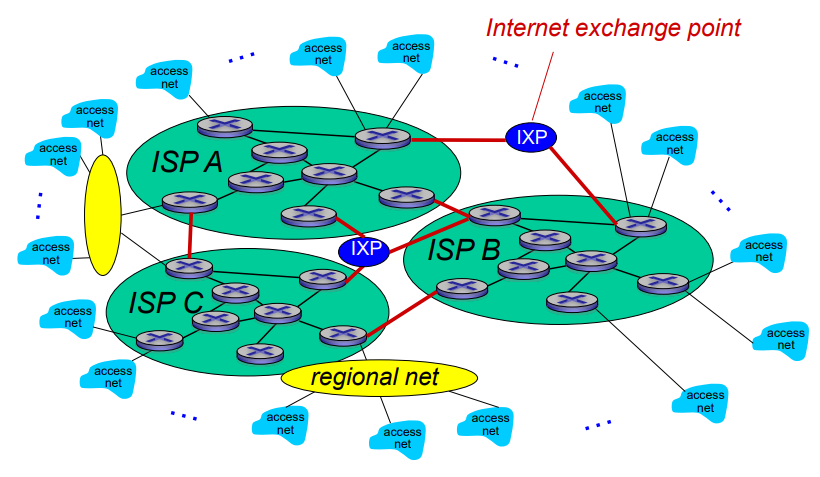
\includegraphics[width=0.6\linewidth]{internetstructure}}
\end{itemize}


\subsubsection{Network Edge (Access Network)}
\begin{itemize}
\item The access network is the network that physically
connects an end system to the first router on a path
from that end system to any distant end system.
\item E.g. Residential access networks, mobile access networks.
\end{itemize}
  
\subsubsection{Network Core}
\begin{itemize}
\item A mesh of interconnected routers.
\item Data is transmitted through network through:
\item \textbf{Circuit switching:} dedicated circuit per call
\item \textbf{Packet switching:} data sent through net in discrete “chunks"
\end{itemize}
  
\subsubsection{Circuit Switching}
\begin{itemize}
\item End-end resources are allocated to and reserved for “call”  between source \& dest:
\item call setup required, circuit-like (guaranteed) performance
\item circuit segment idle \textbf{silent periods} if not used by call (no sharing)
\item commonly used in traditional telephone network
\end{itemize}

\subsubsection{Packet Switching}
\begin{itemize}
\item Host sending function: breaks application message into smaller 
chunks, known as packets, of length $L$ bits. Then, transmits packets onto the link at transmission rate $R$.
\item Packets are passed from one router to the next, across links on path from source to destination.
\item link transmission rate is aka link capacity or \textbf{link bandwidth}
\item \textbf{Packet transmission delay} (time taken to transmit L-bit packet into Link) = $\frac{L}{R}$
\item \textbf{Store-and-forward}: entire packet must arrive at a router before it can be transmitted on the next link.
\end{itemize}


\subsubsection{Delay, Loss, Throughput}
Four sources of packet delay, suffered at each node, from source to destination. (\textbf{Total nodal delay})
\centerline{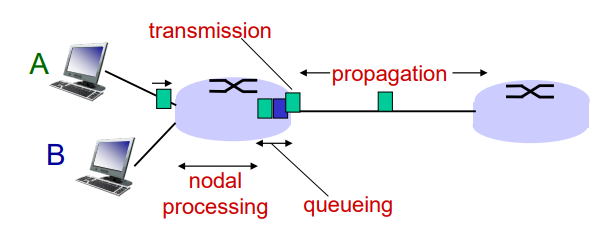
\includegraphics[width=0.6\linewidth]{totalnodaldelay}}
\begin{itemize}
\item \textbf{Nodal Processing Delay}: Time required to check for bit errors and determine output link. Typically $<$ msec.
\item \textbf{Queueing Delay}: Time waiting in queue for transmission, depends on earlier arrived packets. Typically $<$ msec. Additionally, possibility of
						packet loss if router queue full (buffer has reached finite capacity), and drops packet.
\item \textbf{Transmission Delay}: Time to push (last bit) of packet on wire. $d_{trans} = \frac{L}{R}$.
\item \textbf{Propagation Delay}: Time to propagate to next router. $d_{prop} = \frac{d}{s}$, where $d$ is length of physical link, $s$ propagation speed.
\item End to end packet delay is total time taken for packet to travel from source to destination, consisting of the 4 delays.
\item \textbf{Throughput}: How many bits can be transmitted per unit time, usually measured for end-to-end communication (as opposed to bandwidth for specific link).
\end{itemize}

\subsubsection{Internet Protocol Stack}
Protcols logically organised into 5 "layers" according to purpose. (Additionally presentation and session layers not included)
\begin{itemize}
\item \textbf{Application}: Where network applications and app-layer protocols reside. Packet here called message. \\ 
Examples: HTTP, SMTP, FTP
\item \textbf{Transport}: Transports app-layer messages between application endpoints. Packet here called segment.  \\
Examples: TCP, UDP
\item \textbf{Network}: Moves packets (datagrams) from one host to another. Includes IP protocol and other routing protocols.
\item \textbf{Link}: Moves packet from one node to another. Packet here called frame. \\
Example: Ethernet, WiFi
\item \textbf{Physical}: Moves individual bits within link-layer frame from one node to another. Link and transmission medium dependent.
\end{itemize}

\vfill \null
\columnbreak
%                              -----------------------------------------------------

\section{2. Application Layer}
\subsubsection{Principles of Network Applications}
\begin{itemize}
\item \textbf{Client-Server}: \\
• Server waits for incoming requests and provides required services to client. Easy scalability. \\
• Client initiates contact with server and requests service.
\item \textbf{Peer-To-Peer (P2P)}: \\
• No dedicated server, instead it relies on direct communication between pairs of intermittently connected hosts called peers. \\
• Self-scalability, each peer generates workload but adds service capacity by distributing files.
\end{itemize}

\subsubsection{Process Communication}
\begin{itemize}
\item \textbf{Socket}: A software interface that process uses to send messages and receive messages from network. Generally a combination of IP address and port number. 
\item \textbf{IP Address}: A 32-bit quantity, uniquely identifies host.
\item \textbf{Port Number}: A 16-bit integer used to identify a receiving process running in a host.
\end{itemize}

\subsubsection{Requirements of Transport Service}
\begin{itemize}
\item \textbf{Reliable Data Transfer}: Data to sent correctly and completely vs. loss-tolerant.
\item \textbf{Throughput}: Bandwidth-sensitive apps may need guaranteed throughput of r bits/sec. 
\item \textbf{Timing/Delay}: Real-time applications generally require low delays to be effective.
\item \textbf{Security}: Encryption, data integrity, authentication.
\end{itemize}

\subsubsection{Transport Layer Protocols}
Two main protocols for the Internet. \\
\begin{itemize}
\item \textbf{Transmission Control Protocol (TCP)} \\
• Reliable data transfer, Connection-oriented service: A handshake required.\\
• Flow control, Congestion control: Throttle sender when network overloaded \\
• Security: Can be enhanced at the app layer with Secure Sockets Layer \\
• Does not provide: Timing and throughput guarantee
\item \textbf{User Datagram Protocol (UDP)} \\
• Unreliable data transfer \\
• Connectionless: No handshake \\
• No flow control, no congestion control \\
• Does not provide: Timing and throughput guarantee, security.
\end{itemize}

\subsubsection{Application-Layer Protocols} 
An application-layer protocol defines:
\begin{itemize}
\item Types of messages exchanged, e.g. request and response messages.
\item Syntax of message types, e.g. fields and how they are delineated.
\item Semantics of the fields, i.e. what the information means.
\item Rules for when and how to send a message and respond to messages.
\end{itemize}

\subsection{Web \& HTTP}
\begin{itemize}
\item \textbf{Webpage}: Consists of base HTML files and referenced objects. Addressable by URL.
\item URL made up of hostname as well as path name. (E.g. http://www.comp.nus.edu.sg/~cs2105/img/doge.jpg)
\item \textbf{HyperText Transfer Protocol} is Web’s app-layer protocol.
\item \textbf{Client-server model:} Client requests, receives and displays Web objects, server is Web server that sends objects in response.
\item \textbf{Stateless}: server maintains no information about clients, and \textbf{Reliable}: Over TCP.
\item \textbf{Three-way Handshake}: Client sends small TCP segment to ask for connection, server acknowledges and responds, client acknowledges and sends it back with request message.
\end{itemize}

\subsubsection{HTTP versions}
\begin{itemize}
\item \textbf{RTT}: Round trip time, time taken for packet to travel from server and back to client, does not include transmission delay.
\item \textbf{Non-persistent HTTP}: Response time = $2 *$ RTT$+$ file transmission time (per object)
\item \textbf{Persistent HTTP}: Server leaves connection open after sending response, subsequent HTTP sent over same TCP connection. Also uses pipelining, send requests back to back.
\end{itemize}
\smallskip
\centerline{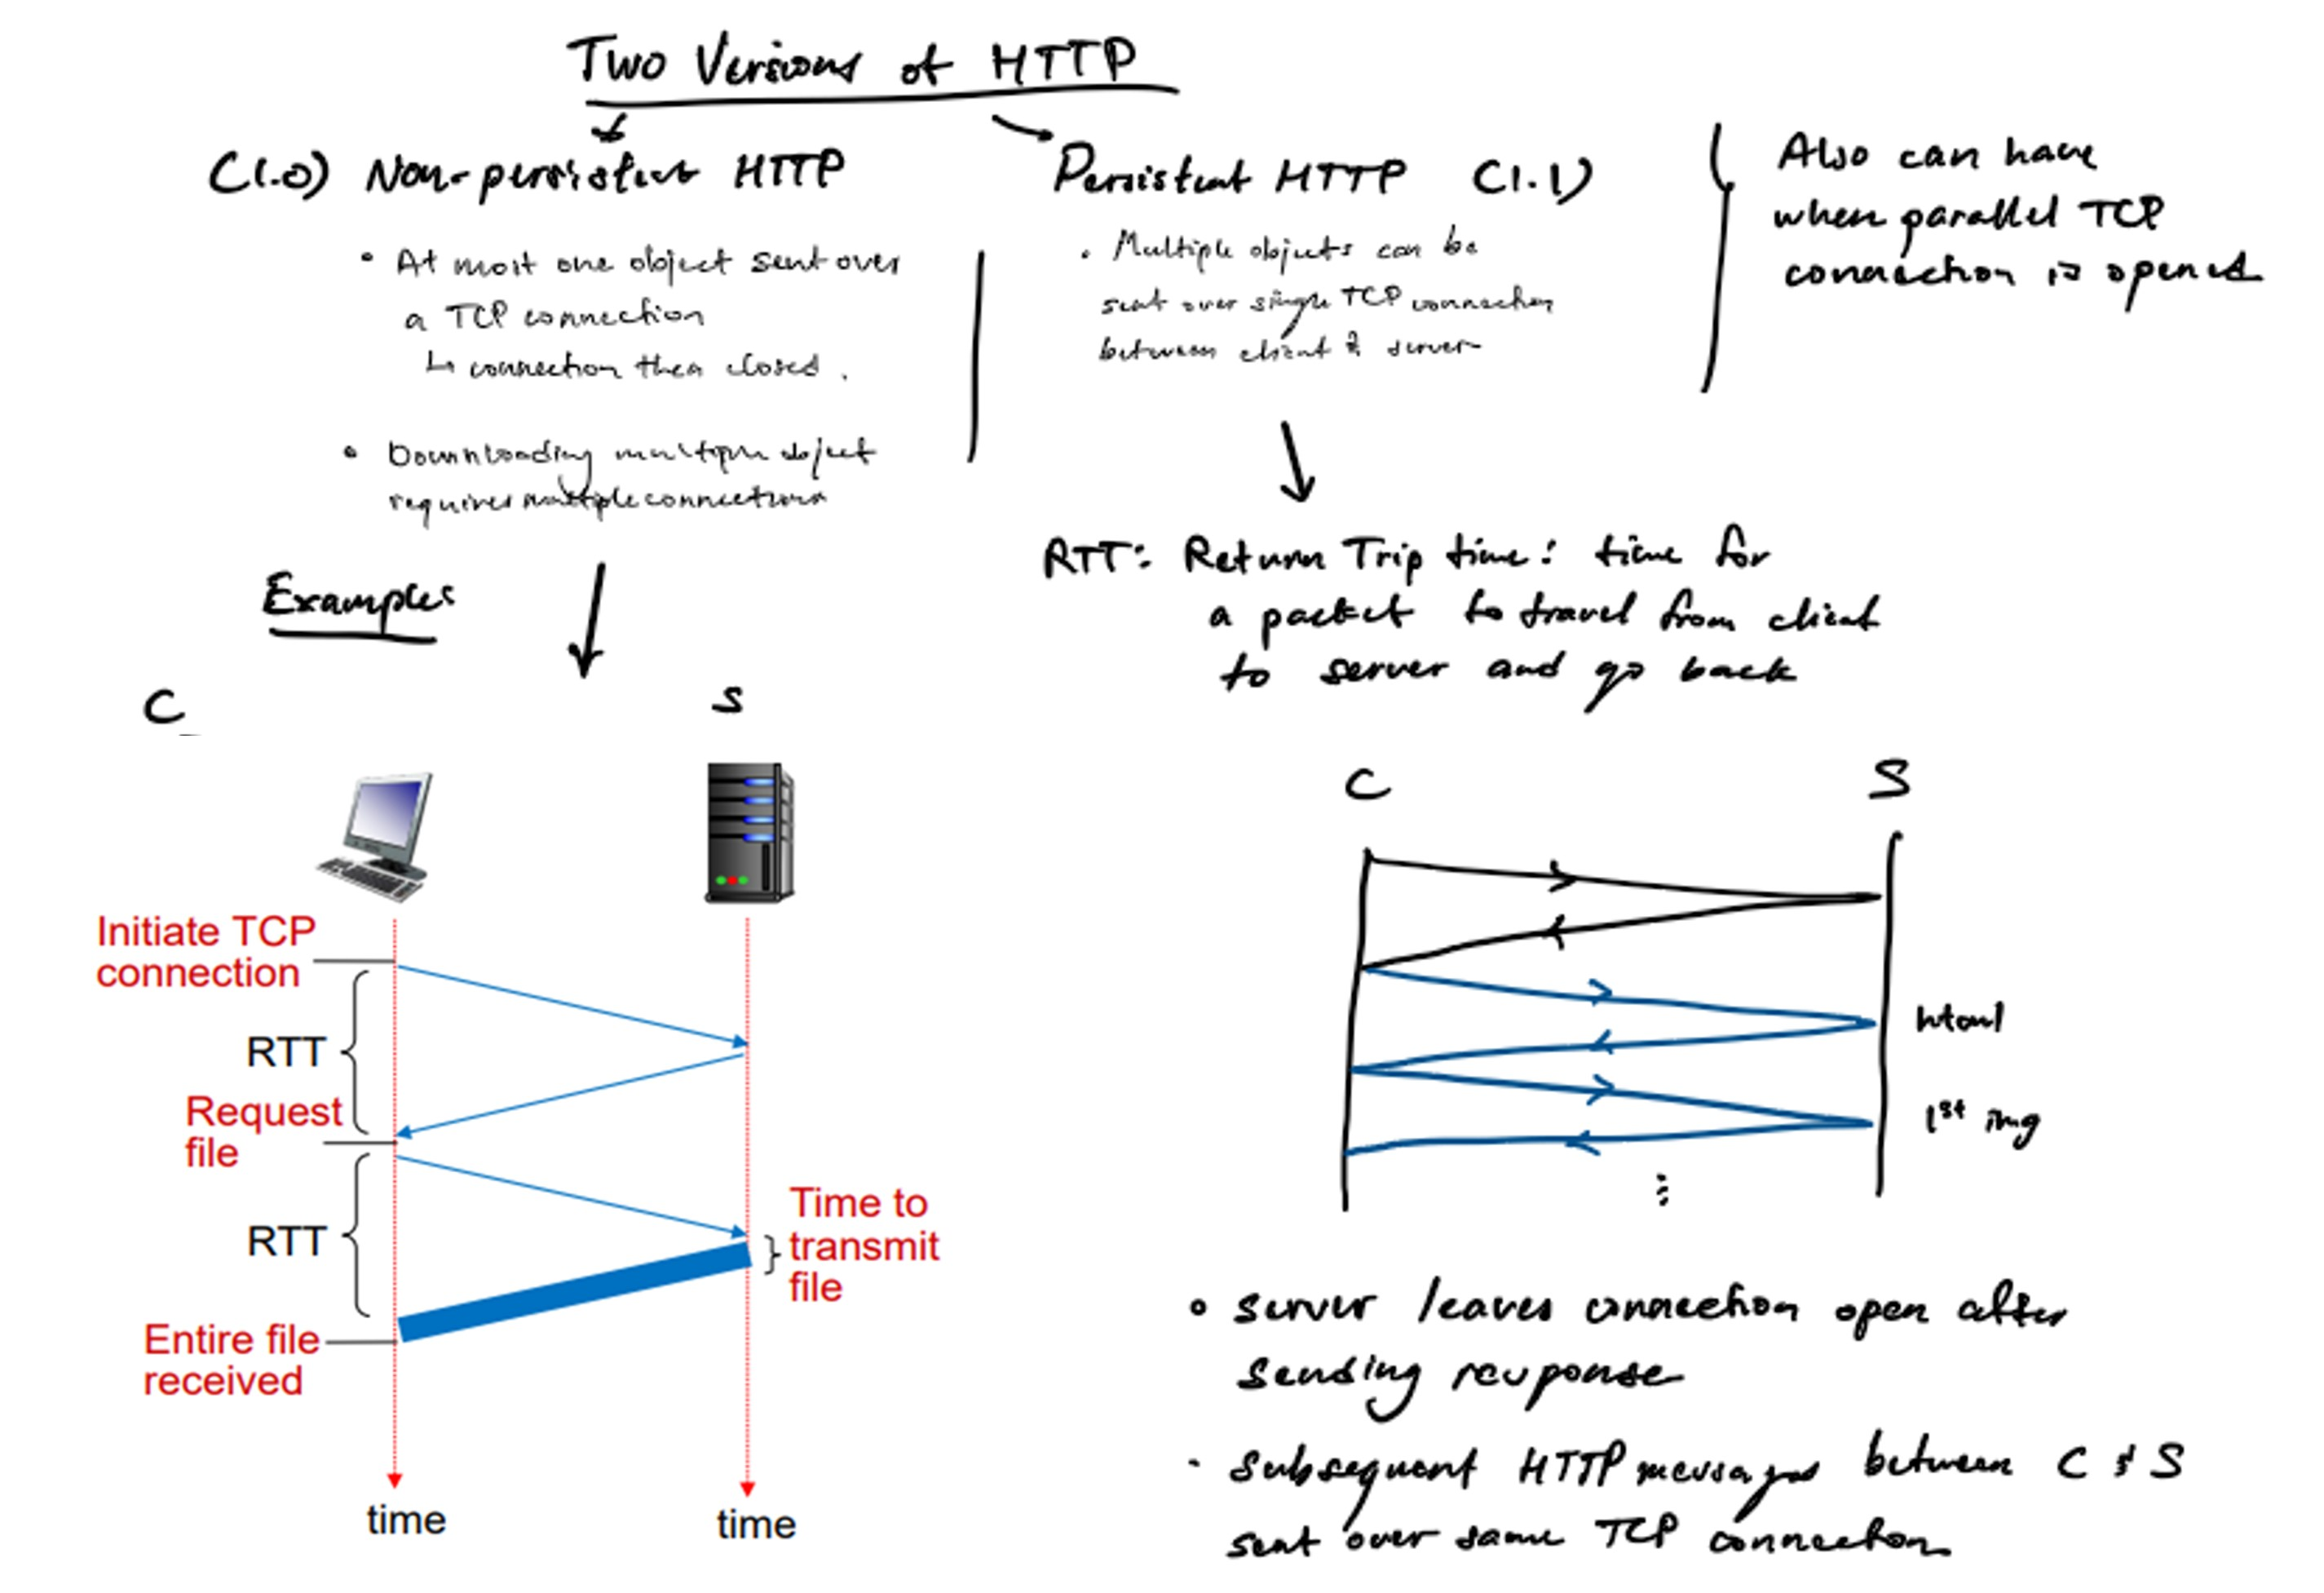
\includegraphics[width=1\linewidth]{HTTPmodes}}
\medskip
\subsubsection{HTTP Request}
\centerline{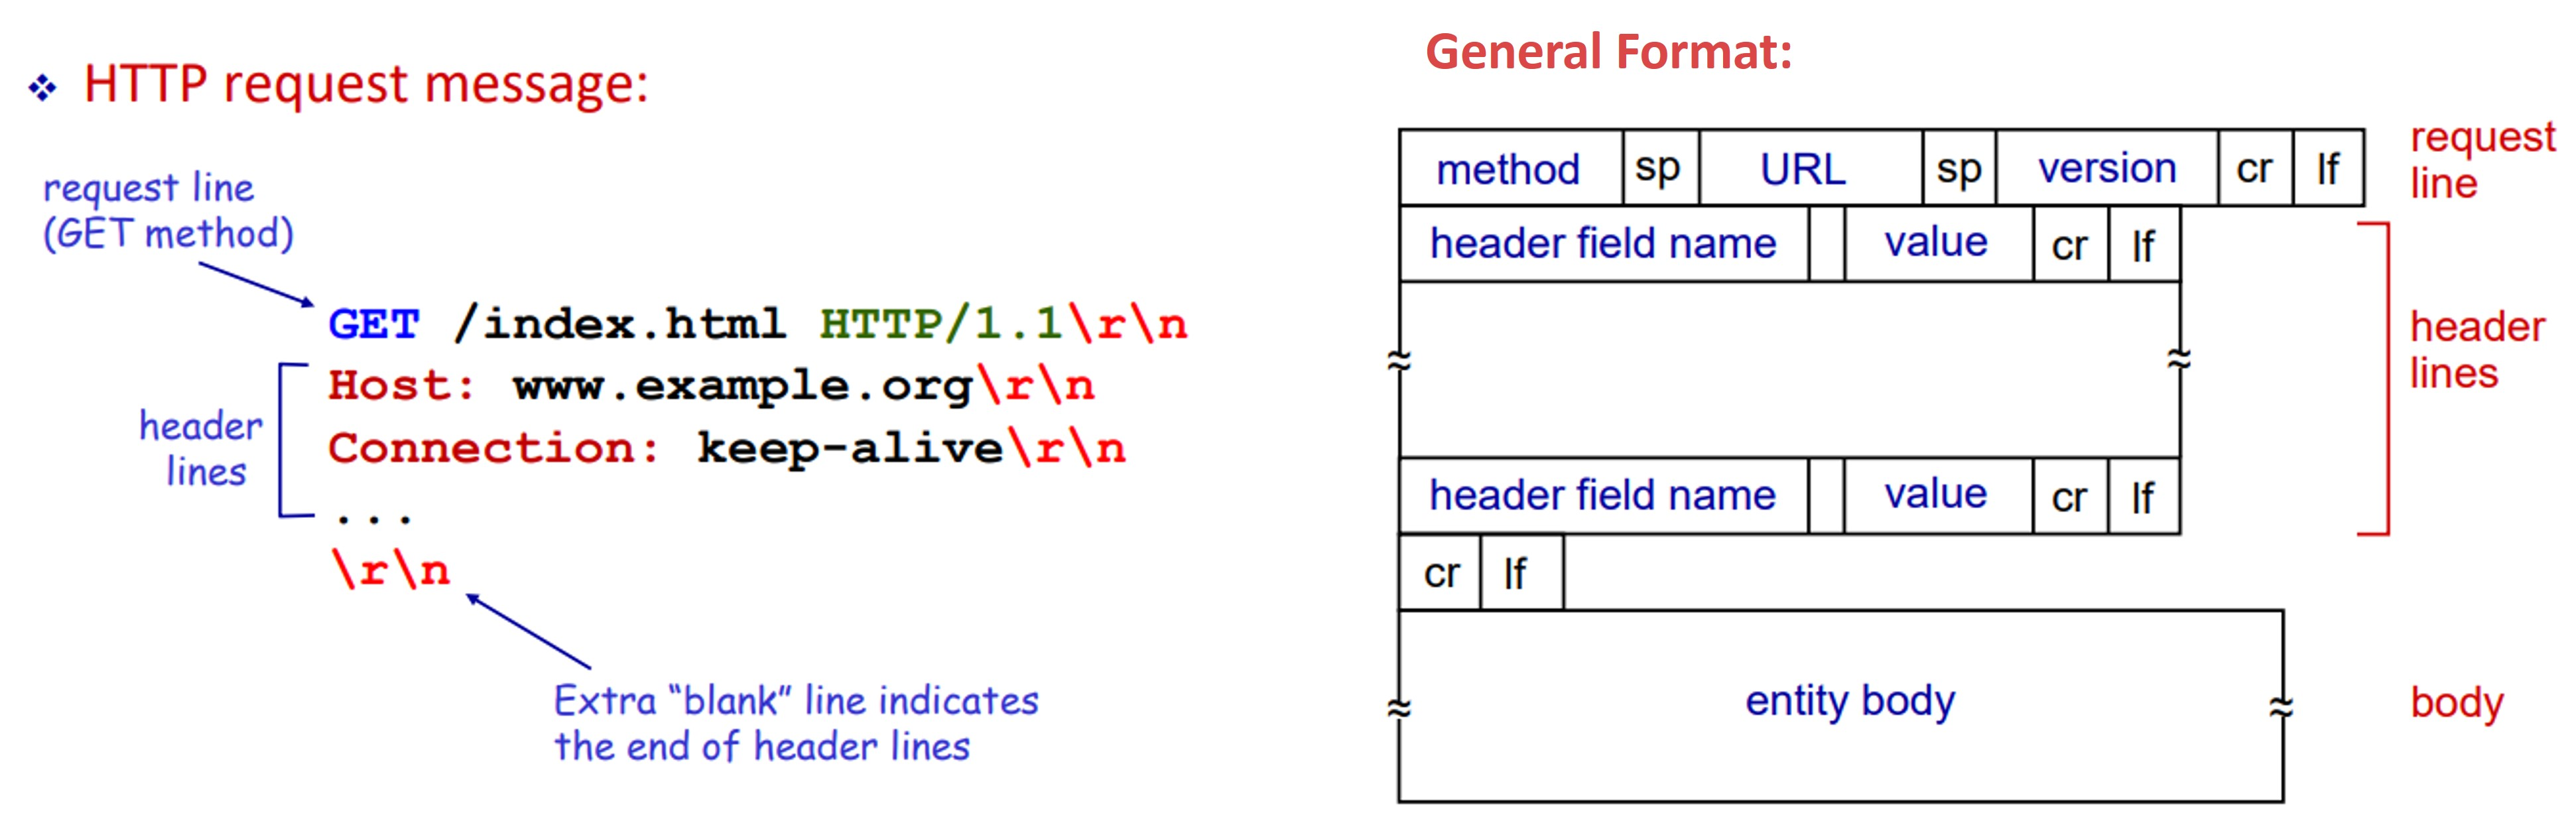
\includegraphics[width=1\linewidth]{HTTPrequest}}
\begin{itemize}
\item \textbf{HTTP 1.0 Methods}: GET (gets object), POST (posts form data), HEAD (gets header without body).
\item \textbf{HTTP 1.1 Methods}: GET, POST, HEAD, PUT (uploads file to path specified), DELETE
\end{itemize}
\medskip
\subsubsection{HTTP Response}
\centerline{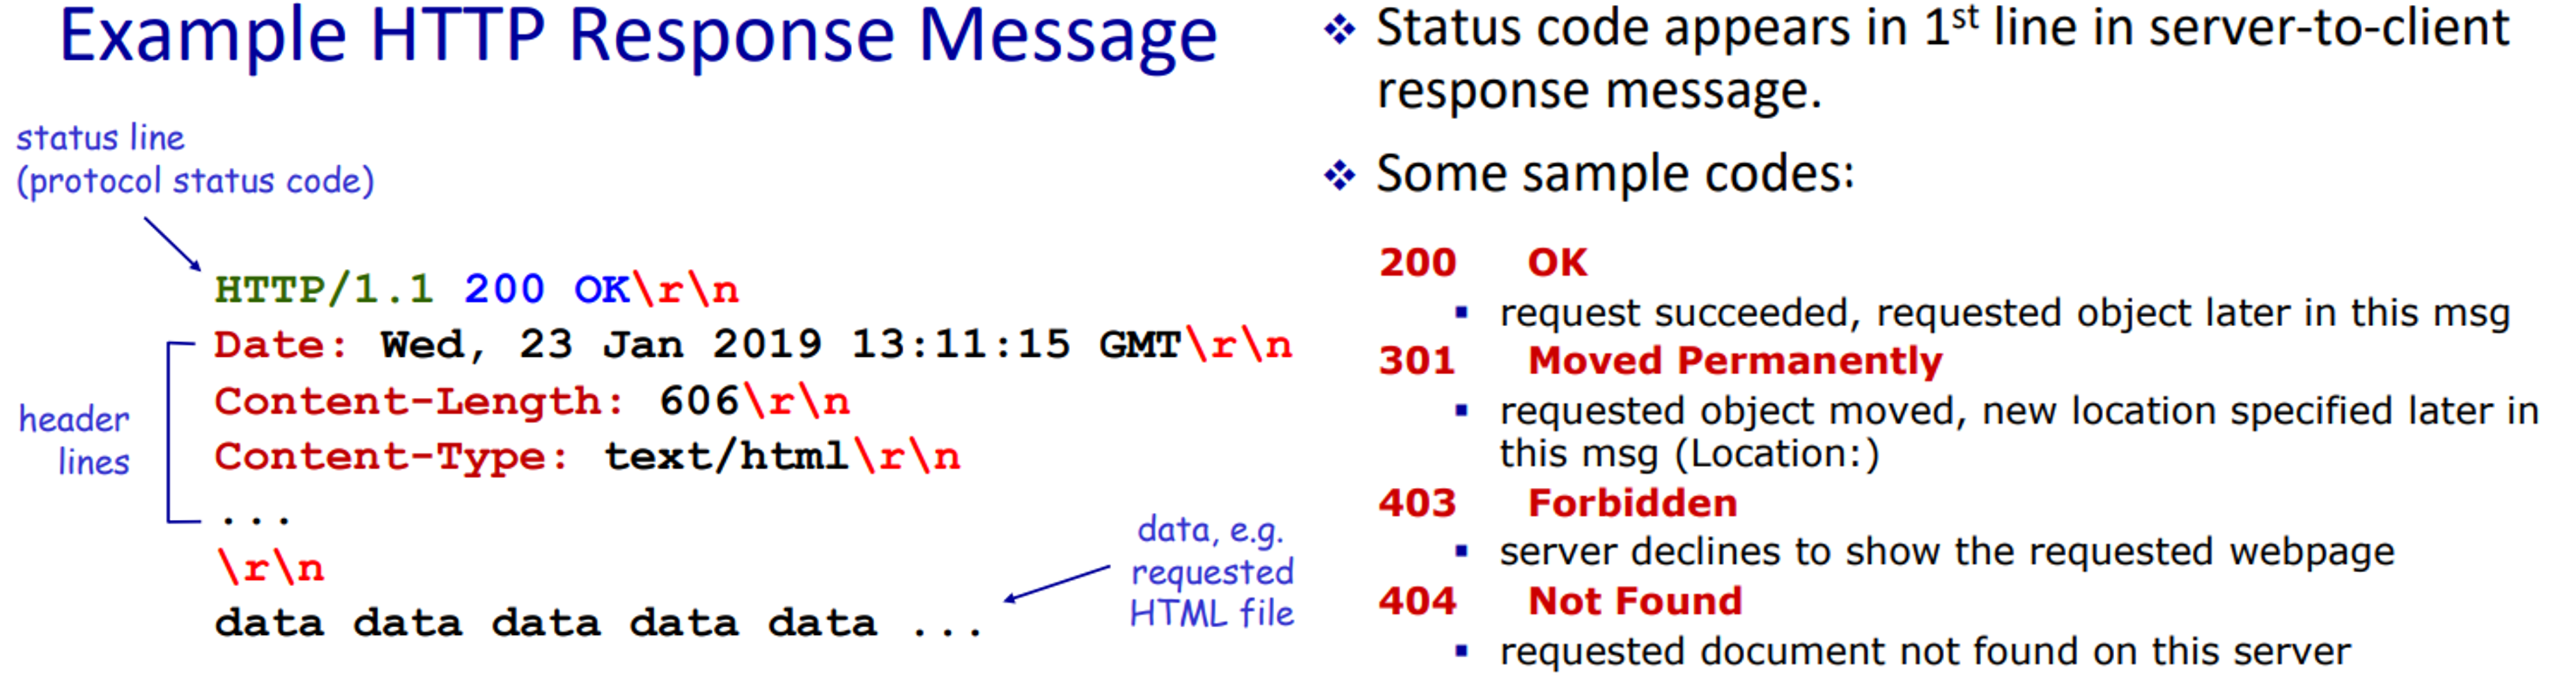
\includegraphics[width=1\linewidth]{HTTPresponse}}

\vfill \null
\columnbreak

\subsubsection{Cookies}
\begin{itemize}
\item HTTP is designed to be “stateless”, server maintains no information about past client requests. 
\item Good to maintain states over multiple transactions, e.g. shopping carts
\item \textbf{Cookie}: http messages carry “state”: \\
1) cookie header field of HTTP req/res messages \\ 
2) cookie file kept on user host, managed by browser\\
3) back-end database at Web site
\item \textbf{Conditional GET}: In cache, specify date of cached copy in HTTP request. Server response contains no object if cached copy is up to date.
\end{itemize}
\medskip
\centerline{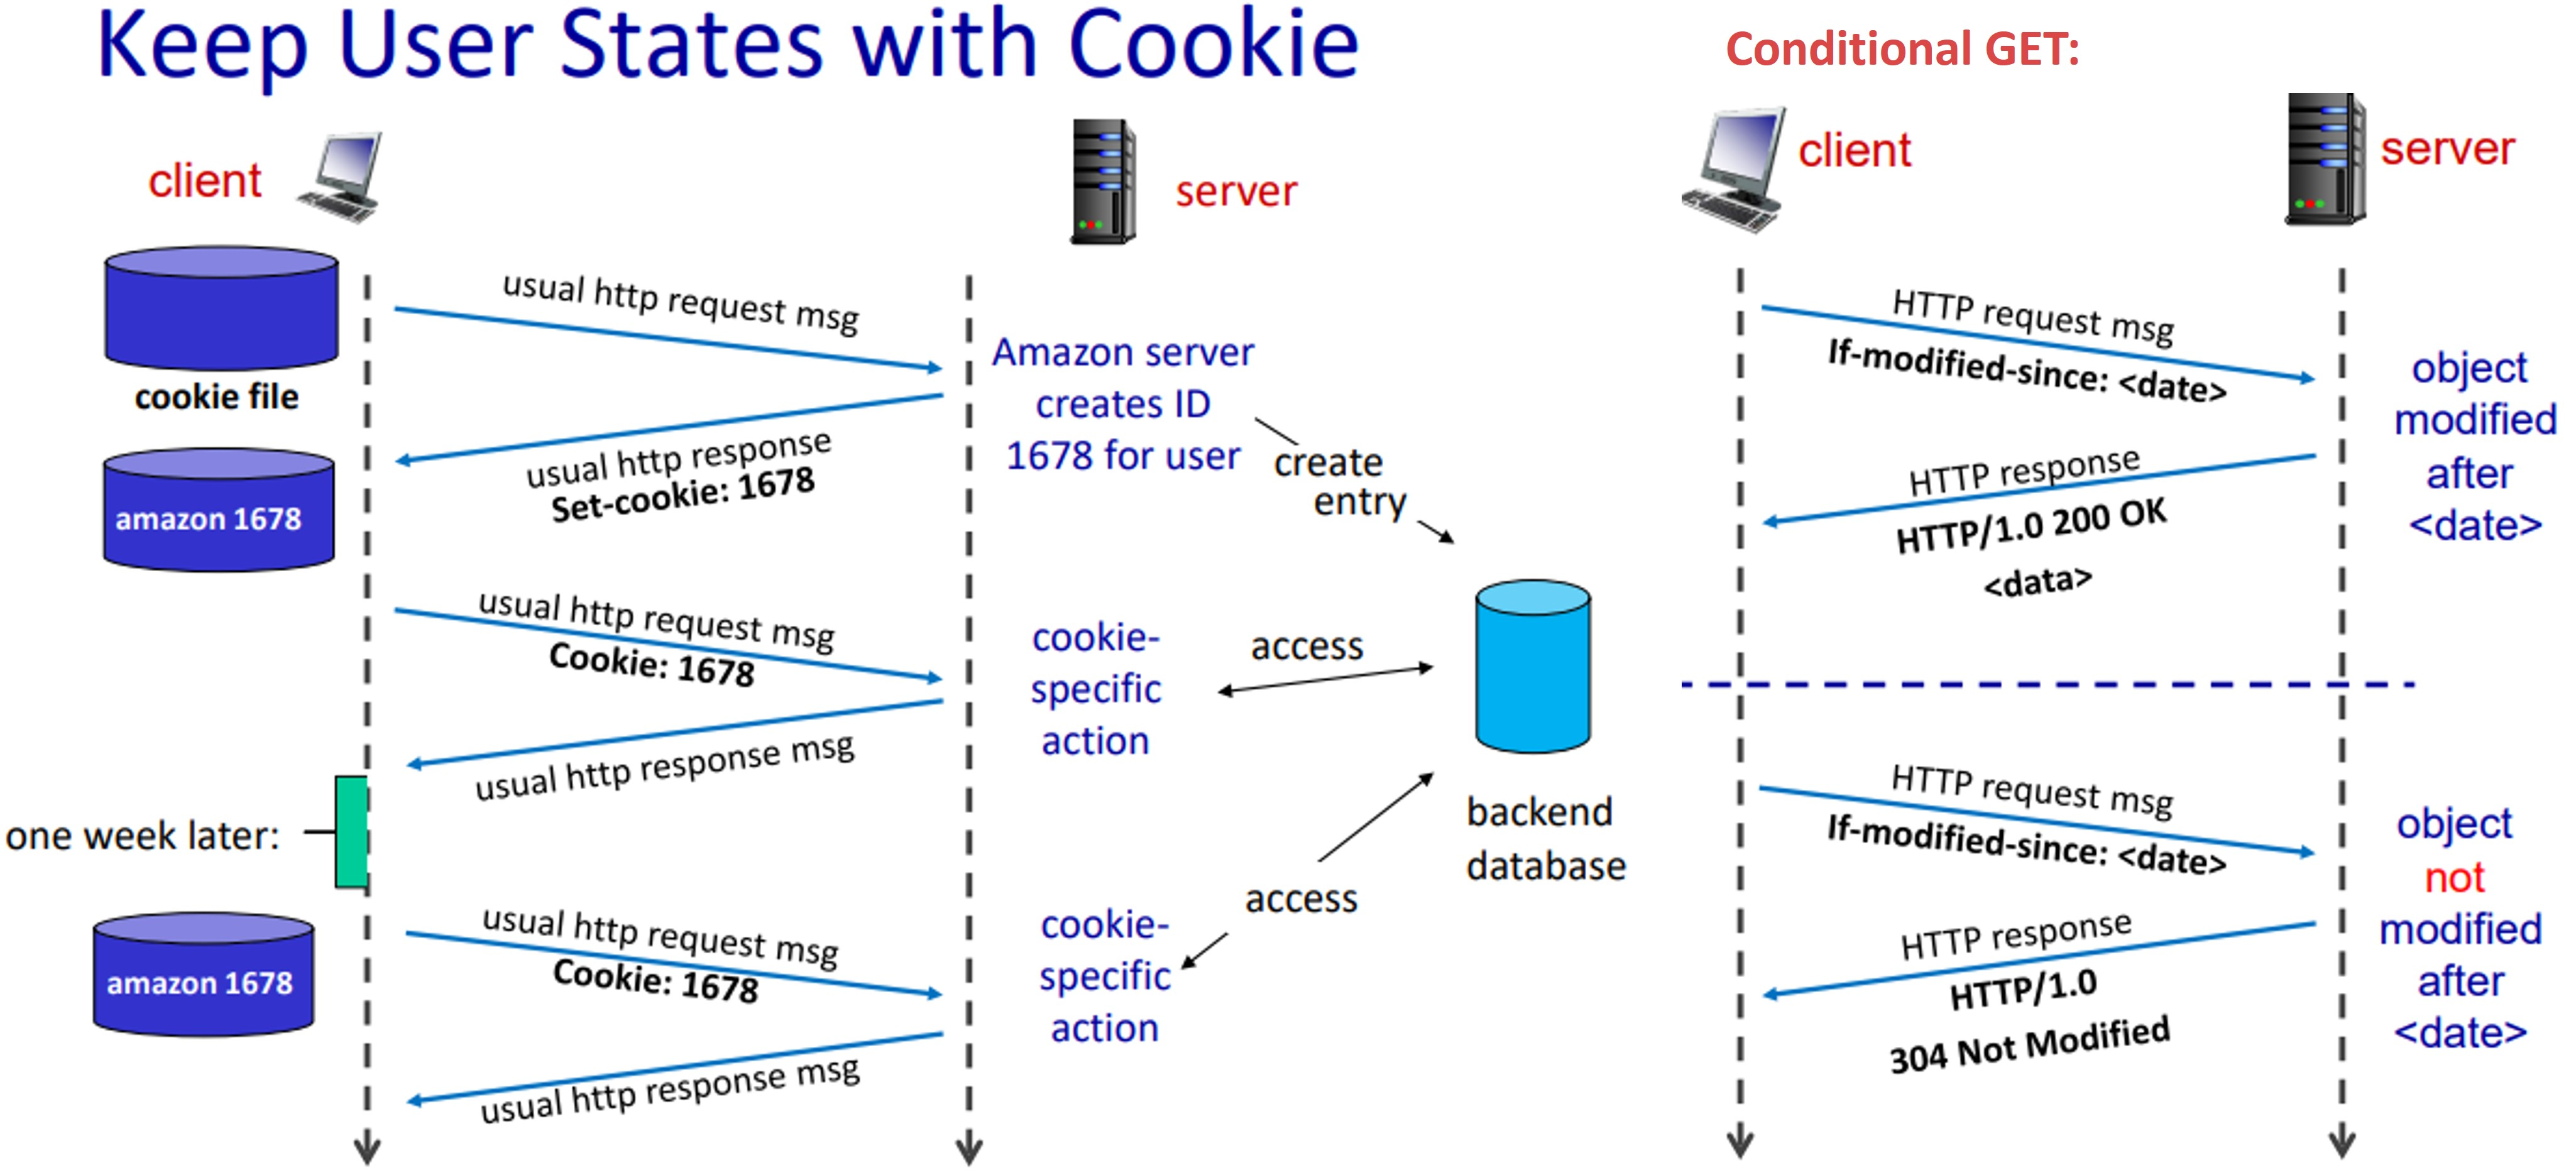
\includegraphics[width=1\linewidth]{HTTPcookies}}


\subsubsection{Domain Name System}
DNS translates between hostname and IP addresses. Client must carry out a DNS query to determine the 
IP address corresponding to the server name.
\begin{itemize}
\item \textbf{DNS: Resource Records (RR)}
\centerline{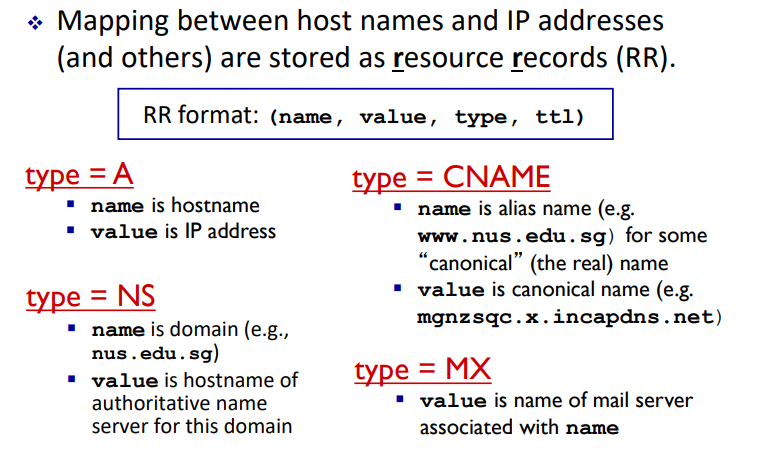
\includegraphics[width=1\linewidth]{DNSrr}}
\item \textbf{Distributed, Hierarchical Database}: DNS servers form hierarchy to distribute mappings. Contains root servers (for Top Level Domain TLD servers), 
								TLD servers (e.g. uk, sg), Authoritative servers.
\item Local DNS servers have local cache, acts as proxy, forward query into hierarchy if answer not found locally.
\item \textbf{DNS Caching}: Cache mapping, which expires after some time (TTL: time to live). 
\item DNS runs over \textbf{UDP}.
\end{itemize}

\subsubsection{DNS Name Resolution}
\centerline{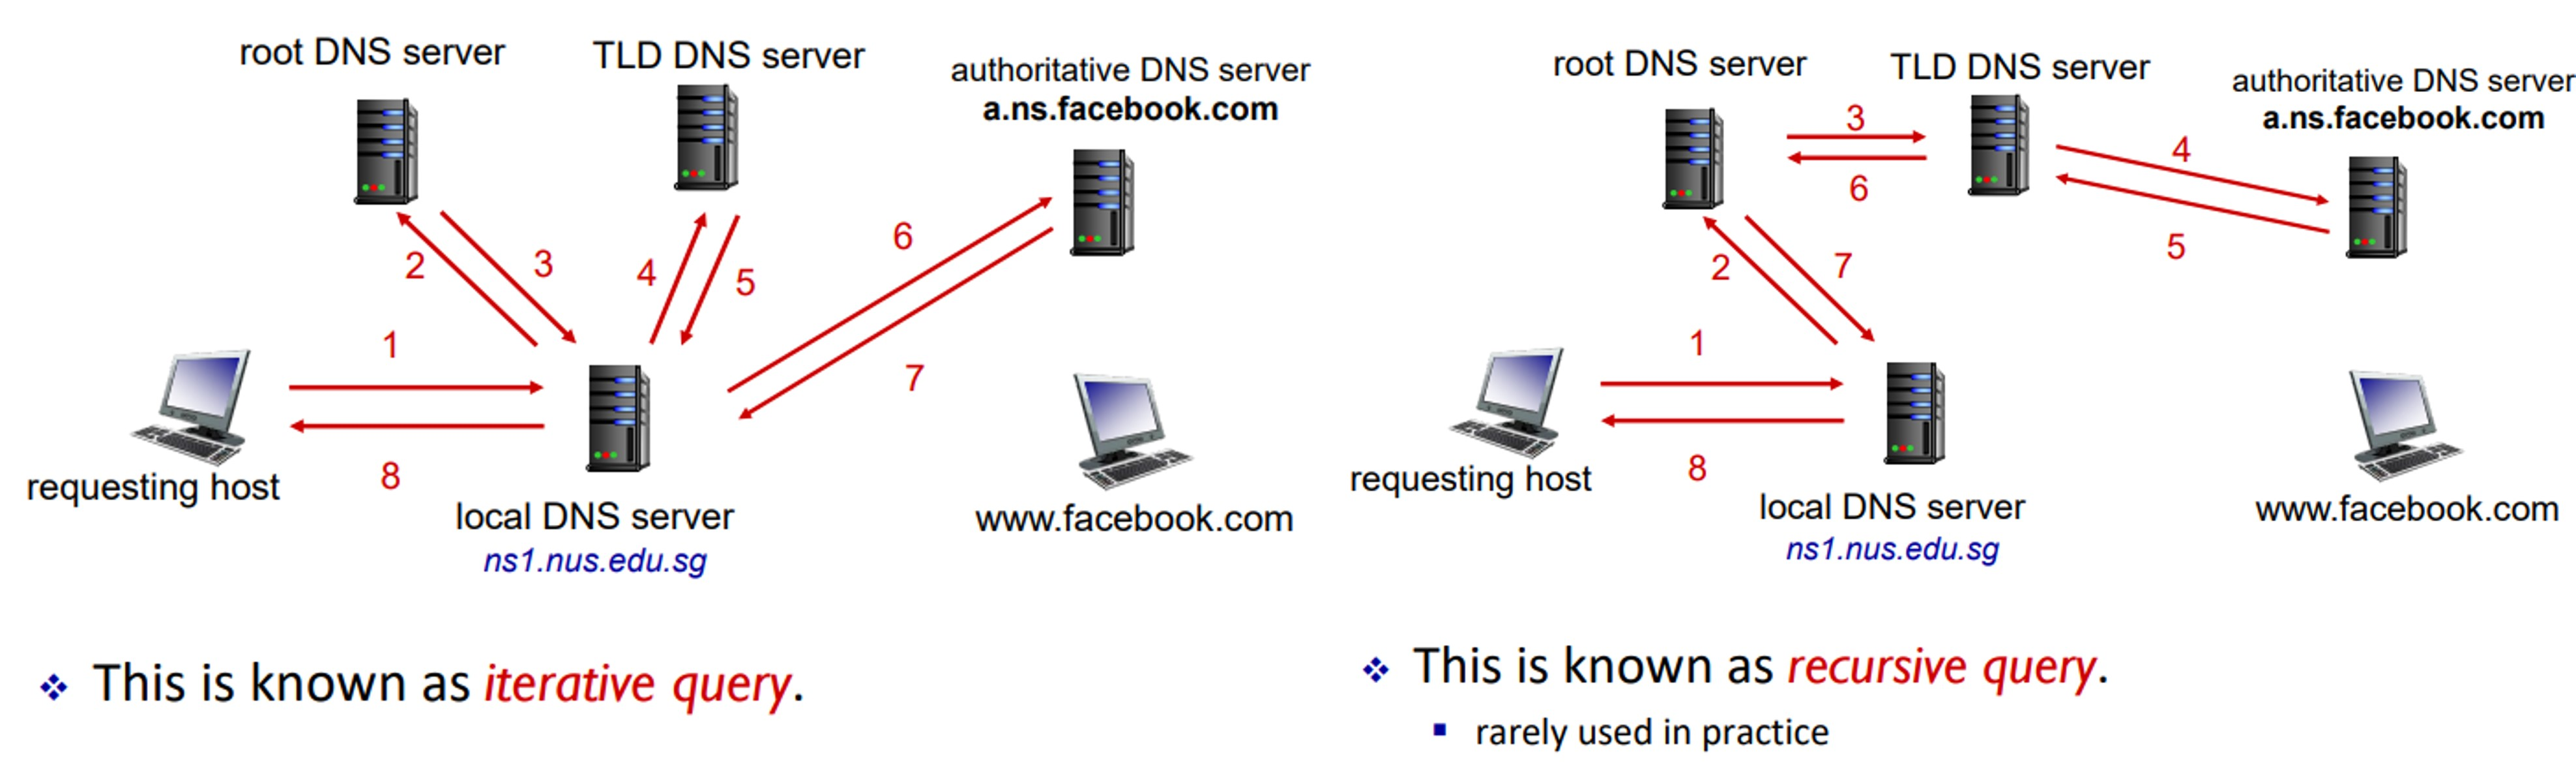
\includegraphics[width=1\linewidth]{DNSname}}
\medskip

\subsection{Socket Programming}
Applications treat the Internet as black box, send/receive message through sockets.
\begin{itemize}
\item Two types of sockets
\item \textbf{TCP}: reliable, byte stream-oriented socket
\item \textbf{UDP}: unreliable datagram socket
\end{itemize}

\subsubsection{UDP vs. TCP Socket}
\begin{itemize}
\item \textbf{UDP Socket:}Sender attach des IP address + port no. to each packet. (OS inserts add. info source IP and port). 
Receiver extracts sender IP + port number from packet.
\item \textbf{TCP Socket:} Attempts to establish TCP connection to server first. Server TCP contacted creates new socket to communicate with client, allows server to talk with multiple clients individually.
\end{itemize}
\centerline{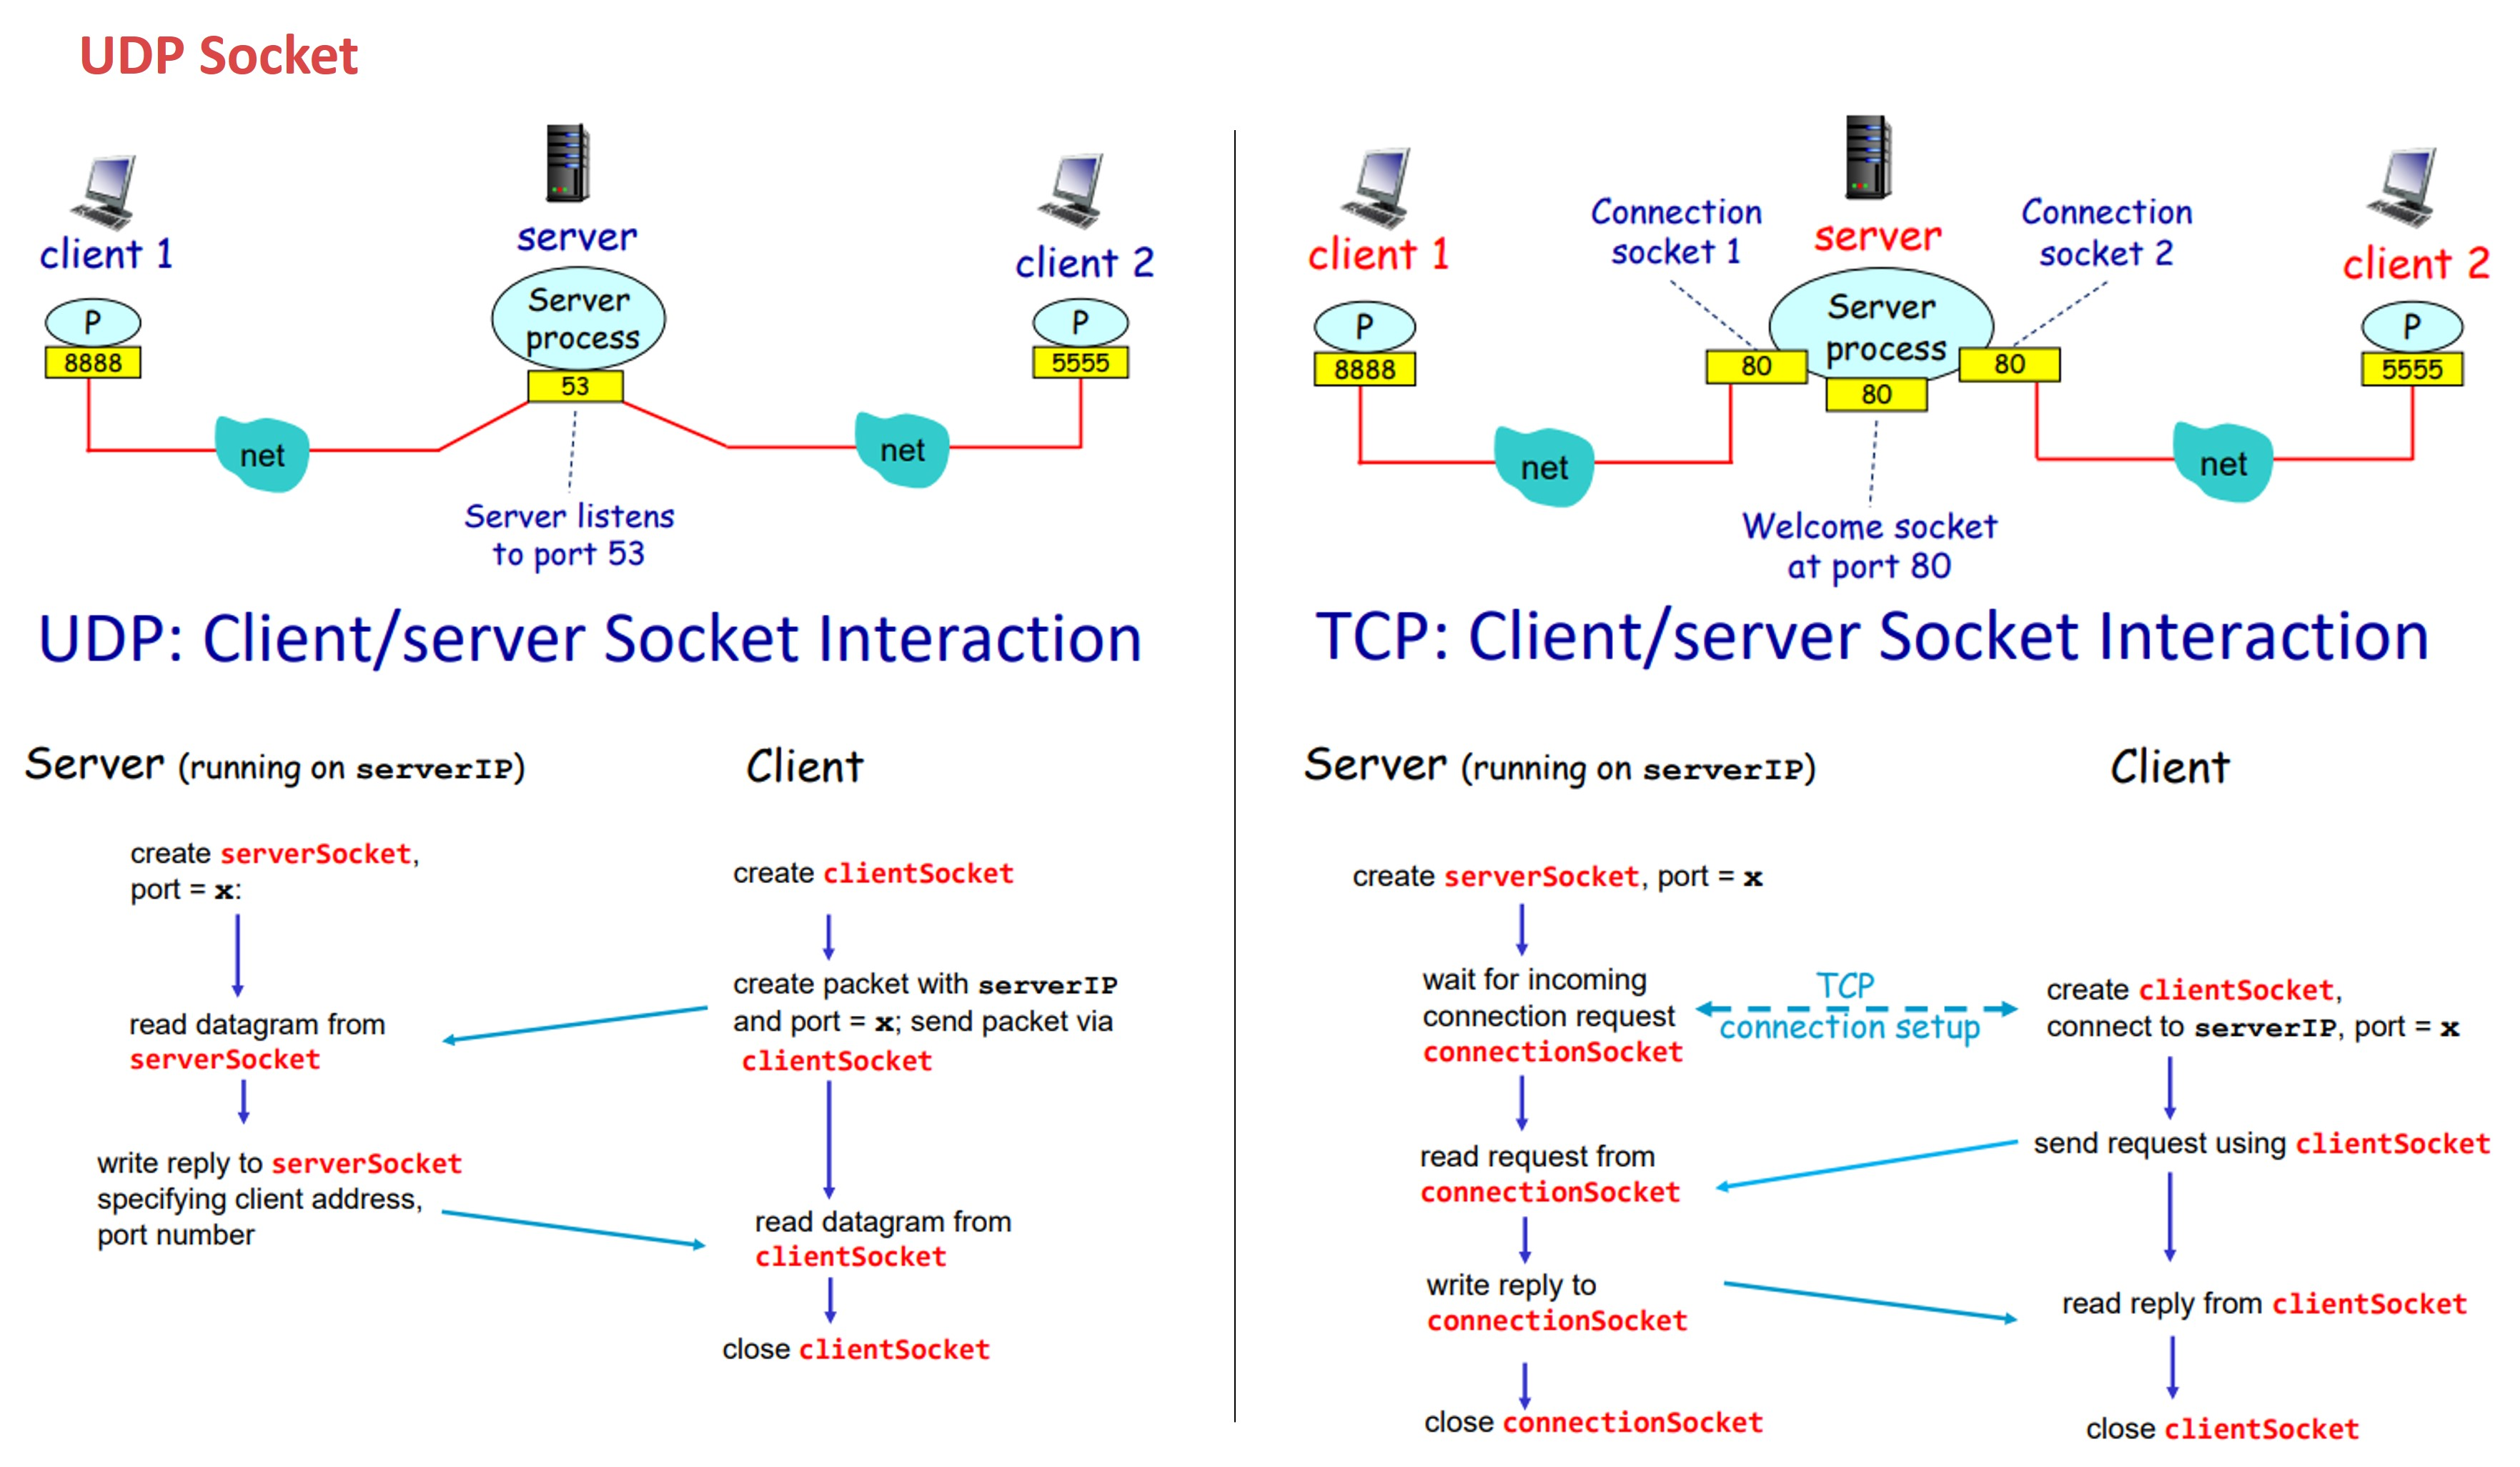
\includegraphics[width=1\linewidth]{socket}}
\begin{itemize}
\item \textbf{TCP vs. UDP Differences}
\item In TCP, two processes communicate as if pipe between them. The pipe remains in place until one of two processes closes it. Sending process doesn’t need to attach a destination IP 
/ port number to the bytes in sending attempt as the logical pipe has been established
\item In UDP, programmers need to form UDP datagram packets explicitly and attach destination IP address / port number to every packet.
\end{itemize}

\vfill \null
\columnbreak

\section{3. Transport}
\subsubsection{Transport Layer Services}
\begin{itemize}
\item Transport layer protocols run in hosts.
\item Sender side: breaks app message into segments (as 
needed), passes them to network layer (aka IP layer).
\item Receiver side: reassembles segments into message, 
passes it to app layer.
\item Packet switches (routers) in between: only check 
destination IP address to decide routing.
running on different hosts
\end{itemize}

\subsubsection{Transport and Network Layer}
\begin{itemize}
\item \textbf{Transport} layer takes care of logical communication
between \textbf{processes}. 
\item \textbf{Network} layer takes care of
logical communication between \textbf{hosts}. (best-effort, unreliable)
\item \textbf{IP Datagram}: Contains source and dest IP addresses, carries one transport layer segment that contains source and dest port numbers.
\end{itemize}



\section{UDP: Connectionless Transport}
\begin{itemize}
\item UDP adds very little service on top of IP.
\item \textbf{Multiplexing at sender}: UDP gathers data, forms packets, passes to IP.
\item \textbf{De-multiplexing at receiver}: UDP receives packets from lower layer, checks dest port, and dispatches them to right processes.
\item \textbf{Unreliable}: UDP transmission used by loss tolerant and rate sensitive apps.
\centerline{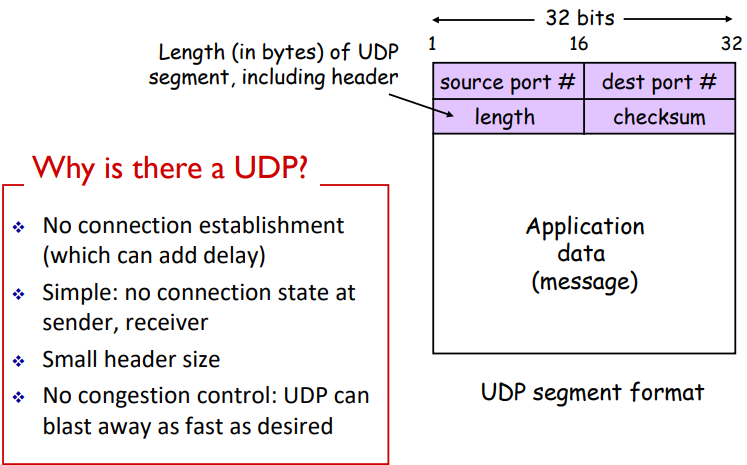
\includegraphics[width=0.8\linewidth]{udpheader}}
\end{itemize}

\subsubsection{UDP Checksum}
\begin{itemize}
\item Allows for error detection, but not correction. May be bit errors when segments are stored and passed in router memory.
\item  Treat UDP segment as a sequence of 16-bit integers.
\item Apply binary addition on every 16-bit integer (checksum field currently 0).
\item If carry from MSB, add 1 to result (wrap).
\item Compute 1’s complement to get UDP checksum.
\end{itemize}

\subsubsection{Principles of Reliable Data Transfer (rdt)}
We need to build a reliable transport layer protocol
on top of unreliable communication.
\begin{itemize}
\item Factors: \textbf{Packet corruption, Packet loss, Packet reordering, Packet (Long) Delay.}
\item Finite State Machines to describe protocol.
\end{itemize}
\medskip
Reliable Data Transfer: \textbf{Service Model}
\centerline{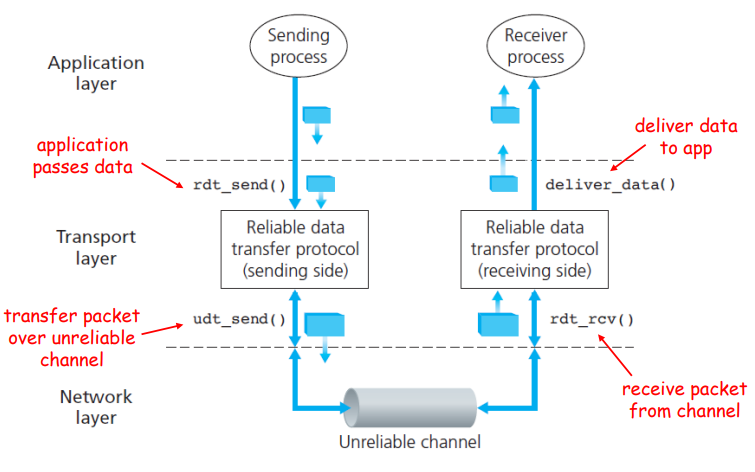
\includegraphics[width=0.8\linewidth]{rdtmodel}}

\subsubsection{rdt 1.0 (Perfectly Reliable)}
\begin{itemize}
\item Assumption: Underlying channel perfectly reliable.
\item Sender creates packet and sends, Receiver extracts and deliver data to application.
\end{itemize}

\subsubsection{rdt 2.0 (Corruptable Data)}
\begin{itemize}
\item Assumption: Underlying channel may flip bits. Use \textbf{stop and wait} (for receiver response) protocol. 
\item Receiver uses checksum to detect bit errors, sends NAK if corrupted. Sender resends if NAK received.
\item \textbf{Problem: If ACK or NACK corrupted}, no guaranteed way to recover. If packet resent, the receiver will not know it’s a duplicate.
\end{itemize}

\subsubsection{rdt 2.1}
\begin{itemize}
\item Add \textbf{sequence number to packet}, alternate 1 \& 0. Sequence number detects duplicates. 
\item Same as rdt2.0, but receiver knows if it is duplicate.
\end{itemize}
\medskip
\centerline{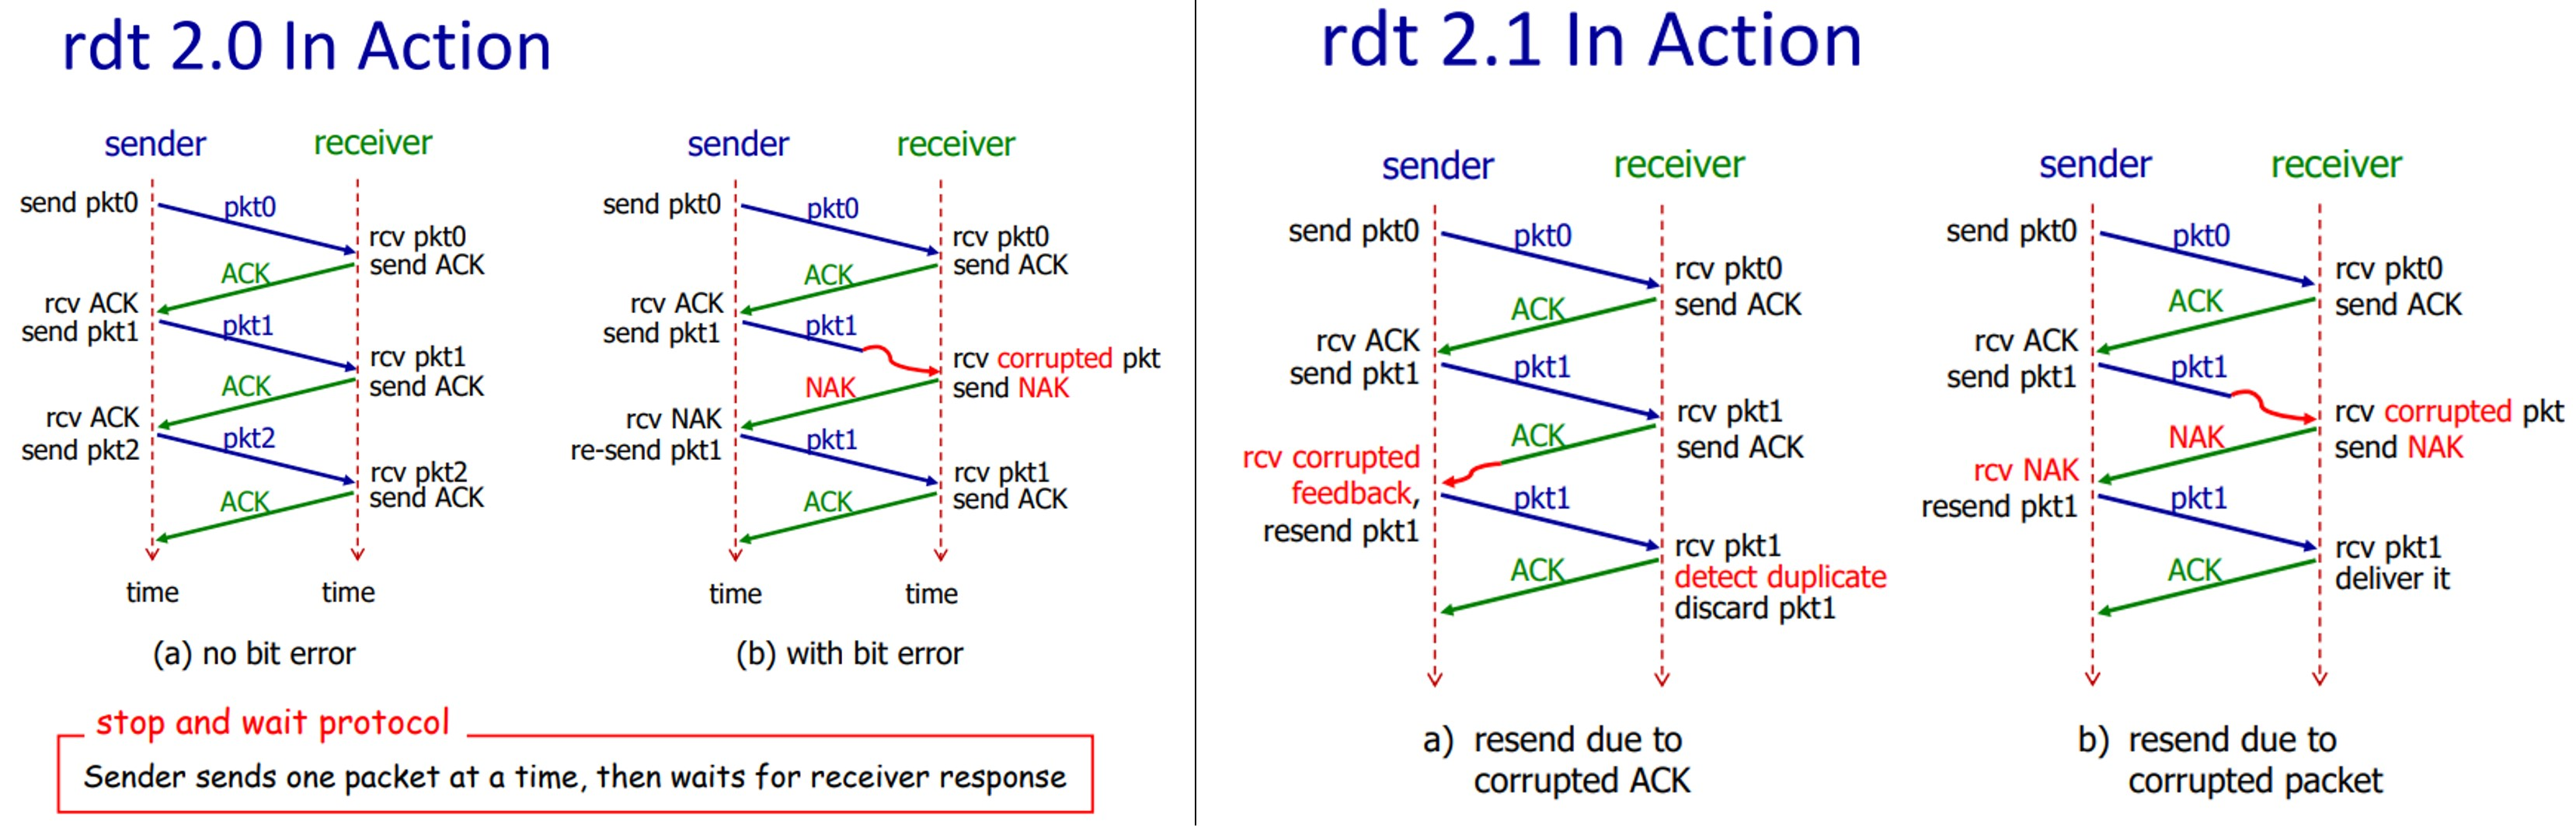
\includegraphics[width=1\linewidth]{rdt2.0-1}}

\subsubsection{rdt 2.2}
\begin{itemize}
\item \textbf{Use ACK of last packet sequence number for NAK.}  
\item Receiver explicitly include seq. no, duplicate ACKs results in retransmit current pkt.
\end{itemize}
\smallskip
\centerline{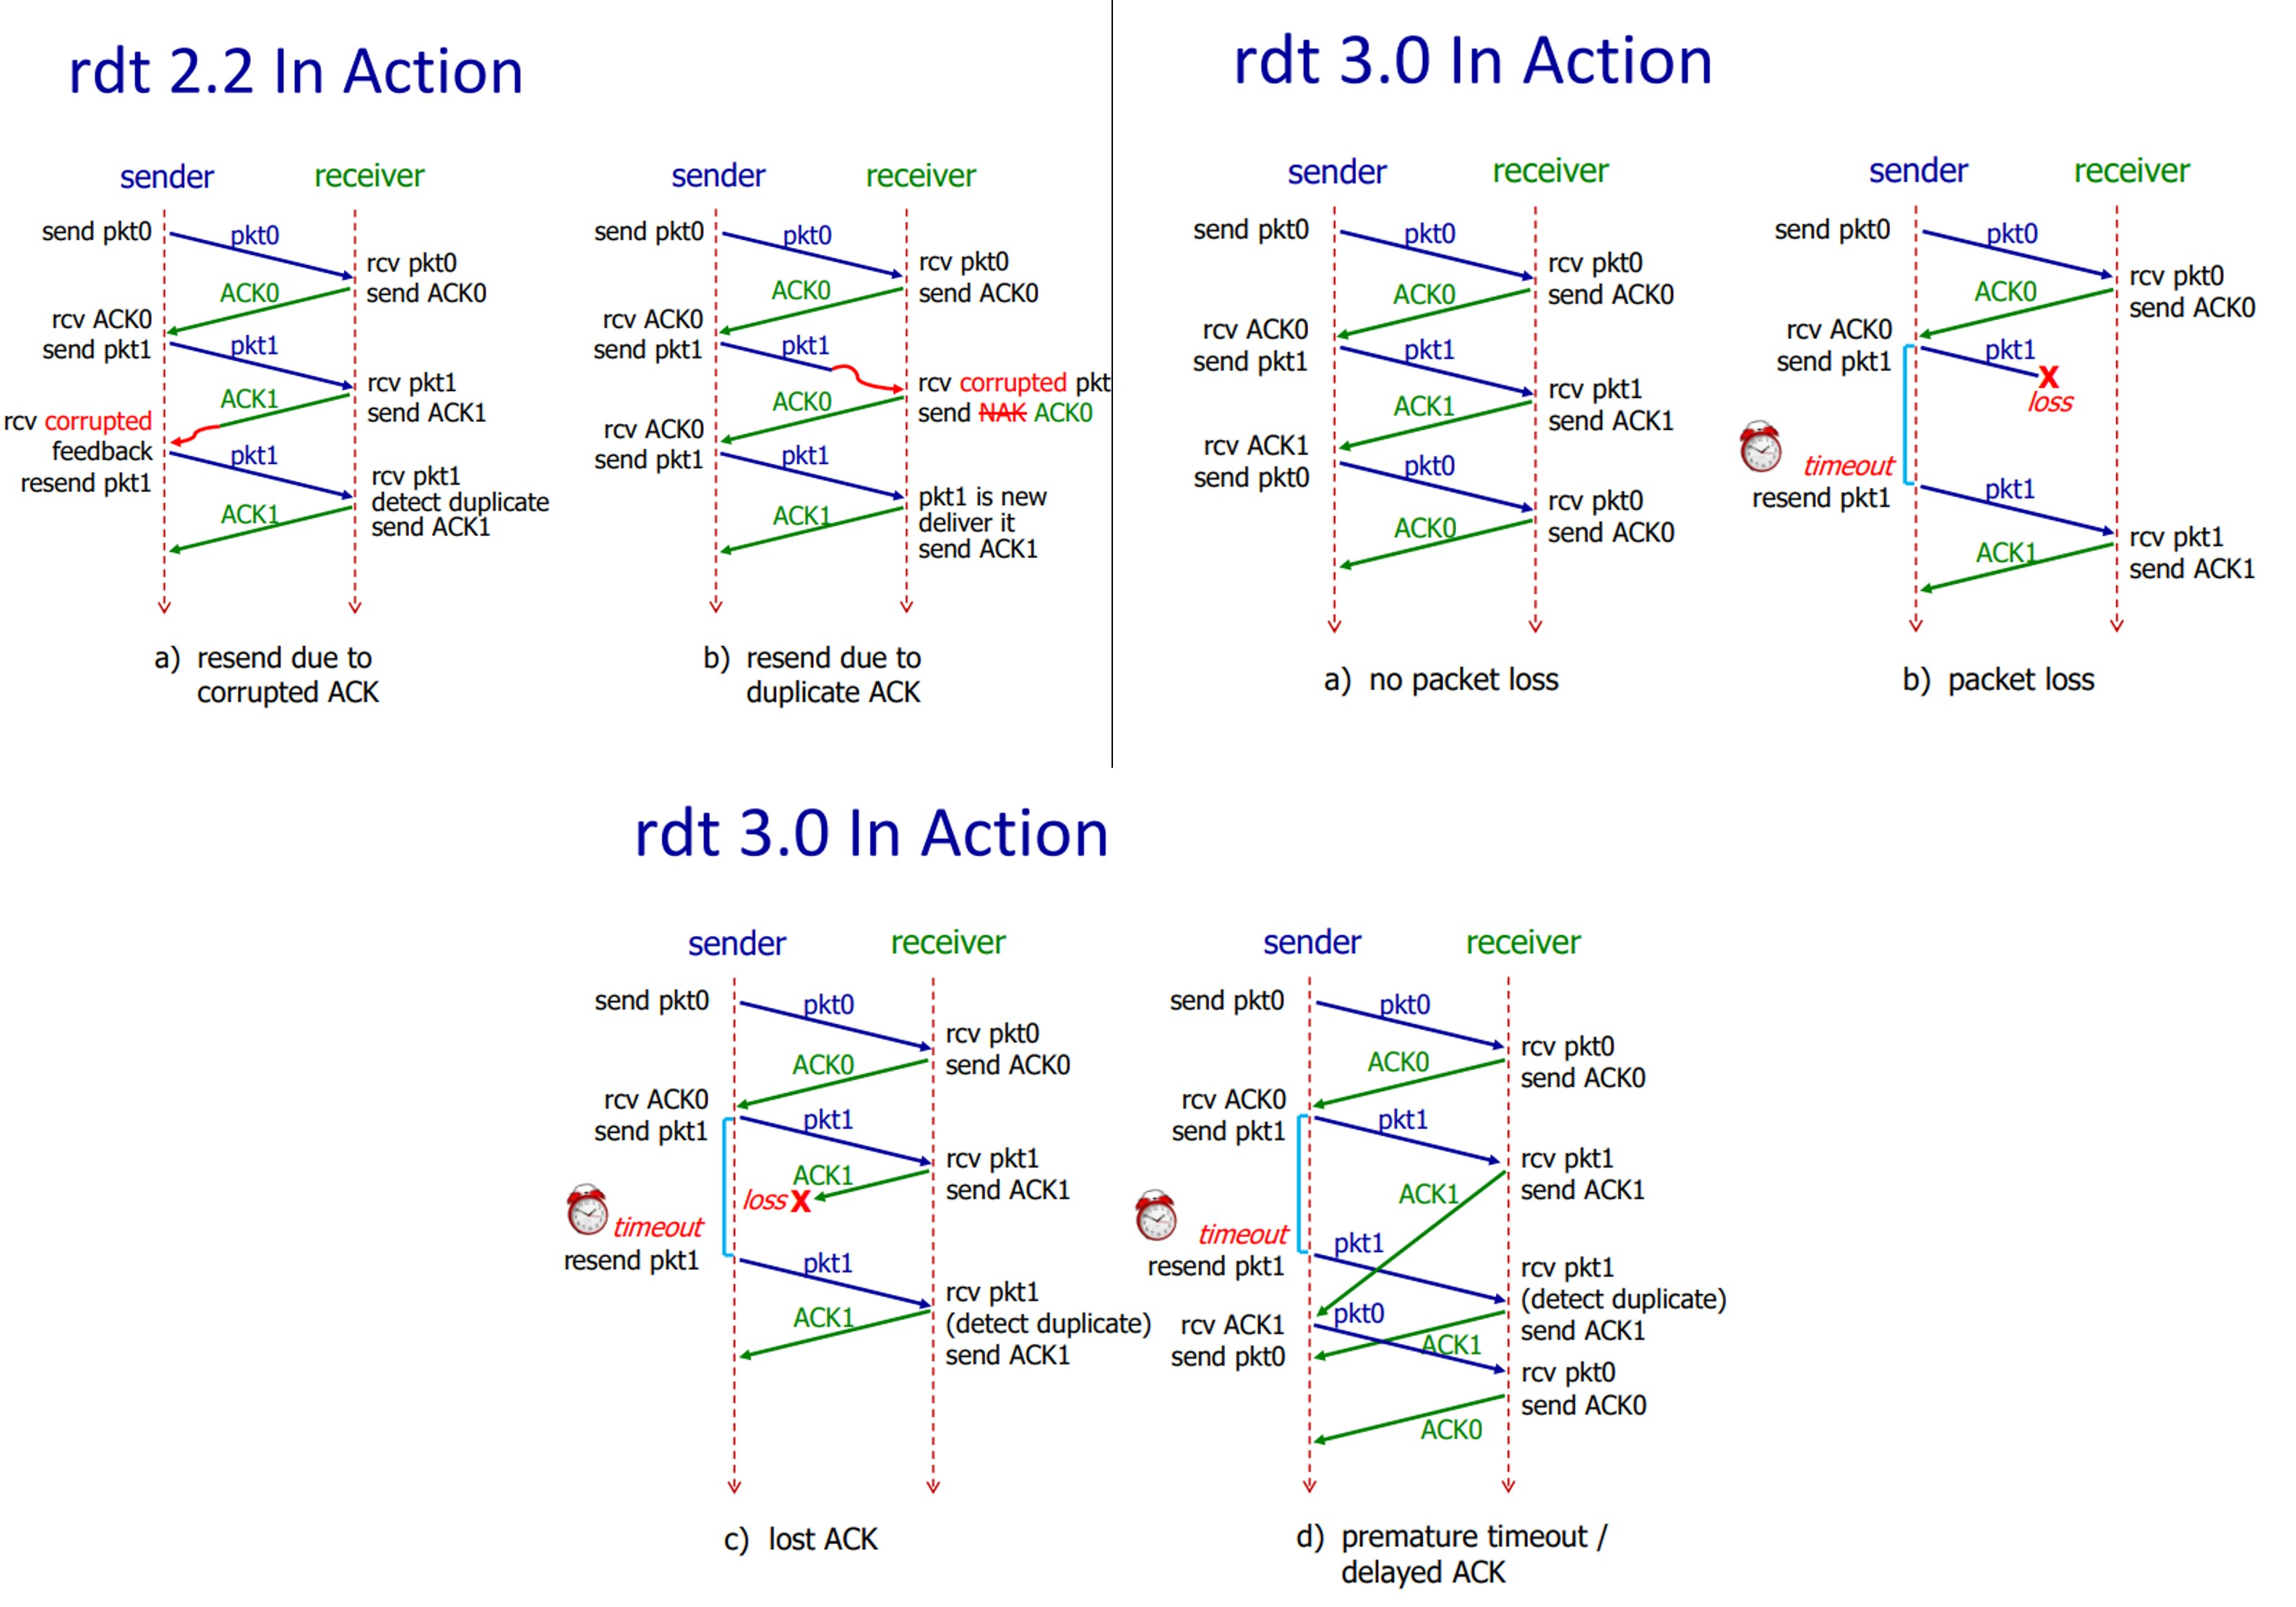
\includegraphics[width=1\linewidth]{rdt2.2-3}}

\subsubsection{rdt 3.0 (Corruptable, Lossy, Delay)}
\begin{itemize}
\item Assume corruption, packet loss/delay, no re-order. 
\item To detect packet loss, use \textbf{sender timeout}. Sender retransmits if no ACK received till timeout.
\item  If packet/ACK just delayed, retransmission may generate duplicates but receiver can use seq. no. to detect.
\item \textbf{rdt 3.0 performance}: Utilisation rate of sender low. For RTT 30ms, $L$ = 8000b, link 1GBps, $d_{trans}$ = 0.008ms, send 8000 bits per 30.008ms. Utilisation 0.027\%.
\item Stop and Wait limits use of physical resources.
\end{itemize}

\subsubsection{Pipelining}
\begin{itemize}
\item  \textbf{Pipelined Protocols}: sender allows multiple, “in-flight”, yet to-be-acknowledged packets. \\
• range of sequence numbers must be increased \\
• buffering at sender and/or receiver
\item Number of packets sent at once is called \textbf{window size}.
\item \textbf{Benchmarked Pipelined Protocols}: Go-Back-N (GBN), Selective Repeat (SR).
\item Assumption of corruption, packet loss / delay.
\end{itemize}

\subsubsection{Go-back-N}
\begin{itemize}
\item Sliding window, slides forward only when ACK received for the leftmost packet in window.
\item Requires $k$ bits in packet header for $2^k$ sequence number.
\item Sender keeps only 1 timer for oldest unACKed packet.
\item Receiver only accepts ACK packets that arrive in order, \underline{discards} out of order packets ACK last in-order sequence number. (cumulative ACK).
\end{itemize}
\smallskip
\centerline{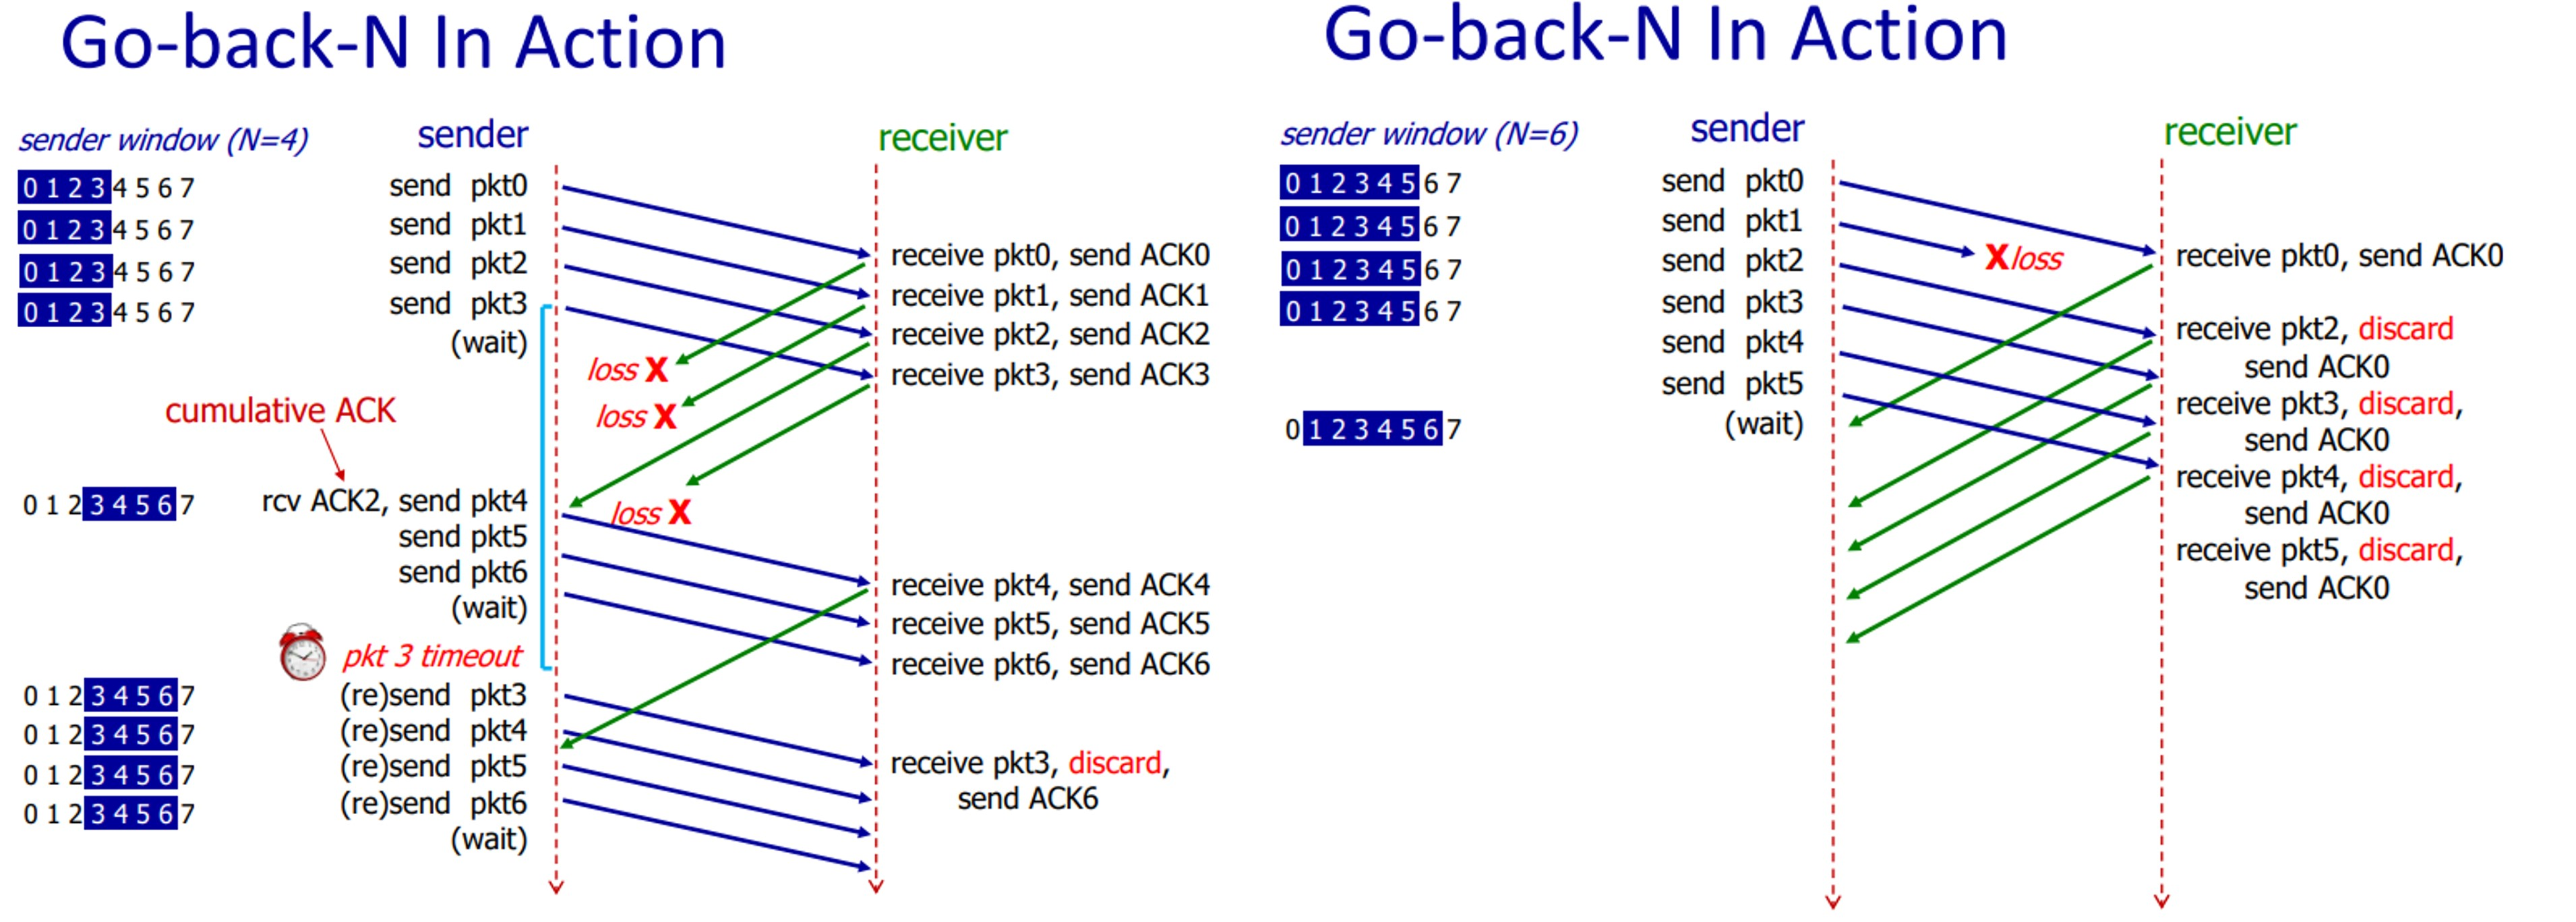
\includegraphics[width=1\linewidth]{gobackn}}

\subsubsection{Selective Repeat}
\begin{itemize}
\item Receiver individually acknowledges all correctly received packets.
\item Buffers out-of-order packets, for eventual in-order delivery to upper layer.
\item Sender maintains timer for each unACKed packet, When timer expires, retransmit only unACKed packet.
\end{itemize}
\smallskip
\centerline{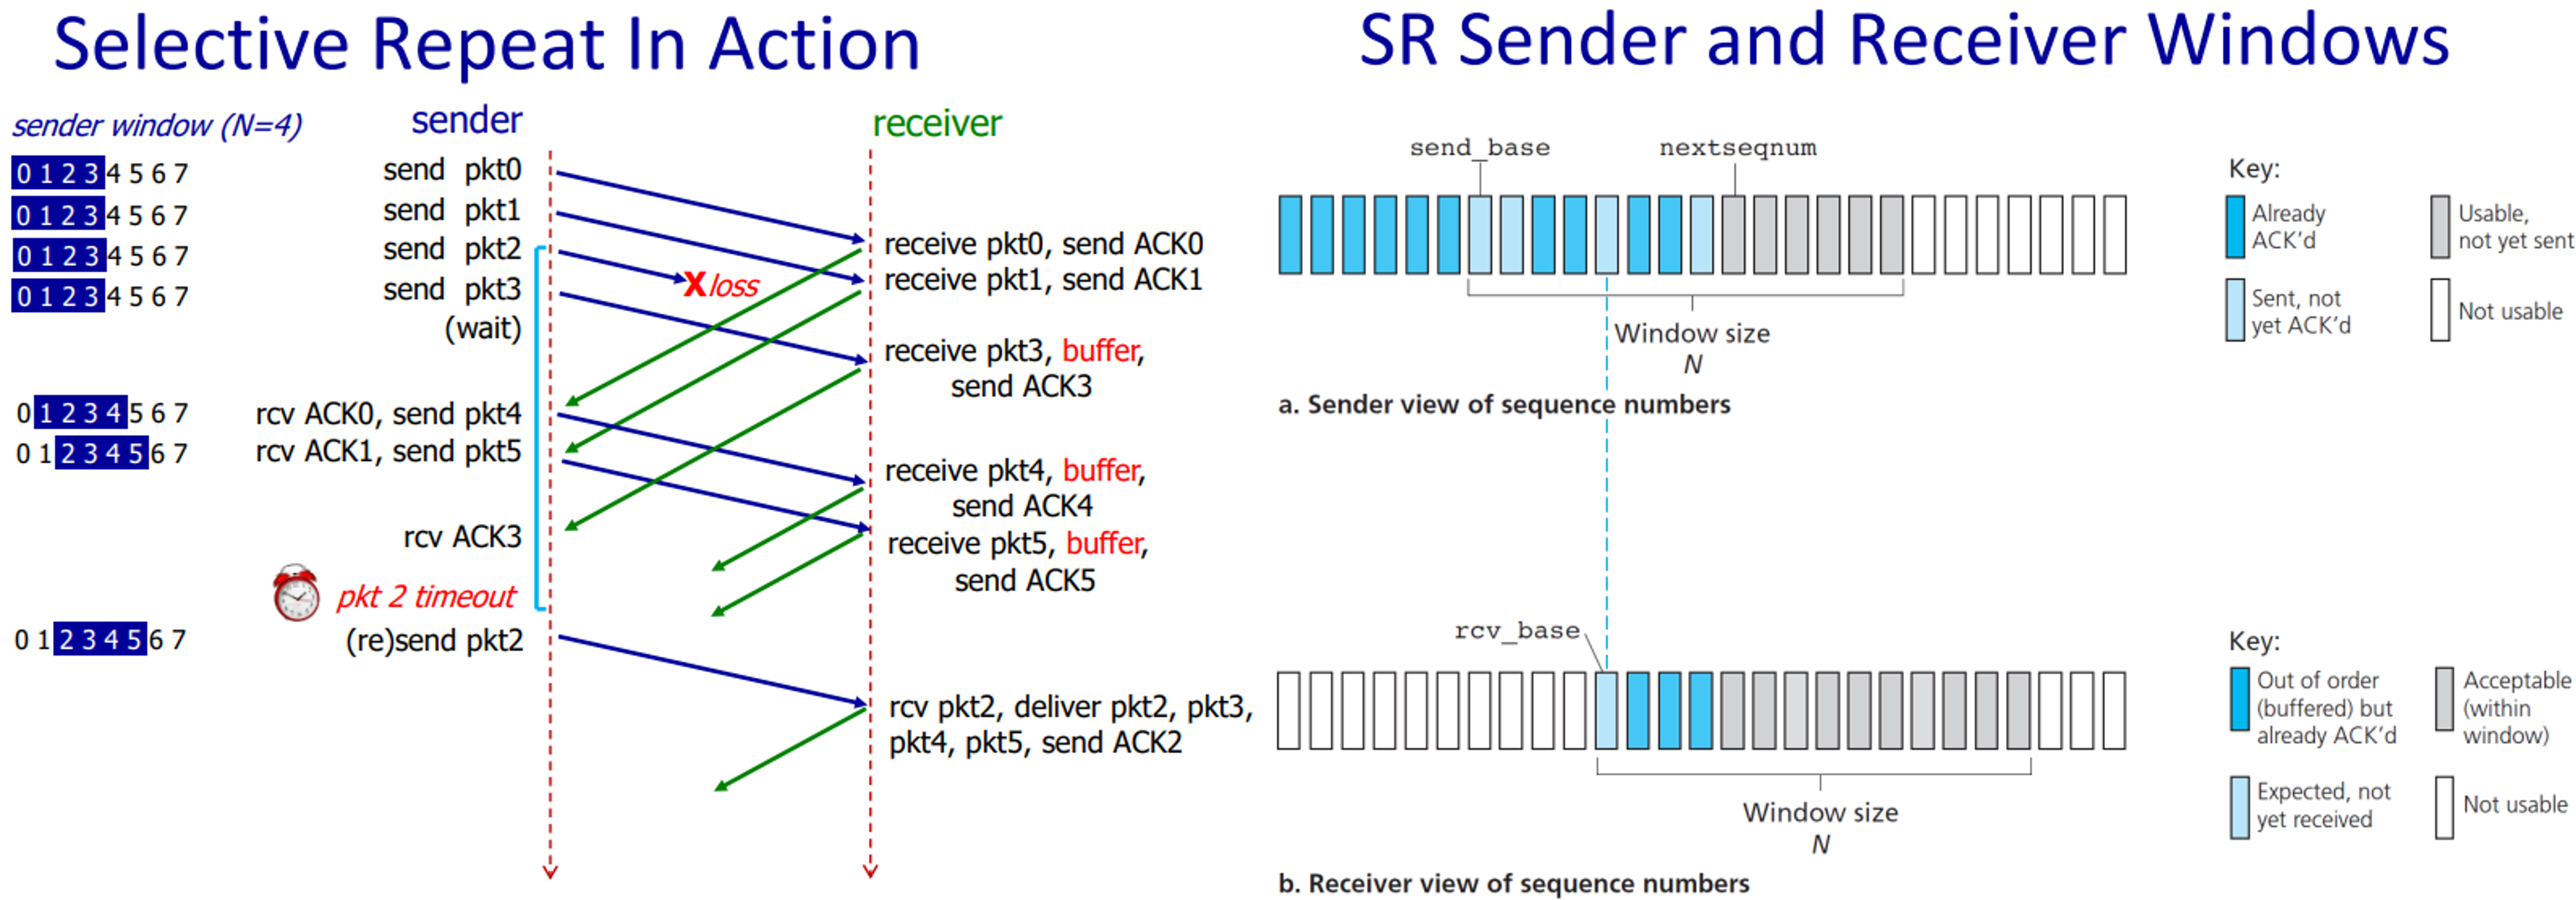
\includegraphics[width=1\linewidth]{selectiver}}



\section{TCP: Connection-oriented Transport}
\begin{itemize}
\item \textbf{Connection oriented}: handshake before sending data. \textbf{Point to point}: one sender, one receiver. The connection is \textbf{duplex} (bidirectional data flow). \textbf{Reliable in-order}.
\item TCP socket is fully identified by four-tuple: (source IP addr, source port no., dest IP addr, dest port no.). 
\item \textbf{Multiplexing}: TCP gathers data from processes, form transport-layer segments including app data and 4-tuple pass to network layer. 
\item \textbf{Demultiplexing}: Connection socket created, server already noted 4-tuple. Subsequent packets directed, or demultiplexed, to the appropriate socket using those 4 values.
\item TCP creates \textbf{buffers} after handshaking. 
\end{itemize}

\subsubsection{TCP Segment / Header}
\begin{itemize}
\item The maximum segment size (MSS) depends on maximum transmission unit (MTU). 
\item Generally MSS is 1460 bytes, (MTU is 1500 bytes for Ethernet and PPP link-layer protocols.) 40 bytes split half for TCP and IP header.
\item TCP Seq. no is "byte no.", first b of data in segment.
\item TCP Ack. no is "seq no." of next b expected by receiver.
\item Checksum computation uses 1s complement (UDP same)
\smallskip
\centerline{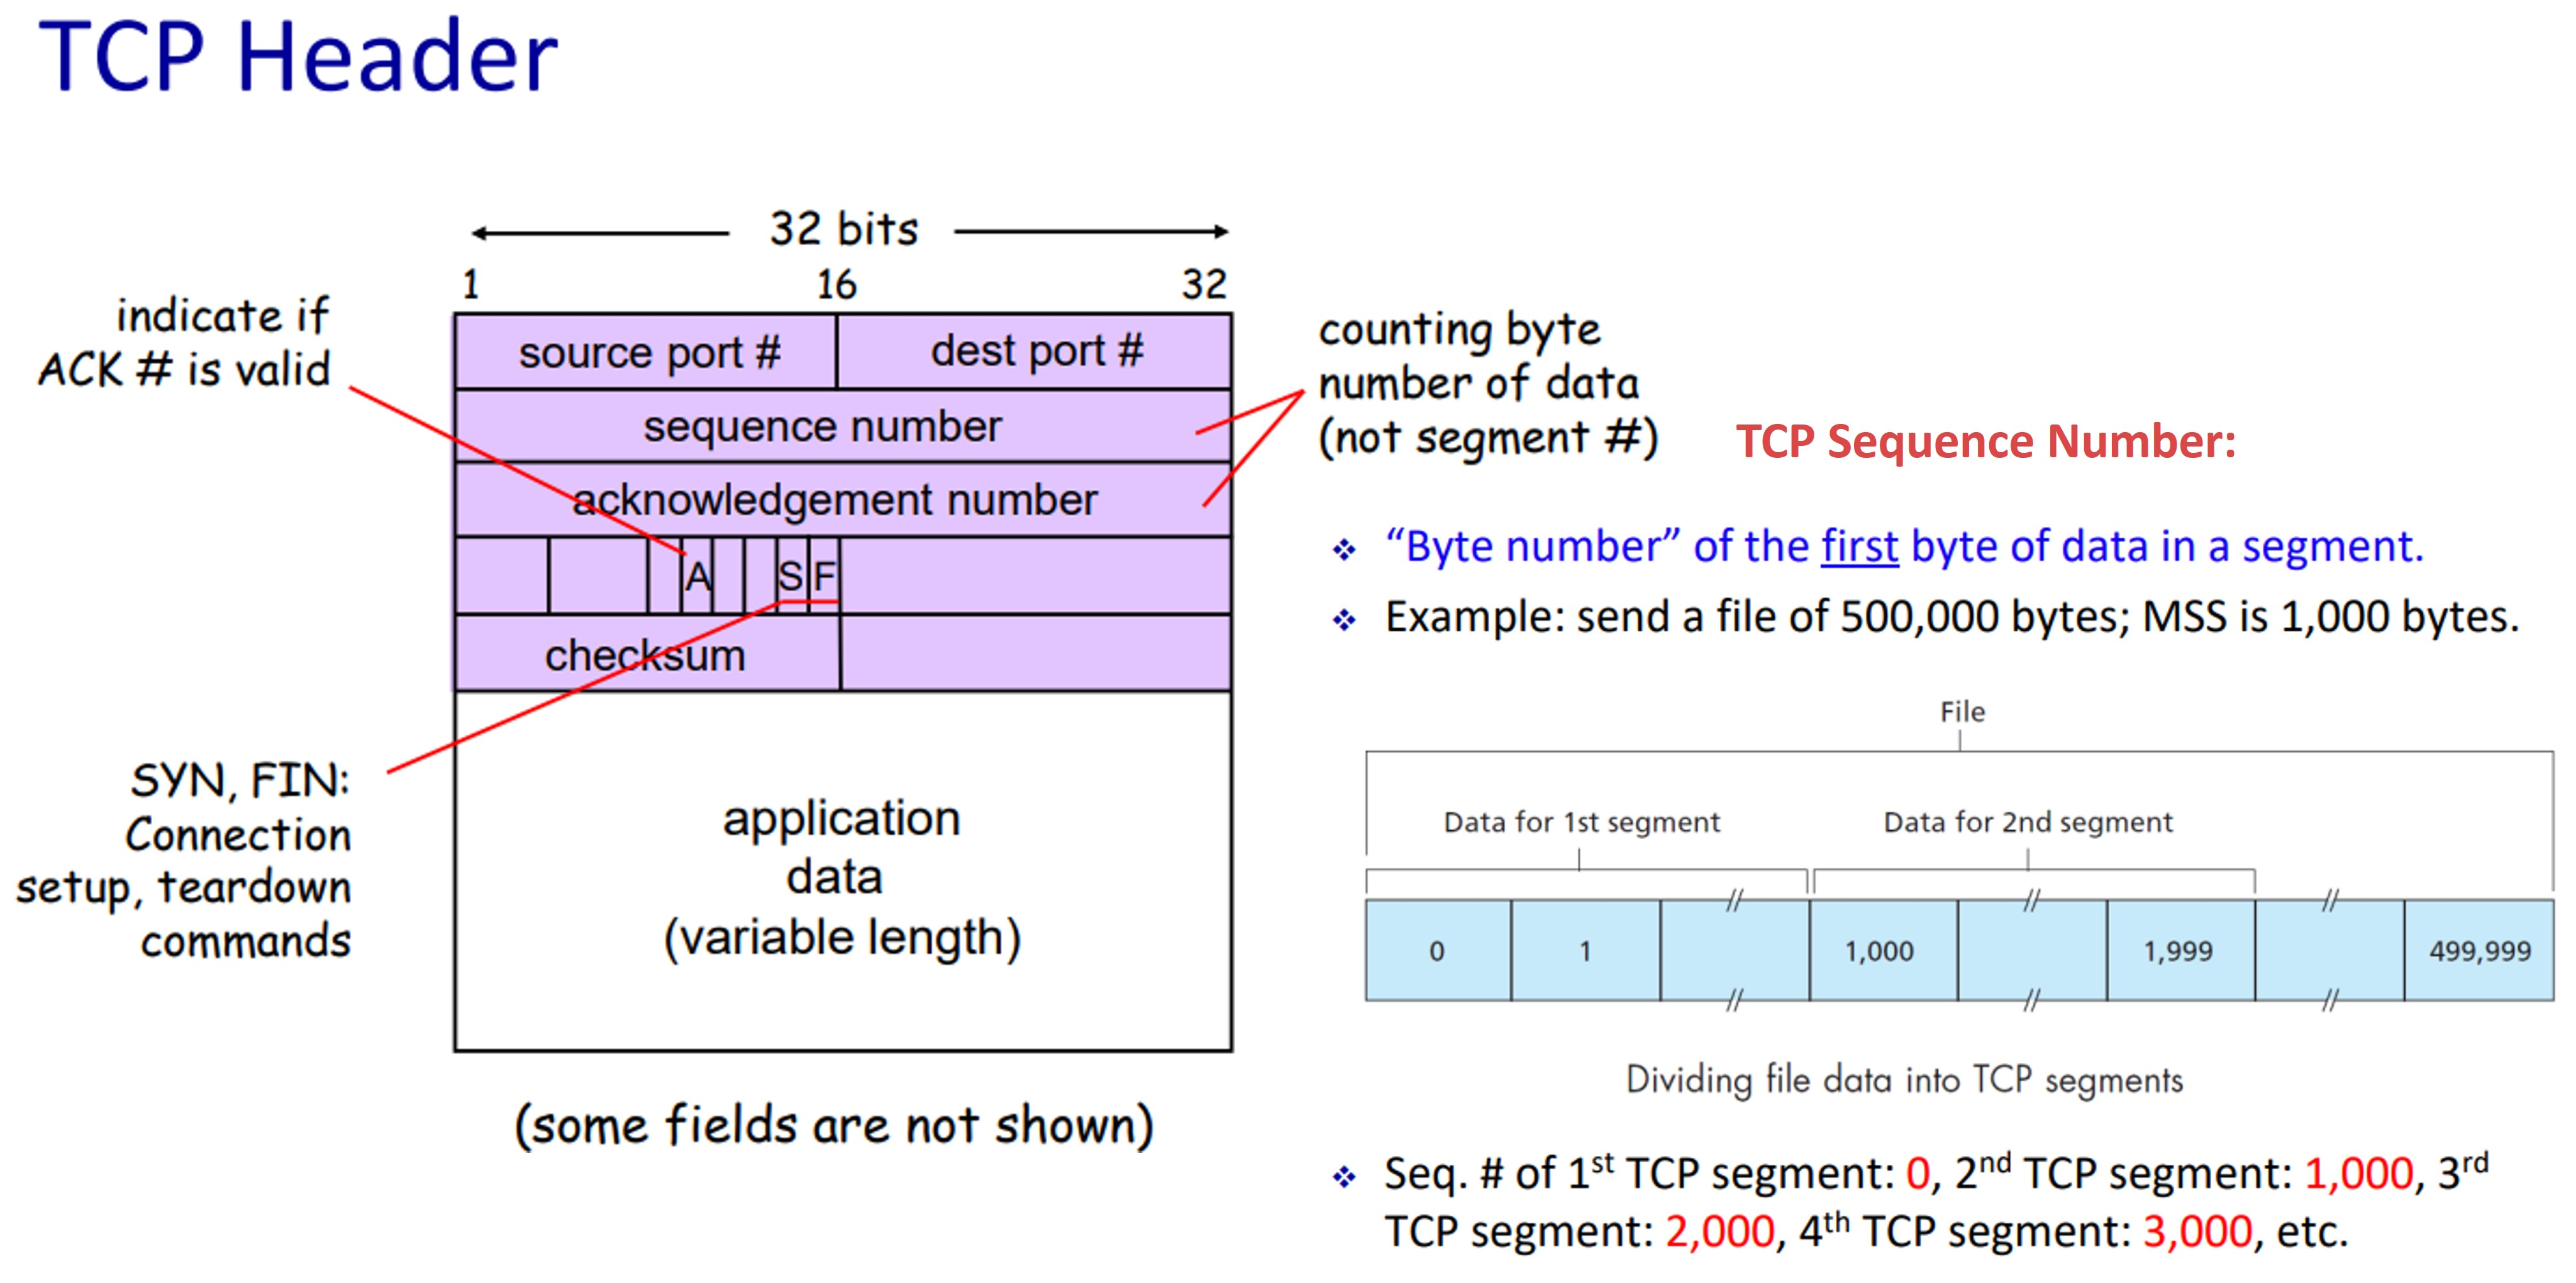
\includegraphics[width=1\linewidth]{tcpheader}}
\medskip
\centerline{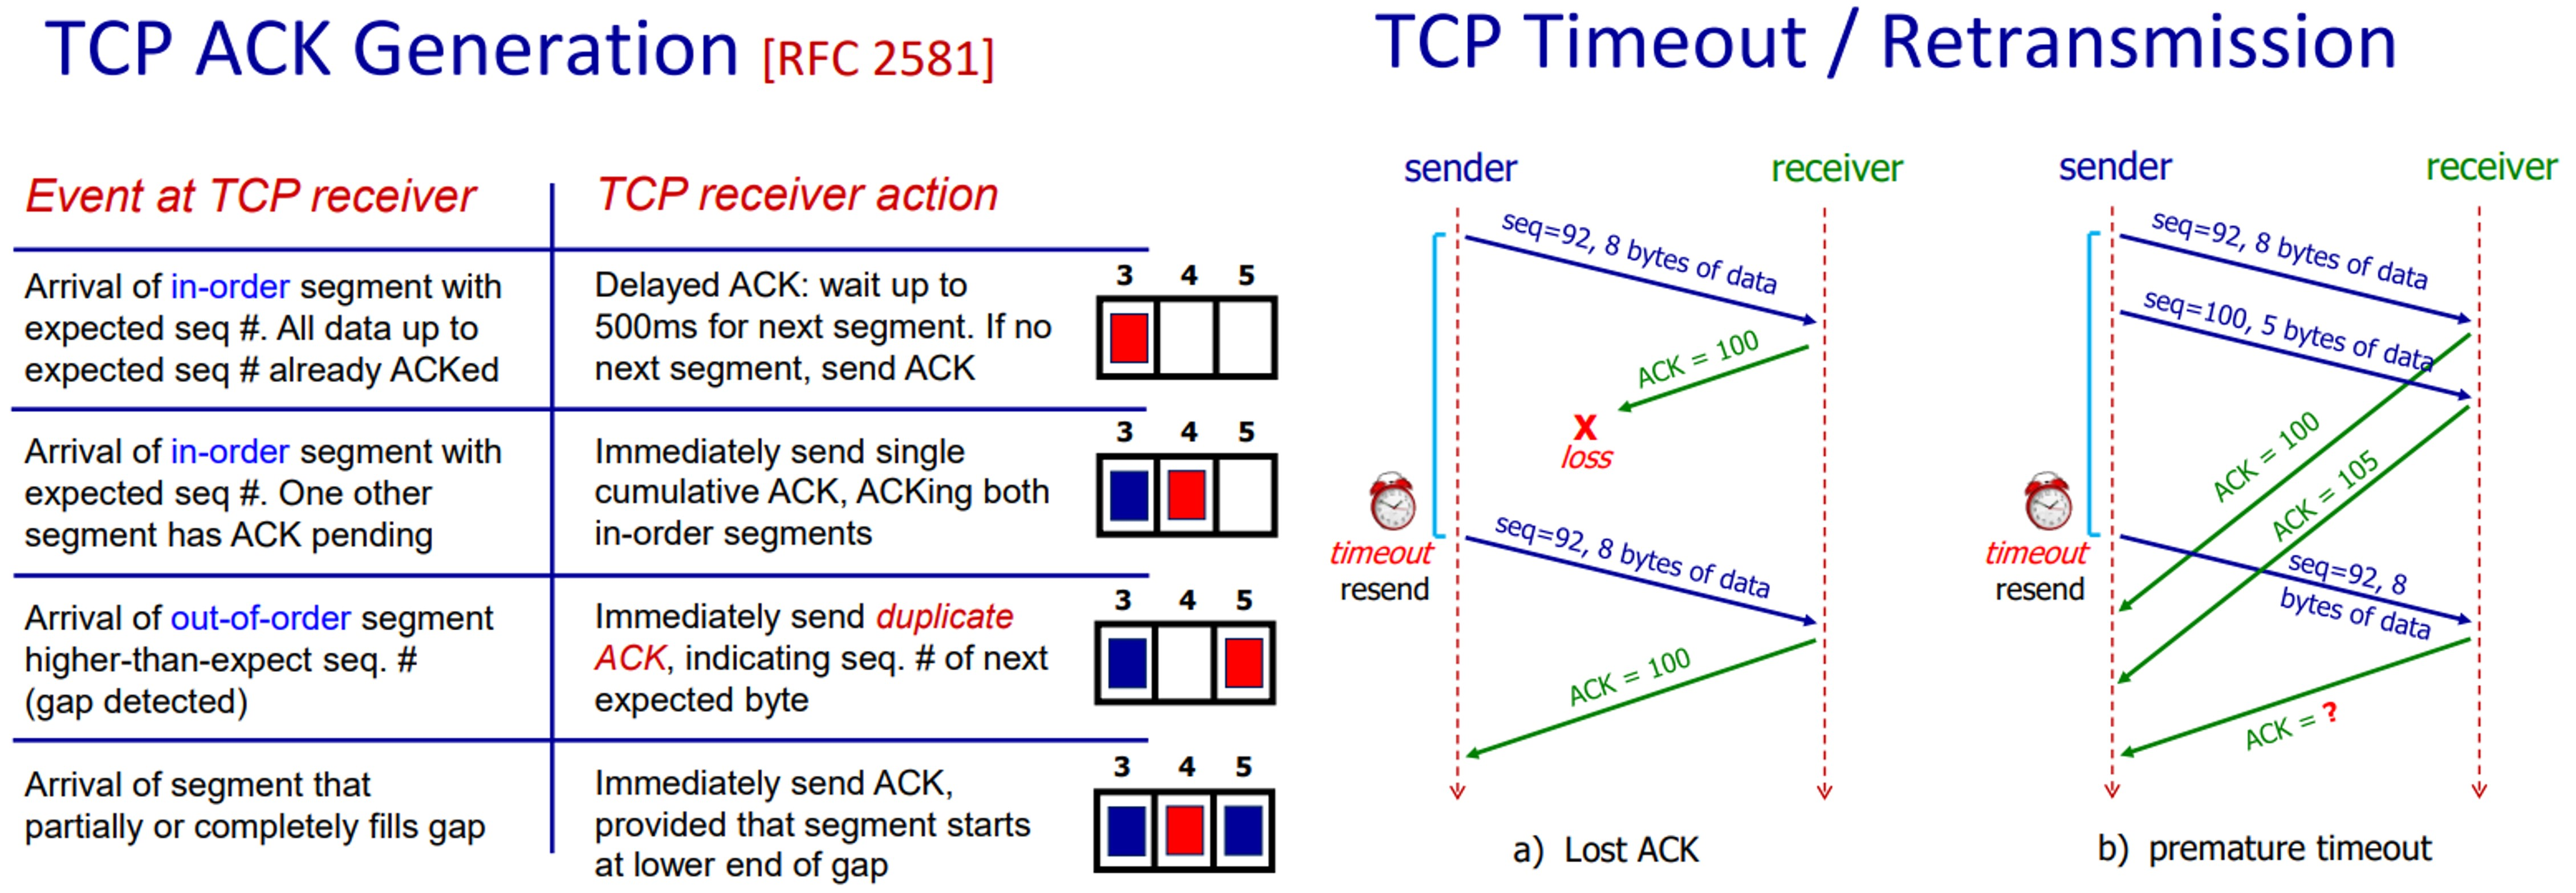
\includegraphics[width=1\linewidth]{TCPACKgen}}
\item Random initial sequence number: Minimise probability of some segment from previous connection mistaken as from current connection
\end{itemize}

% \vfill \null
% \columnbreak

\subsubsection{TCP Timeout Value}
\begin{itemize}
\item Determining TCP appropriate timeout value:
\item too short timeout: premature timeout and unnecessary retransmissions.
\item too long timeout: slow reaction to segment loss. Timeout interval must be longer than RTT – but RTT varies!
\item TCP computes (and keeps updating) timeout interval based on estimated RTT. (TimeoutInterval = EstimatedRTT + 4*DevRTT)
\end{itemize}

\subsubsection{TCP Fast Retransmission}
\begin{itemize}
\item Timeout period is often relatively long. long delay before resending lost packet.
\item \textbf{Fast retransmission}: If sender receives 4 ACKs for same segment, suppose segment is lost, resend segment (even before timer expires).
\end{itemize}
\smallskip
\centerline{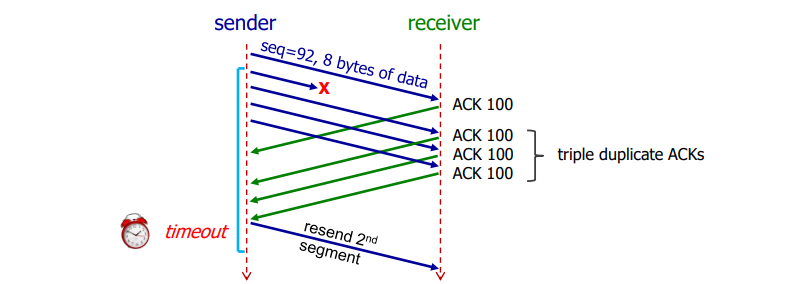
\includegraphics[width=1\linewidth]{fastretransmit}}
\smallskip

\subsubsection{TCP Handshake / Closing}
\begin{itemize}
\item Before exchanging app data, TCP sender and receiver “shake hands”, agree on connection and exchange connection parameters.
\item Closing: Client, server each close their side of connection, send TCP segment with FIN bit = 1 
\end{itemize}
\smallskip
\centerline{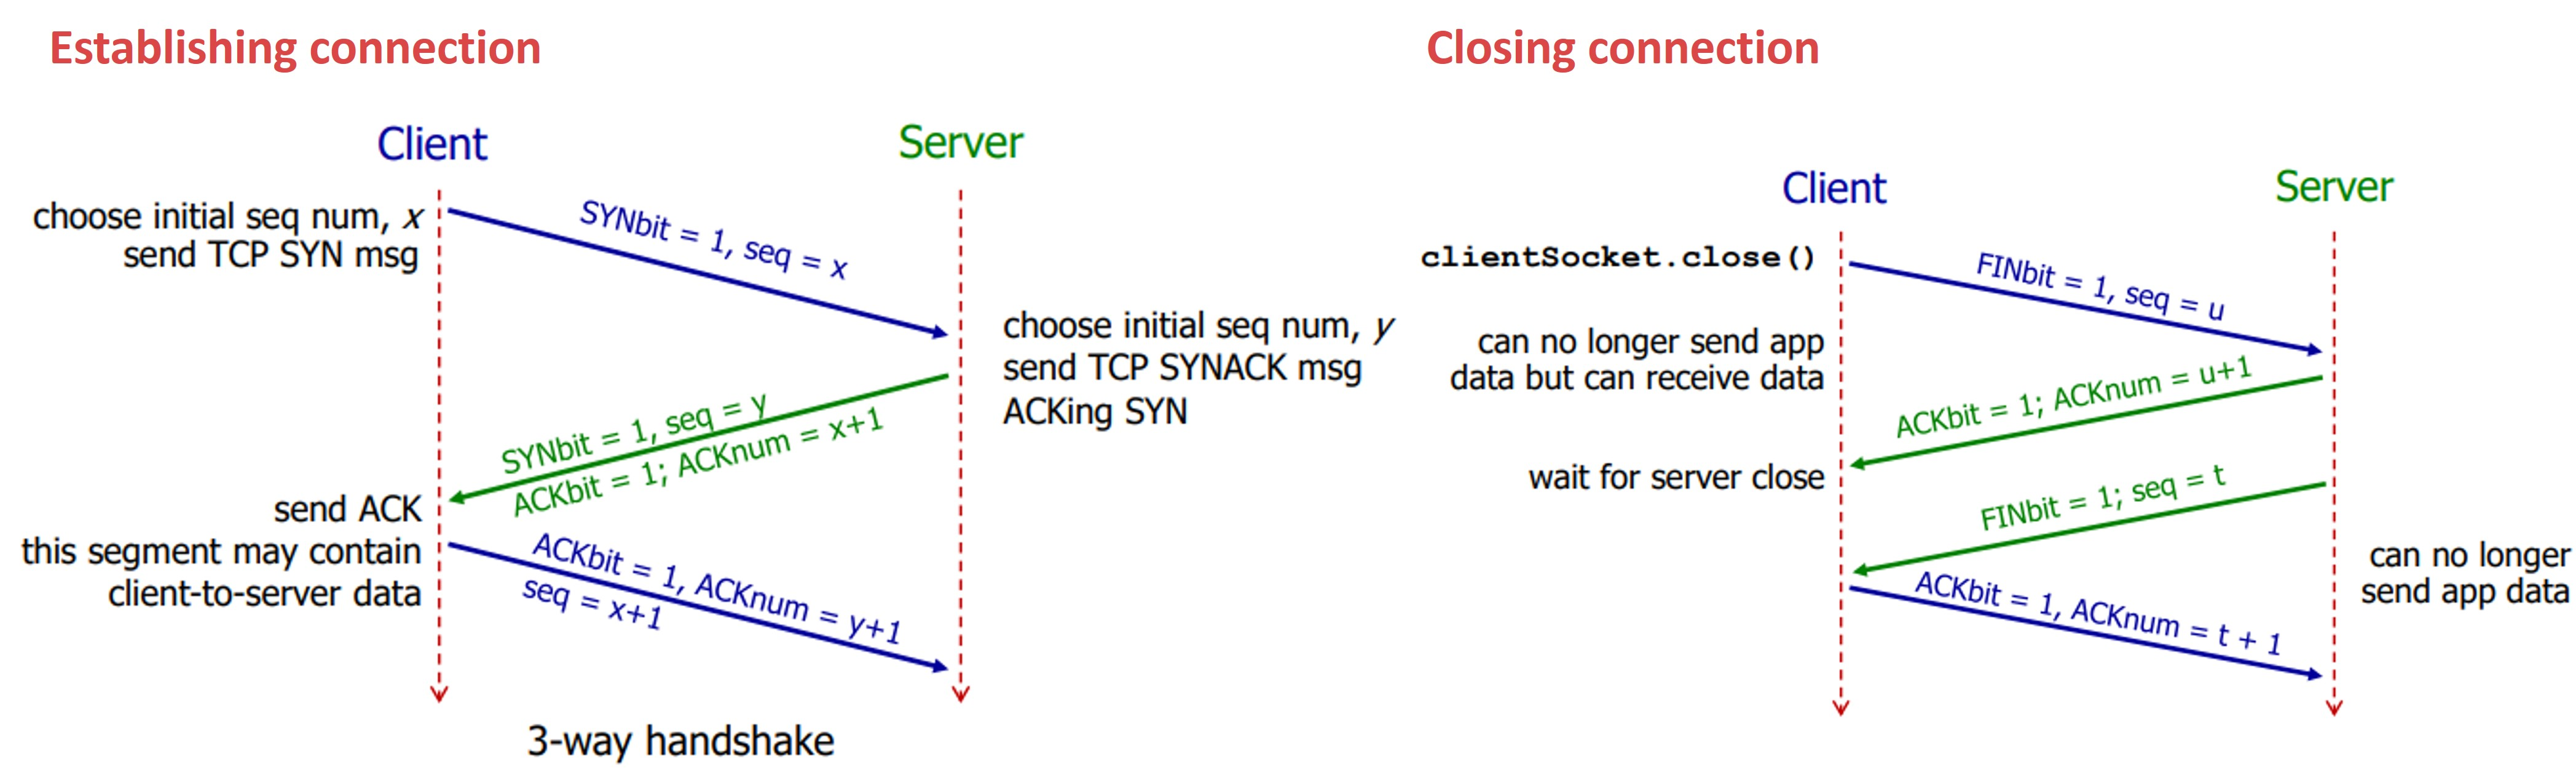
\includegraphics[width=1\linewidth]{tcpconnection}}

% \vfill \null
% \columnbreak

\section{4. Network}
\subsubsection{Network Layer Services}
\begin{itemize}
\item Network layer delivers packets to receiving hosts.
\item Routers examine header fields of IP datagrams passing it.
\item \textbf{Forwarding}: Moving of incoming packet to appropriate output link.
\item \textbf{Routing}: Calculation of path taken by packets from sender to receiver.


\end{itemize}

\subsubsection{IP Address}
\begin{itemize}
\item \textbf{IP address} used to identify host / (router), 32-bit integer expressed in binary/decimal.
\item Host gets an IP address either through manual configuration by sys admin, or auto assigned by a \textbf{DHCP} server.
\end{itemize}

\centerline{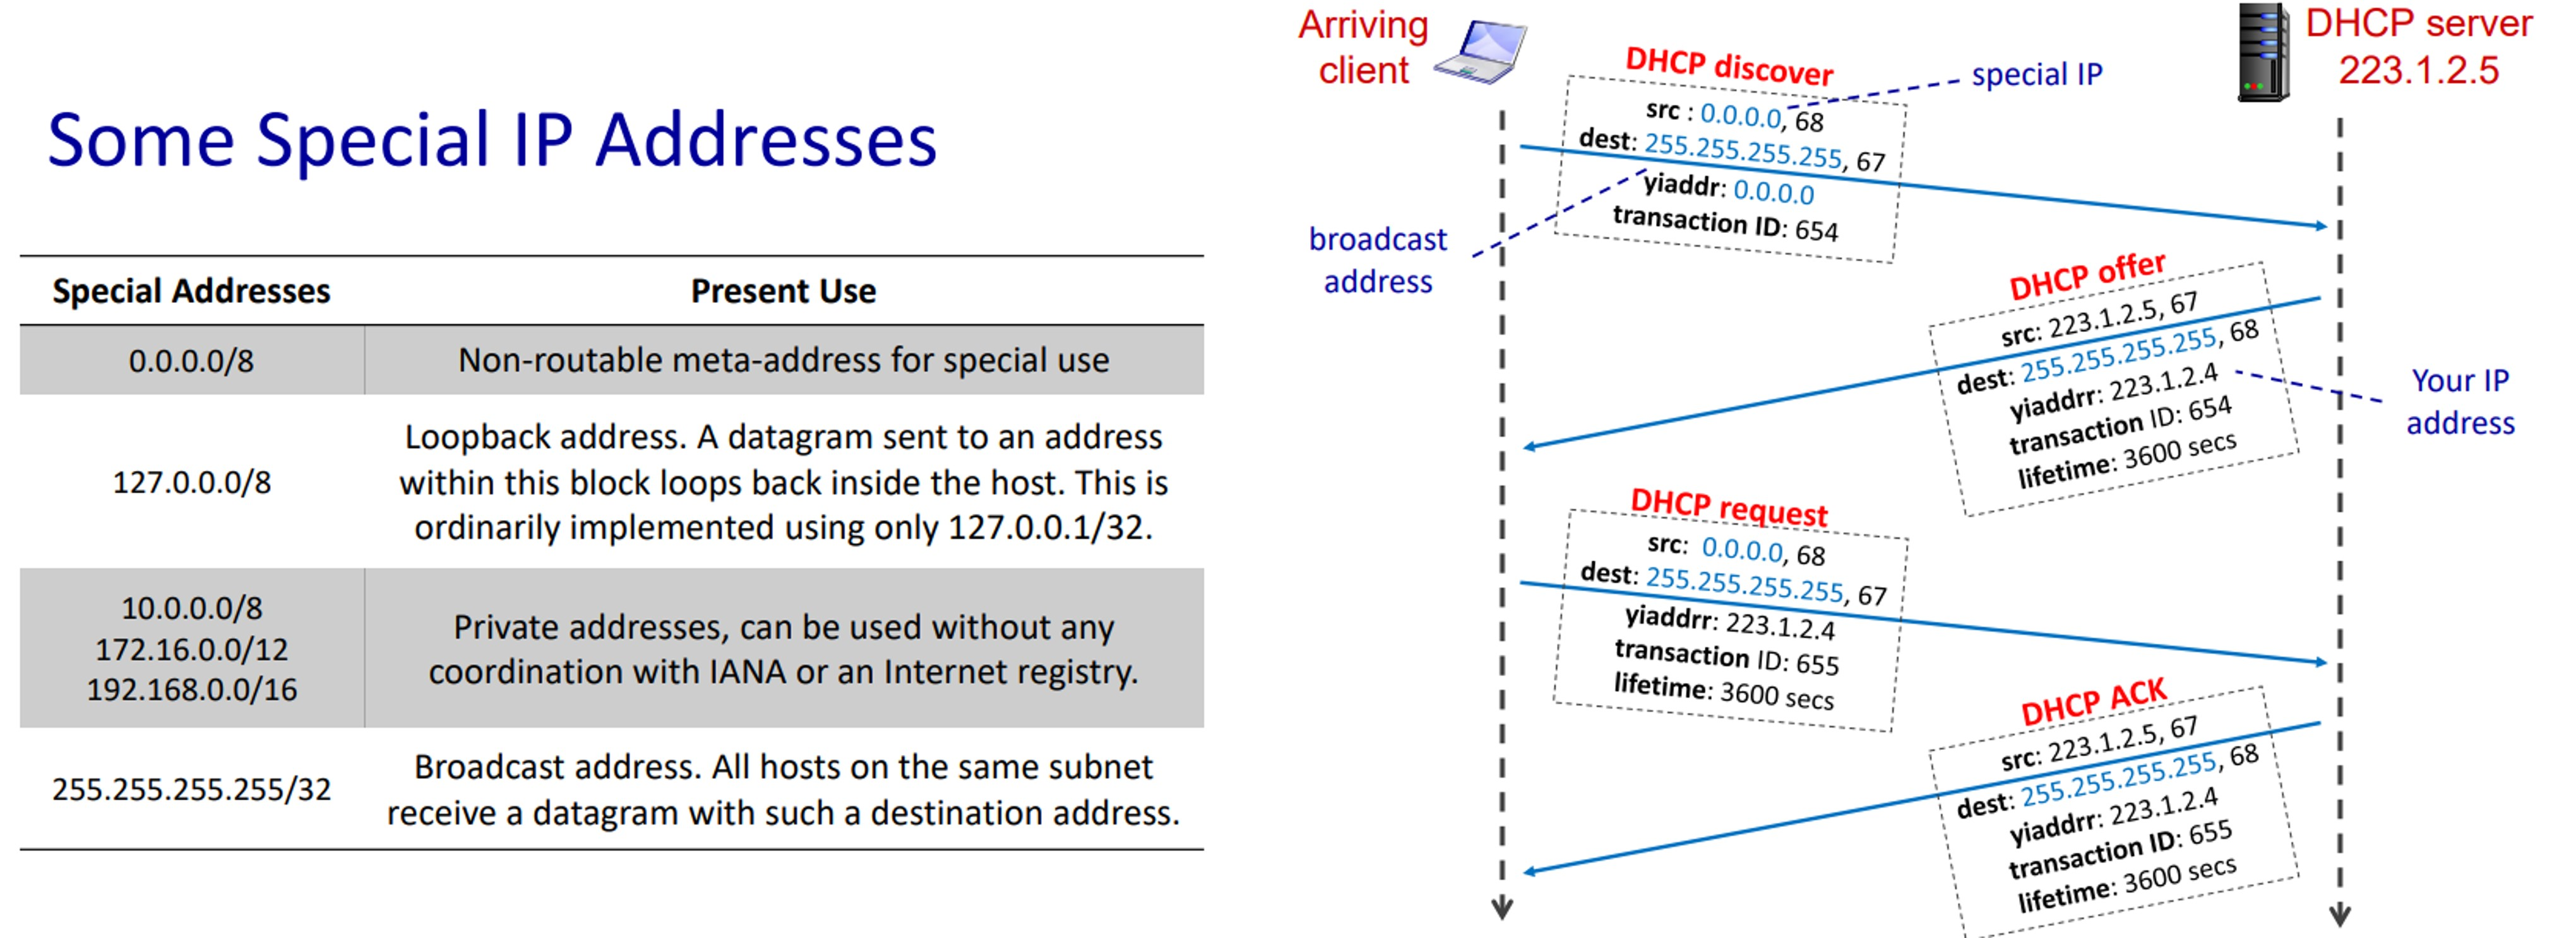
\includegraphics[width=1\linewidth]{dhcp}}

\subsubsection{DHCP: Dynamic Host Configuration Protocol}
\begin{itemize}
\item \textbf{DHCP} allows a host to dynamically obtain its IP address from DHCP server when it joins network.
\item IP address is \underline{renewable}, allow \underline{reuse} of addresses (only hold address while connected), support mobile users to join network.
\item DHCP: 4-step process: Host broadcasts “DHCP discover” message, server responds with “DHCP offer” message, Host requests IP address: “DHCP request” message, DHCP server sends address: “DHCP ACK” message
\item  DHCP may provide host additional network information, e.g. IP of first-hop router, local DNS server, network mask.
\item DHCP runs over \textbf{UDP}. DHCP server port 67, client port 68.
\end{itemize}

\subsubsection{IP Address \& Network Interface}
\begin{itemize}
\item IP address is associated with a network interface.
\item Host usually has one or two network interfaces (e.g. wired Ethernet and WiFi), A router typically has  multiple interfaces.
\item \textbf{IP Addr} comprises network/subnet prefix and host ID.
\end{itemize}

\subsubsection{Subnet}
\begin{itemize}
\item \textbf{Subnet} is a network formed by a group of “directly” interconnected hosts.
\item Hosts in same subnet have same network prefix of IP addr, can physically reach each other without intervening router. They connect to the outside world through a router
\item \textbf{Classless Inter-domain Routing} (CIDR): Internet’s IP address assignment strategy.
\item Subnet prefix of IP addr of arbitrary length, Address format: $a.b.c.d/x$, where $x$ is the no. of bits in subnet prefix of IP addr.
\item \textbf{Subnet mask} is used to determine which subnet an IP address belongs to.
\item made by setting all subnet prefix bits to "1"s and host ID bits to "0"s.
\end{itemize}

\medskip
\centerline{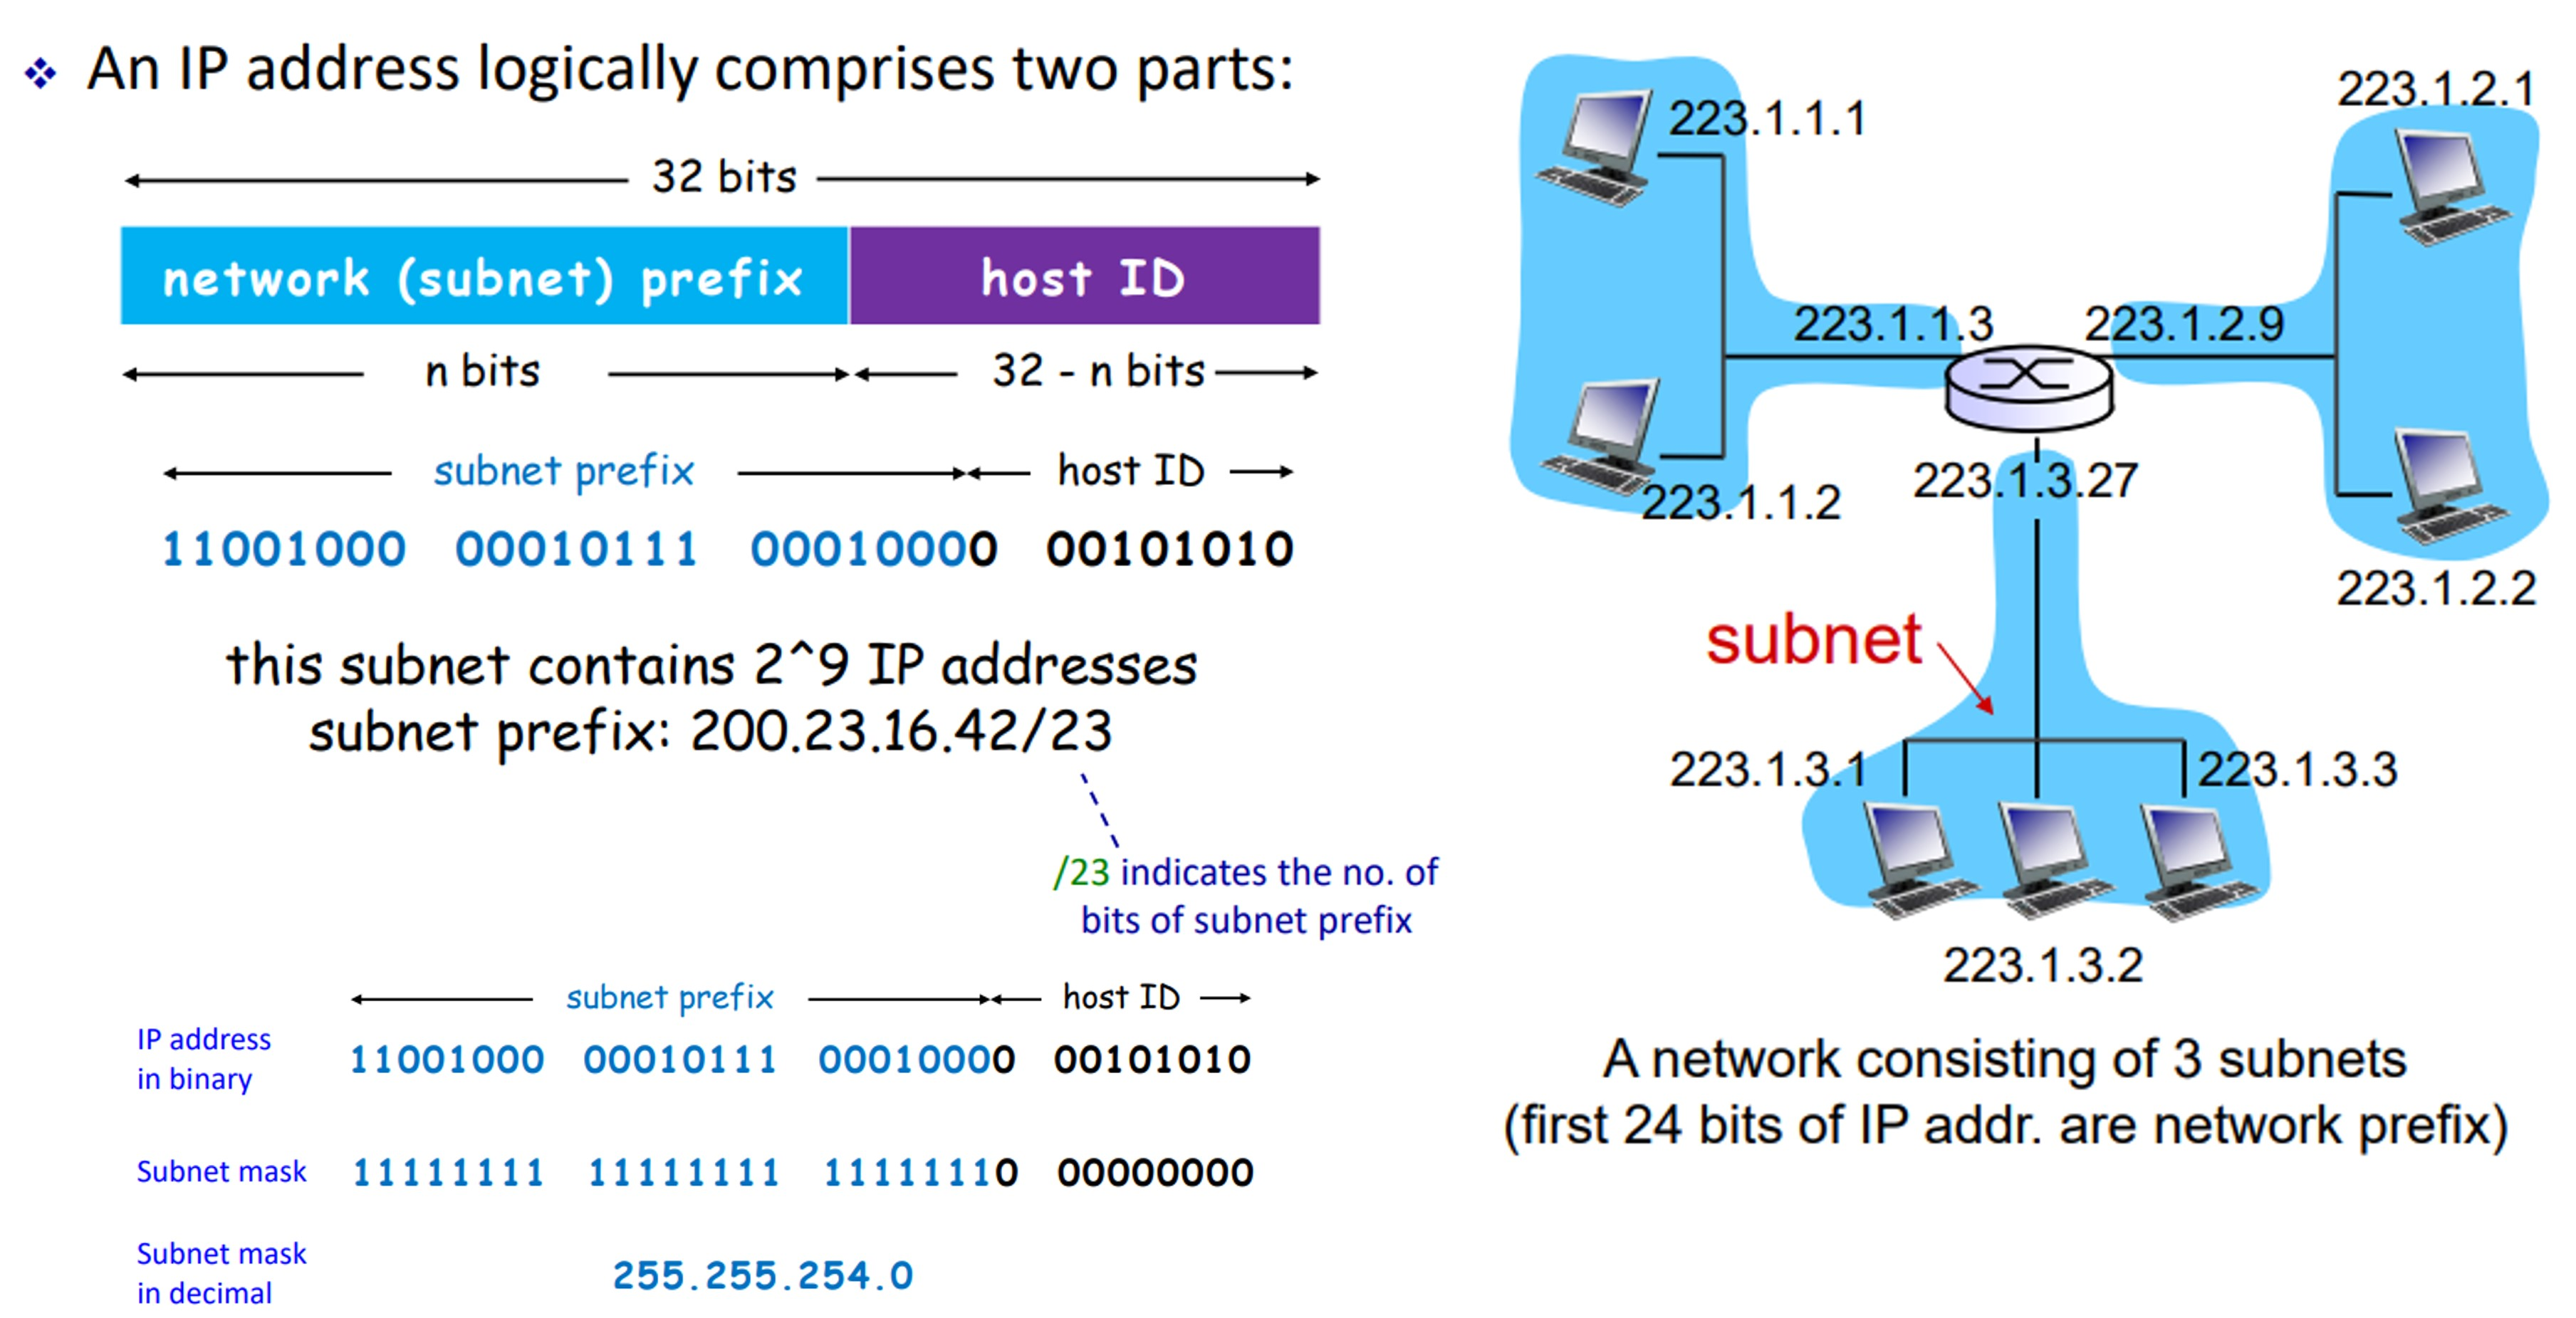
\includegraphics[width=1\linewidth]{ipsubnet}}

\vfill \null

\subsubsection{IP Address Allocation}
\begin{itemize}
\item Organization can buy from registry / rent from ISP’s addr space to obtain block of IP addr.
\item \textbf{Hierarchical Addressing}: Allows efficient way of routing.
\centerline{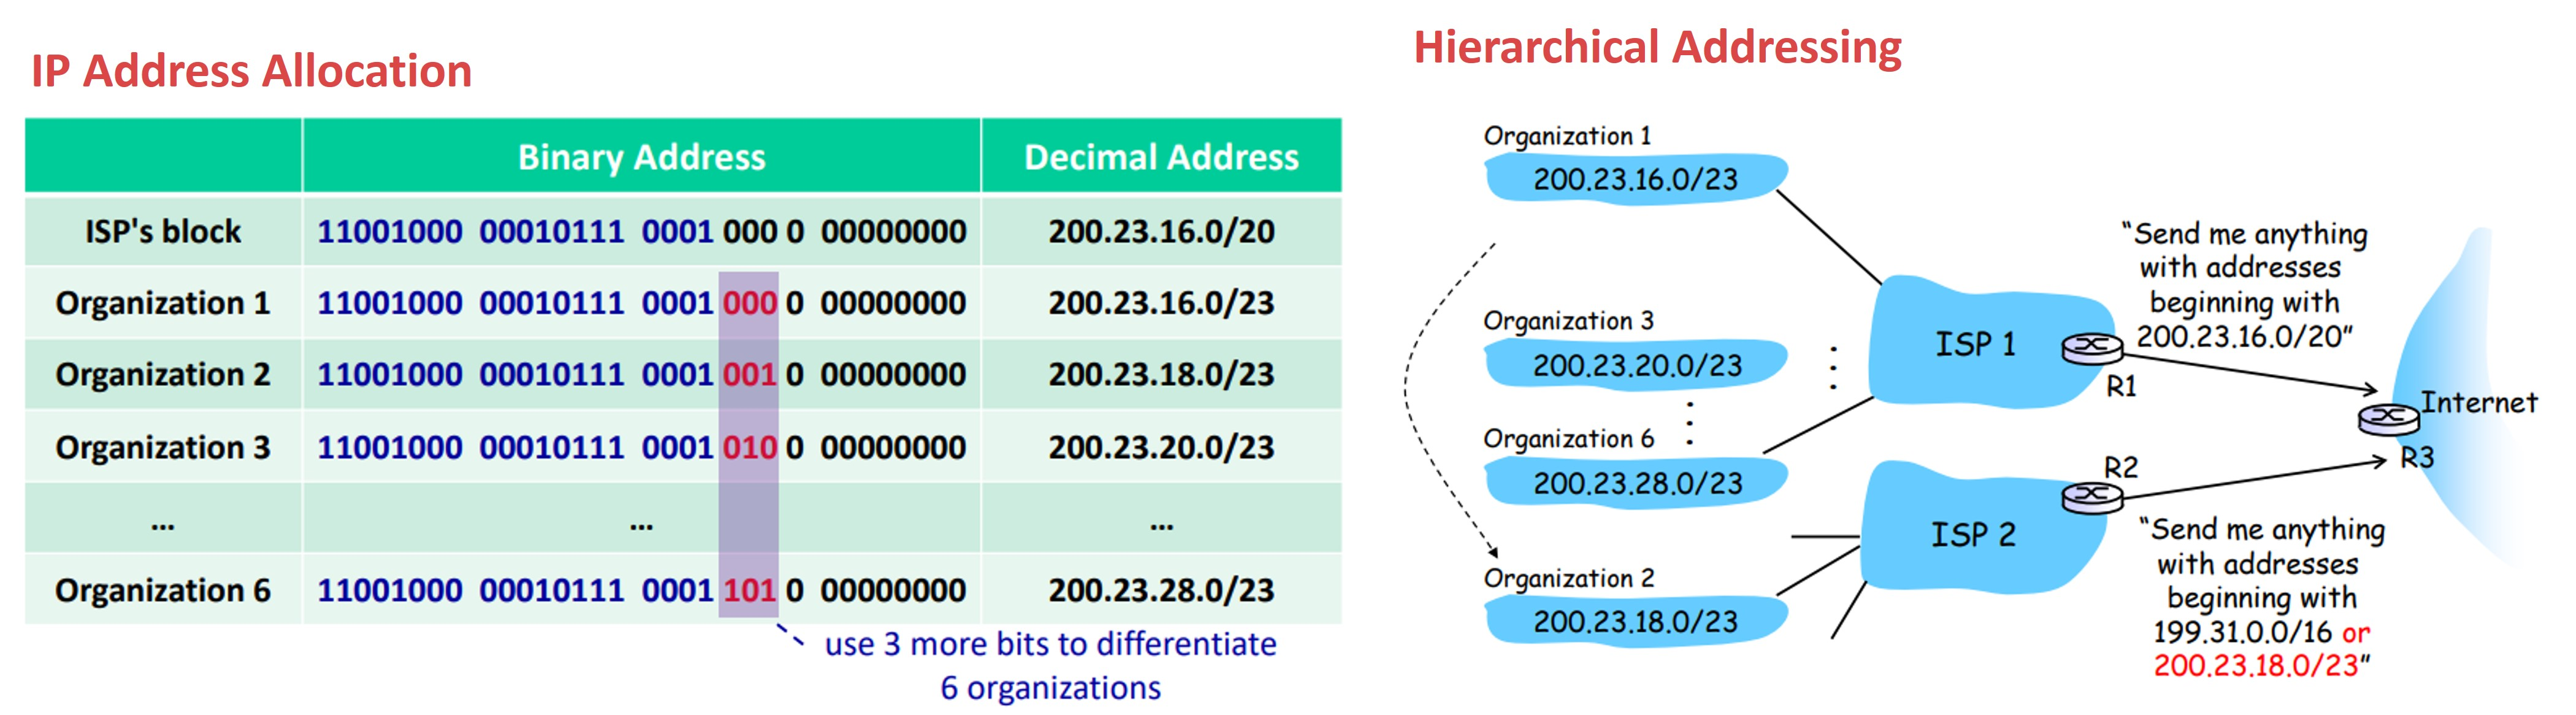
\includegraphics[width=1\linewidth]{IPaddressHA}}
\item \textbf{Longest Prefix Match}: Choose one with longer match. If IP addrr matches all 23 bits for org, packet forwarded, else forwarded to latter.
\end{itemize}

\subsubsection{Network Address Translation (NAT)}
\begin{itemize}
\item Map IP addr space by modifying network addr info in packets IP header through traffic routing device. NAT Routers must:
\item \textbf{Replace} \underline{(source IP address, port \#)} of every outgoing datagram to \underline{(NAT IP address, new port \#)}, \textbf{Remember} (in NAT translation table) the mapping and \textbf{Replace} destination fields of every incoming datagram with that stored in NAT translation table.
\item \textbf{Benefits}: Single public IP for NAT router allows multiple private IP address. Change (private IP) addr of hosts in local network without notifying outside world.
\item ISP change w/o changing local host addresses in local network.
\item Hosts inside local network not explicitly addressable or visible by outside world (security plus).
\medskip
\centerline{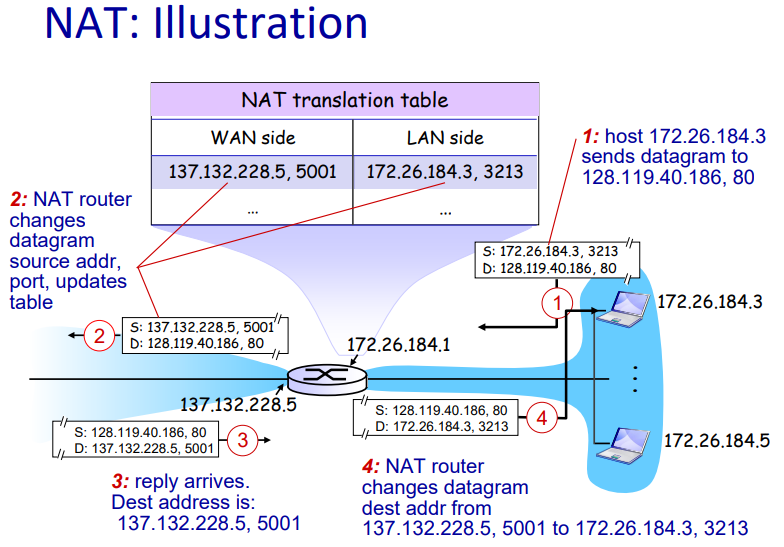
\includegraphics[width=0.85\linewidth]{nat}}
\end{itemize}

\subsubsection{Routing Algorithms}
\begin{itemize}
\item The Internet as \textbf{“network-of-networks”}, hierarchy of \textbf{Autonomous Systems} (AS), e.g., ISPs, each owns routers and links.
\item Due to size and decentralized administration of Internet, routing is done hierarchically.
\item \textbf{Intra-AS routing}: Finds good path btwn two routers within AS. Commonly used protocols: RIP, OSPF
\item \textbf{Inter-AS routing (not covered)} Handles the interfaces between ASs, standard protocol: BGP.
\end{itemize}


\subsubsection{Intra-AS Routing}
\begin{itemize}
\item Abstractly view a network of routers as a graph, vertices are routers, edges are physical links between routers.
\item Associate cost to each link. (cost = 1, or inversely related to bandwidth, or related to congestion)
\item \textbf{Routing}: find least cost path btwn two vertices in graph.
\item \textbf{Link state Algorithmns}: Centralised routing algo, all routers have complete knowledge of network topology and link costs. Routers periodically broadcast link costs to each other.
\item Use Dijkstra algorithm compute least cost path locally! (using global map).
\item \textbf{Distance vector Algorithms}: Decentralised routing algo, Routers know physically-connected neighbors and link costs to neighbors.
\item Routers exchange “local views” with neighbors, update own “local views”. Iterative computation: Swap local view with direct neighbours, Update own view, Repeat till no further change. 
\end{itemize}

\subsubsection{Distance Vector Algo (Bellman Ford)}
\begin{itemize}
\centerline{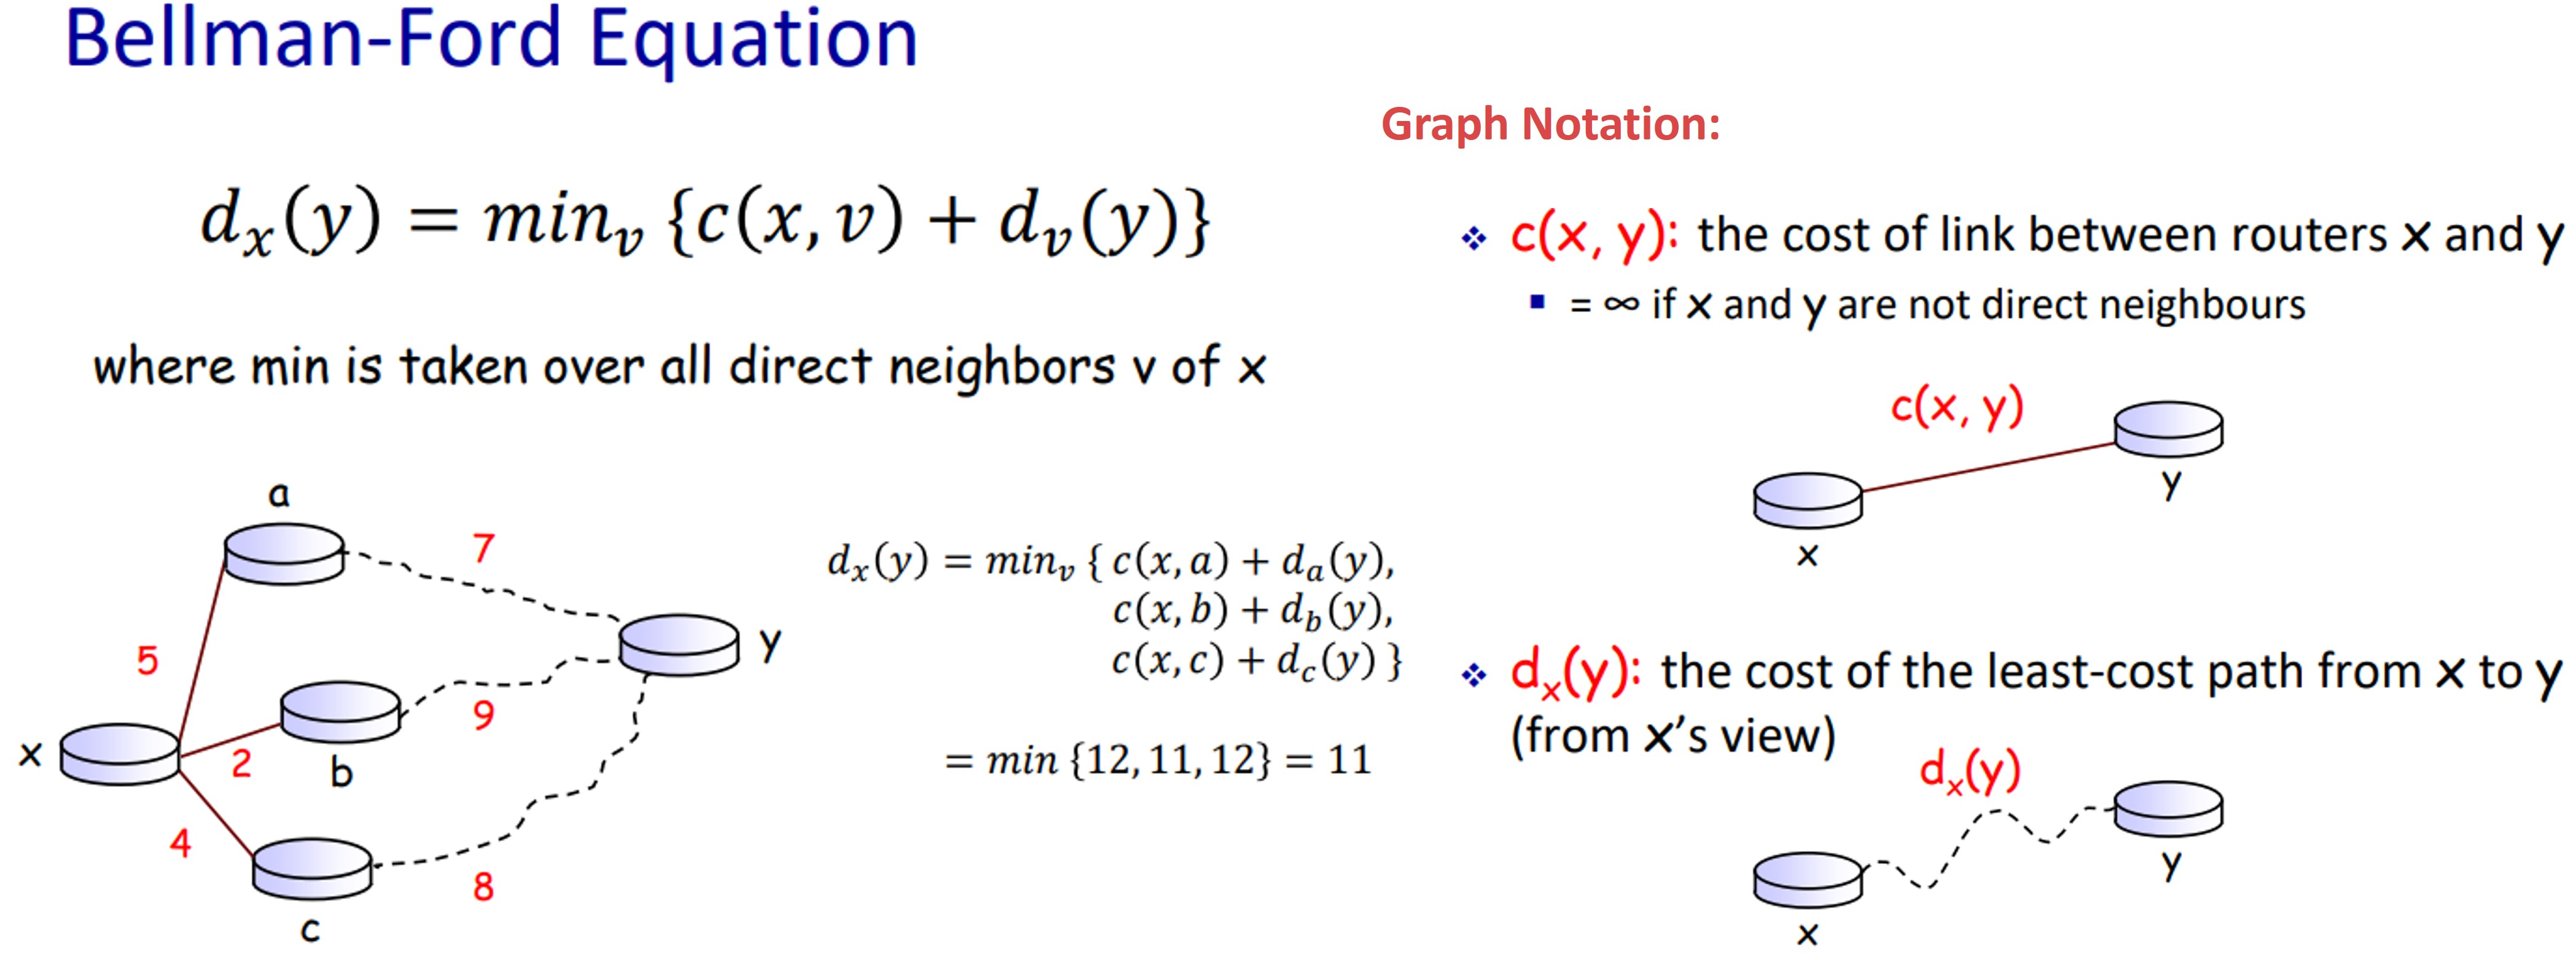
\includegraphics[width=1\linewidth]{bmf}}
\bigskip
\item \textbf{$d_x(y) = min_v \{c(x,v) + d_v(y)\}$}
\item To find \textbf{least cost path}, x needs to know cost from each of its direct neighbour to y. Each neighbour v sends its distance vector (y, k) to x, telling x that the cost from v to y is k.
\item Every router, x, y, z, sends its distance vectors to directly connected neighbors. When x finds y is advertising cheaper path to z than known, x update distance vector to z accordingly and note down all packets for z should be sent to y. Info used to create forwarding table of x.
\item After every router exchanged several rounds of updates with direct neighbors, all routers will know least-cost paths to all other routers.
\end{itemize}

\subsubsection{RIP (Routing Information Protocol)}
\begin{itemize}
\item \textbf{RIP} implements the DV algorithm. Uses hop count as the cost metric (insensitive to network congestion).
\item Exchange routing table every 30 seconds over UDP port 520.
\item “Self-repair”: if no update from a neighbour router for 3 minutes, assume neighbour failed.
\end{itemize}


\subsubsection{Internet Protocol (IP): IPv4}
\begin{itemize}
\medskip
\centerline{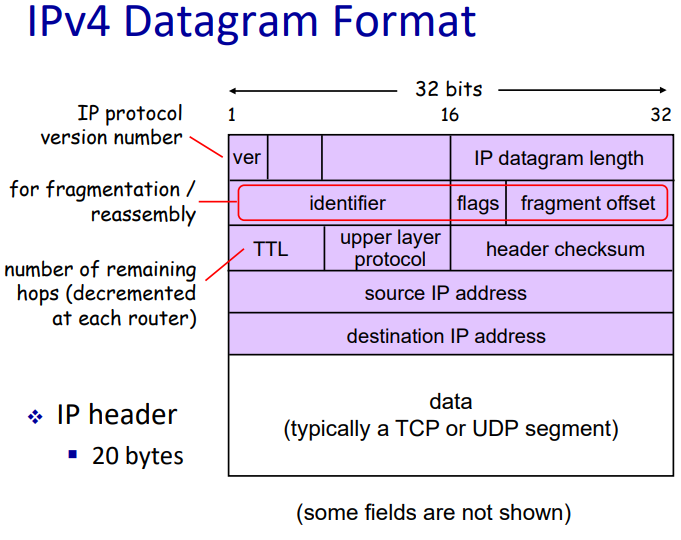
\includegraphics[width=0.9\linewidth]{ipv4datagram}}
\item Length: of IP datagram + 20b header. Identifier, flags, fragment offset: support fragmentation \& reassembly
\item TTL: Prevent infinite circulation. Upper layer protocol: Only used at final dest, determine if UDP/TCP (for Internet). Checksum also uses 1s complement.
\item \textbf{IPv6}: 40b header with 128b IP addr.
\end{itemize}

\subsubsection{IP Fragmentation \& Reassembly}
\begin{itemize}
\item Different links, different MTU (Max Transfer Unit, max amt of data link-level frame can carry).
\item “Too large” IP datagrams may be fragmented by routers. \\
\centerline{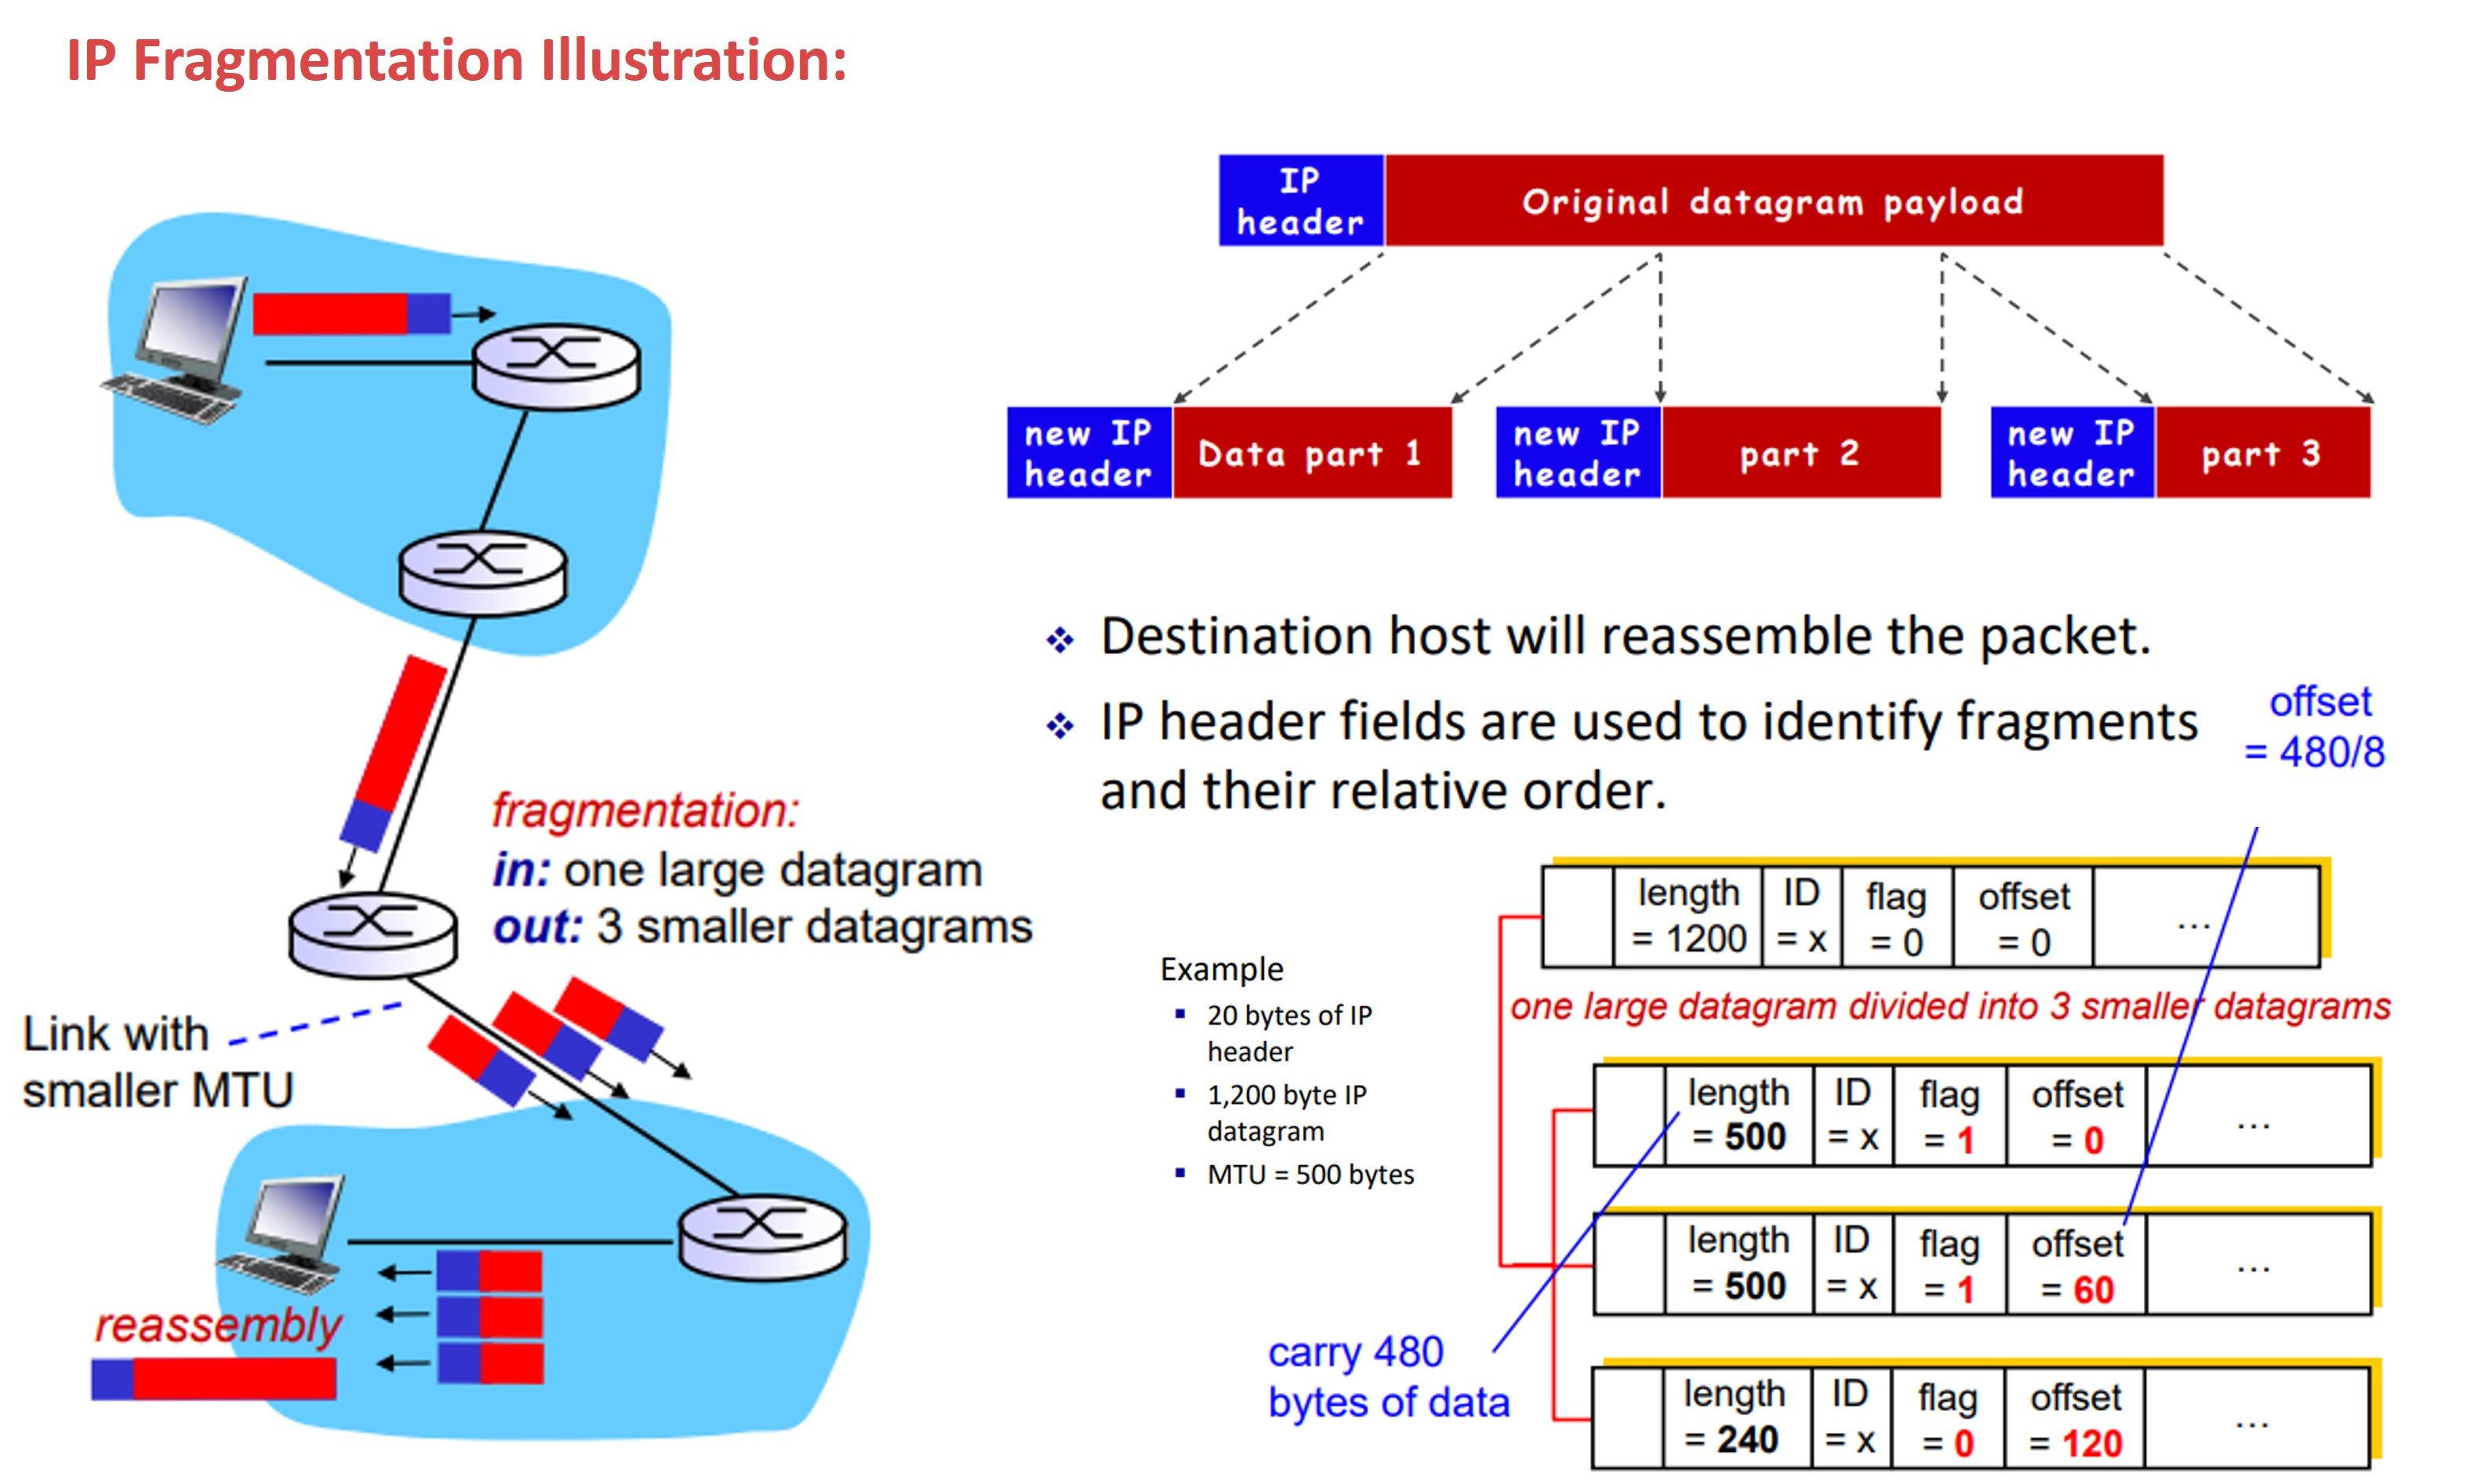
\includegraphics[width=0.9\linewidth]{ipfragmentation}}
\medskip
\item \textbf{Flag}(frag flag) is set to 1 if next fragment from same segment, 0 if this is the last fragment.
\item \textbf{Offset} is in expressed in unit of 8-bytes
\end{itemize}

\subsubsection{Internet Control Message Protocol}
\begin{itemize}
\item \textbf{ICMP}: used by hosts \& routers to communicate network-level information.
\item \textbf{Error reporting}: unreachable host / network / port / protocol.
\item Echo request/reply (used by ping).
\item ICMP messages carried in IP datagrams, ICMP header starts after IP header.
\medskip
\centerline{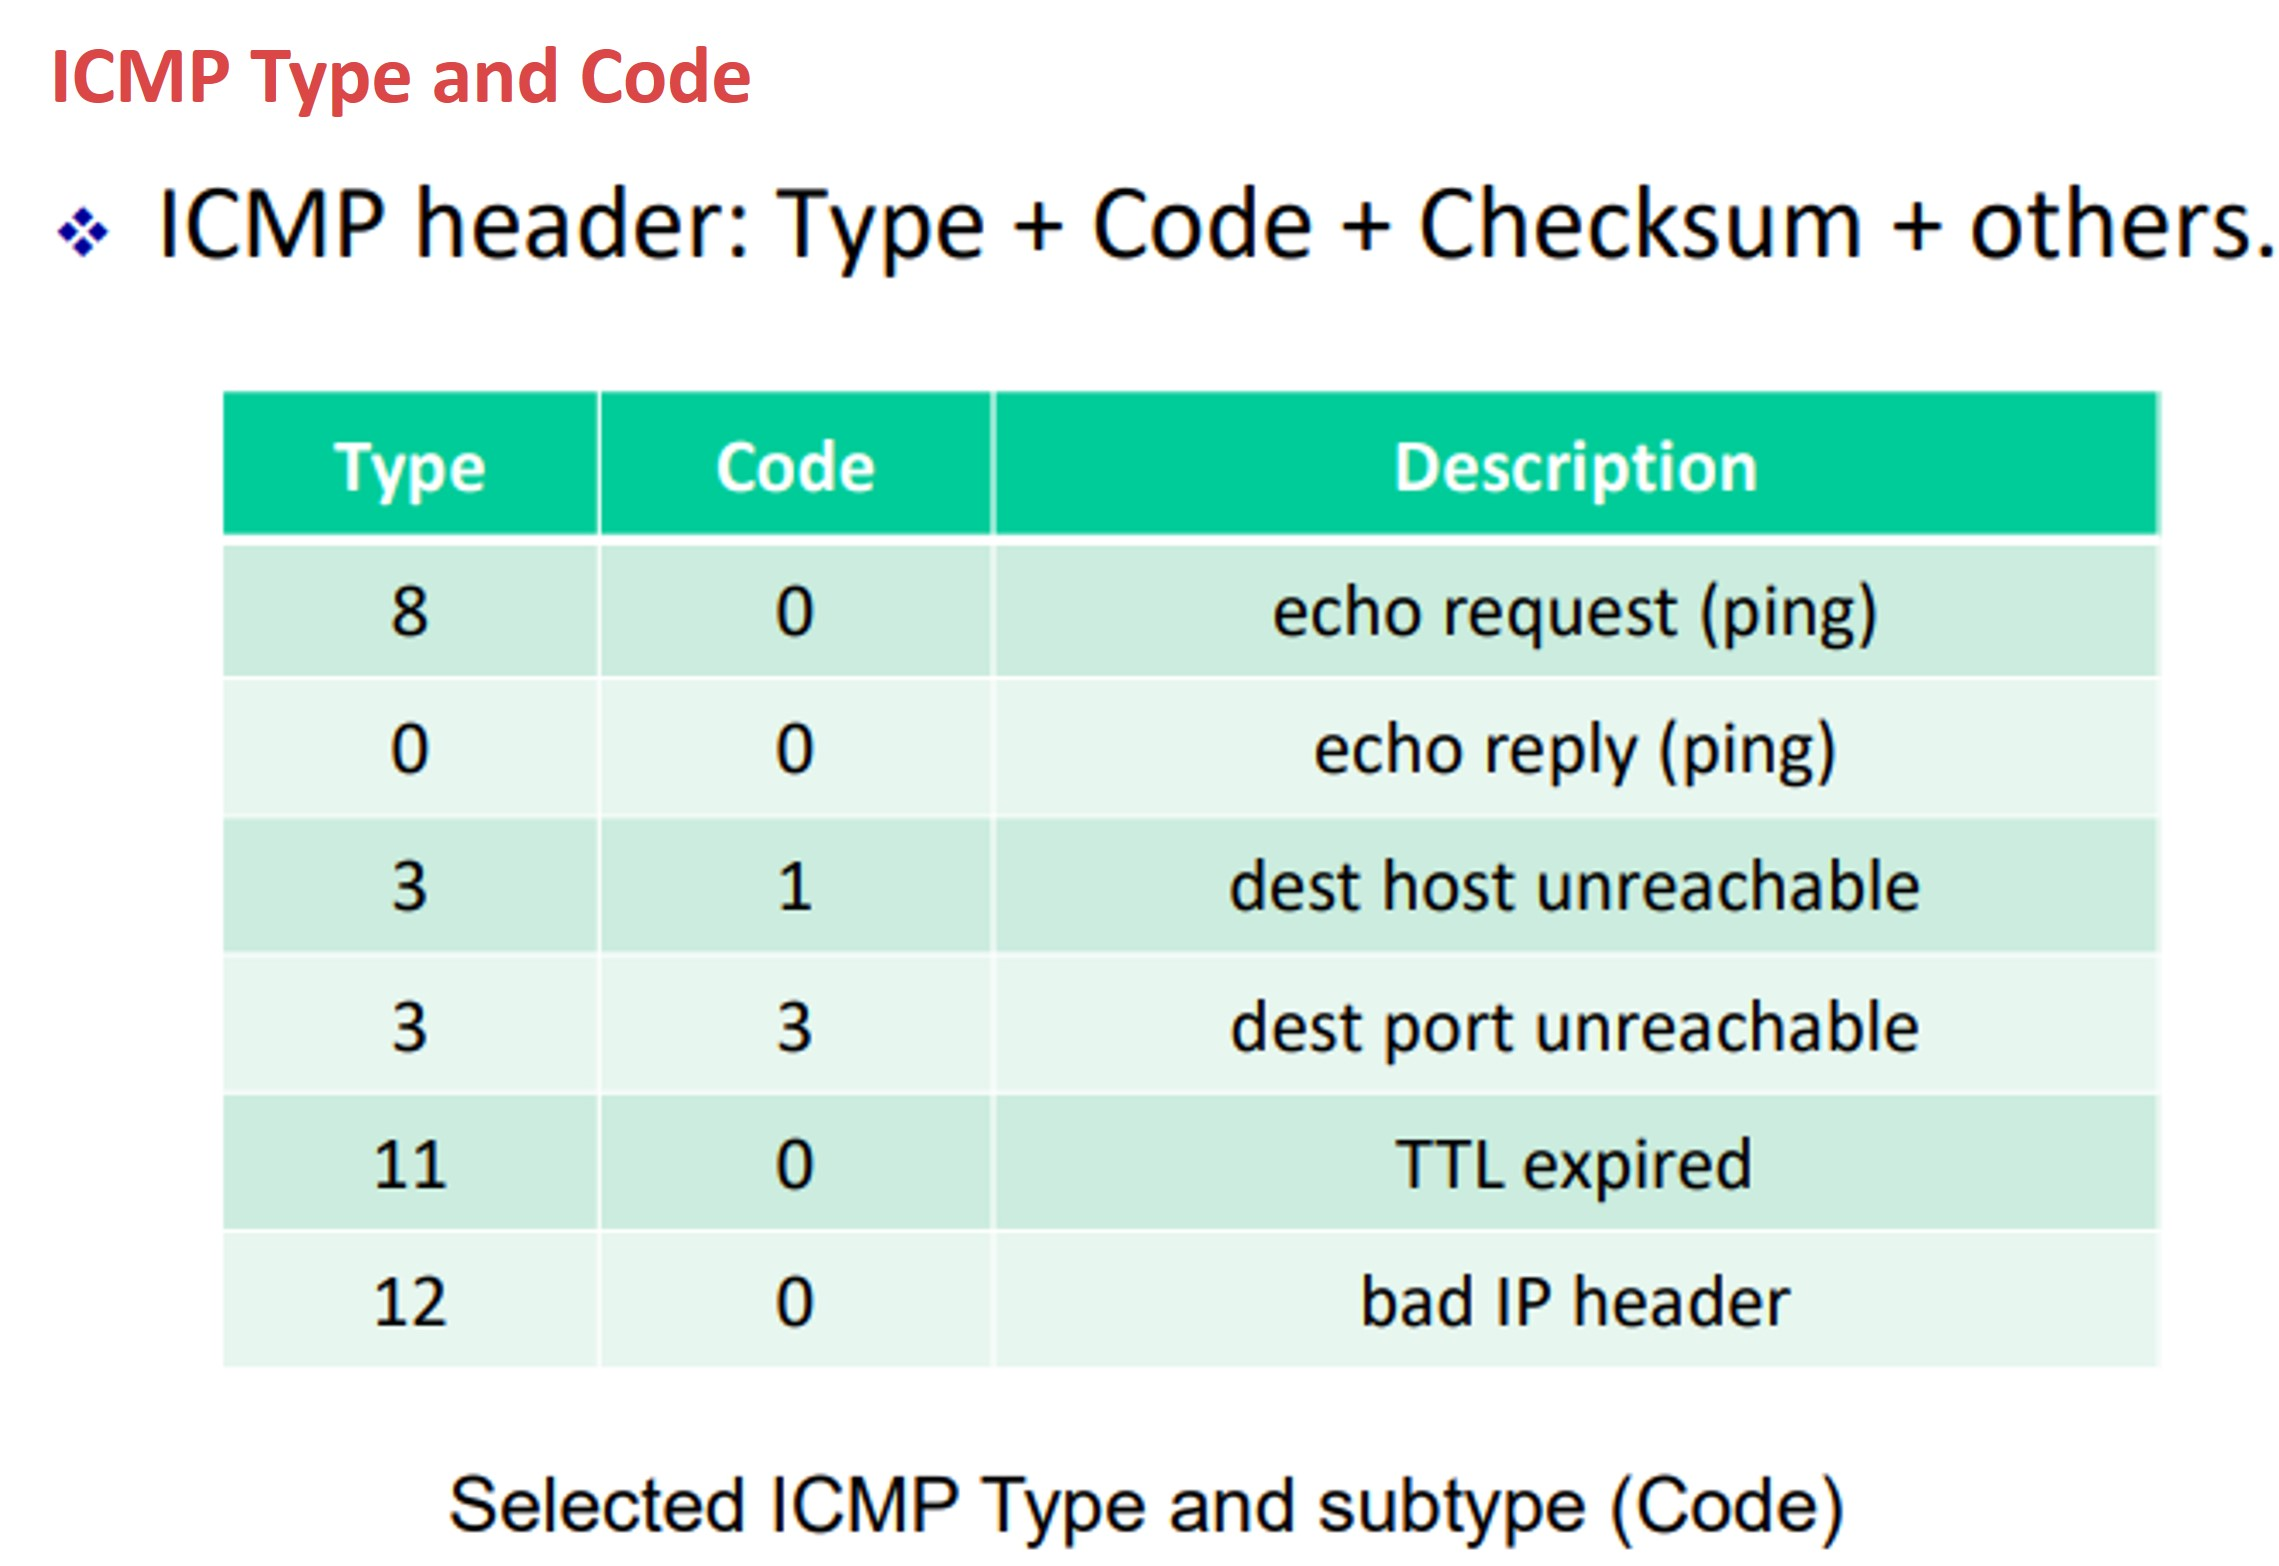
\includegraphics[width=0.7\linewidth]{icmp}}
\end{itemize}

\vfill \null
\columnbreak

\section{5. Link}
\begin{itemize}
\item \textbf{Link Layer}: Concerned about electronics of sending and receiving binary data over a communication channel.
\item \textbf{Communication Channel}: transmission medium of data signals (e.g. copper wire, satellite, optical fiber)
\item \textbf{Node}: Devices exchanging data. (E.g. hosts, routers).
\item \textbf{Link:} Comm. channels that connect adjacent nodes.
\end{itemize}

\subsubsection{Connecting N nodes via cable}
\begin{itemize}
\item \textbf{Aim}: Send data between N nodes via cable.
\item Interconnect N nodes directly: Each link needs to be addressed, N-1 Links needed, does not scale.
\item Interconnect via broadcast link: Each link needs to be addressed, need to define protocol, need to handle errors.
\item Protocol: Framing, Link Access Control. Errors: Detection, Reliability.
\end{itemize}
\smallskip
\centerline{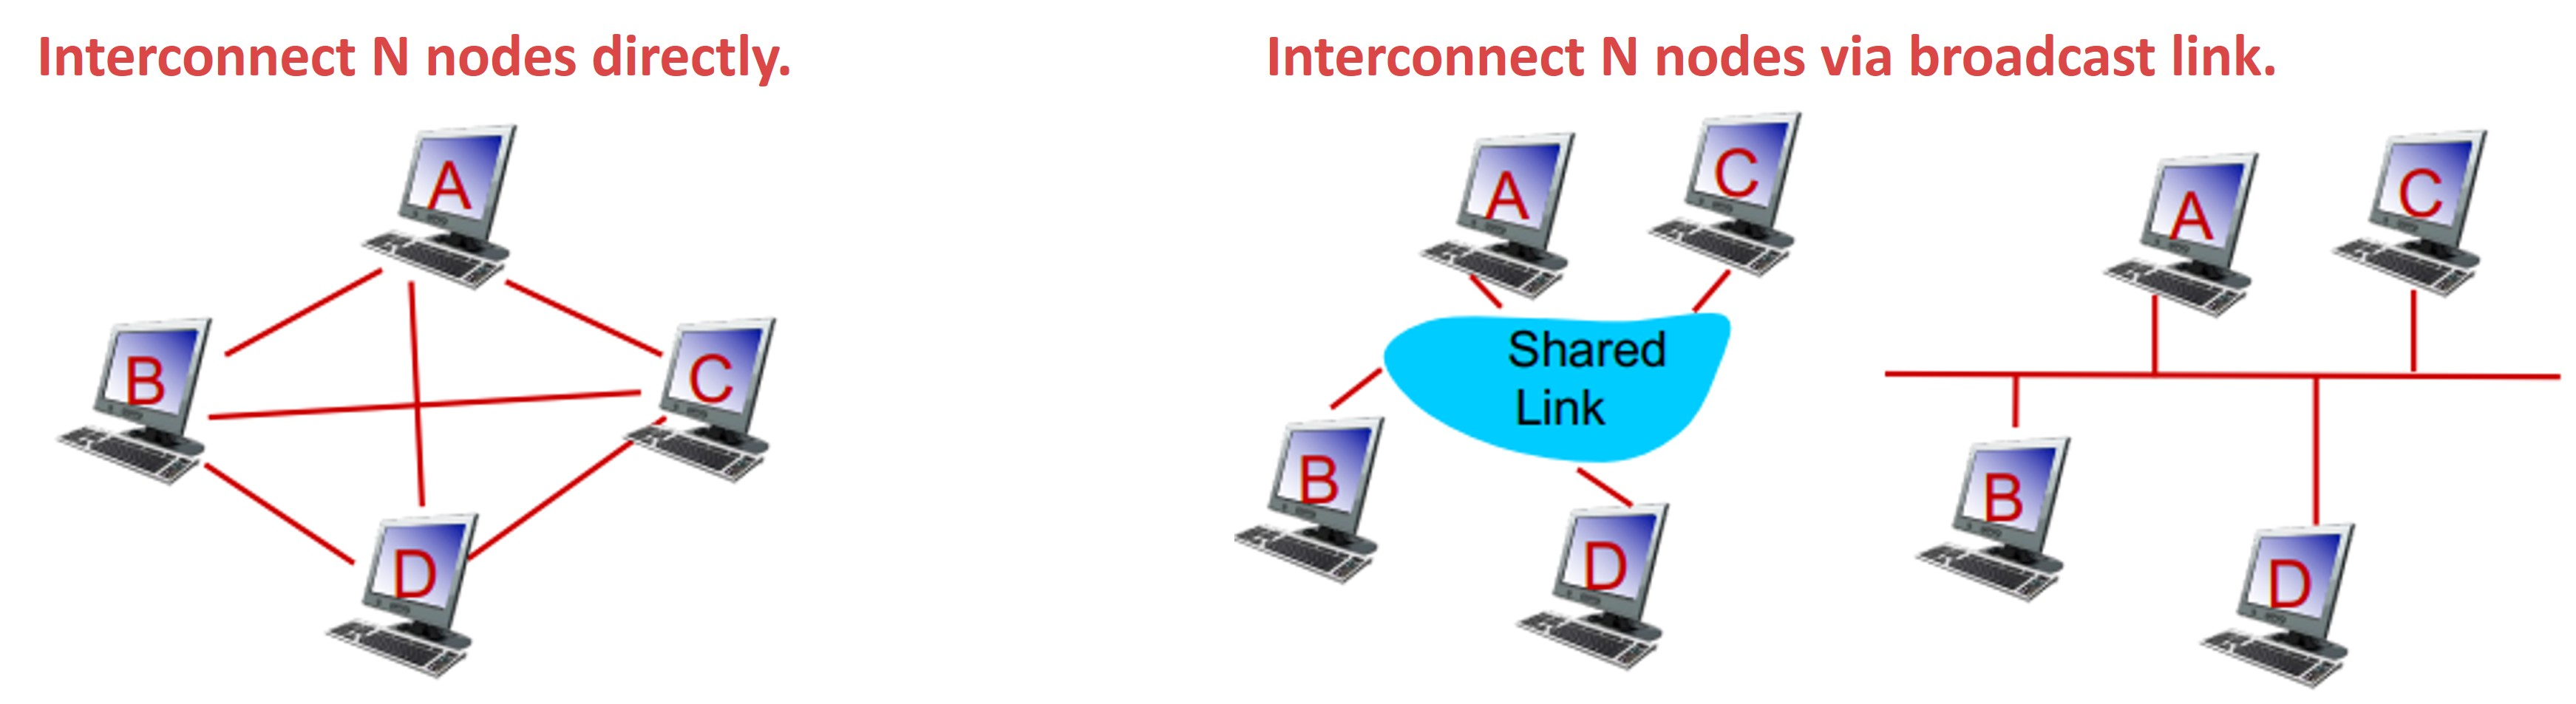
\includegraphics[width=1\linewidth]{interconnectNodes}}

\subsection{Link Layer}
\begin{itemize}
\item  \textbf{Link layer} sends datagram between adjacent nodes (hosts or routers) over a single link. Responsible for transfer of datagram from one node to \underline{physically} \underline{adjacent} node over link. 
\item \textbf{Frames (layer 2 packet)}: IP datagrams are encapsulated in link-layer \textbf{frames} for transmission.
\item \textbf{Protocols}: Different link-layer protocols may be used on different links, each protocol may provide a different set of services.
\end{itemize}

\subsection{Link Layer Services}
\begin{itemize}
\item \textbf{Framing}: Encapsulate datagram into frame, adding header and trailer.
\item \textbf{Link access control}: When multiple nodes share a single link, need to coordinate
 which nodes can send frames at a certain point of time.
\item \textbf{Error detection}: Errors are usually caused by signal attenuation or noise. Receiver detects presence of errors, and  may signal sender for retransmission or simply drops frame.
\item \textbf{Error correction}: Receiver identifies and corrects bit error(s) without resorting to retransmission.
\item \textbf{Reliable delivery}: Seldom used on low bit-error link (e.g., fiber) but often used on error-prone links (e.g., wireless link).
\end{itemize}

\subsection{Network Adapter}
\begin{itemize}
\item \textbf{network adapter}, aka network interface card (NIC), is a single, special-purpose chip that implements the link-layer services above. (e.g. Ethernet card, Wifi Adapter). 
\item Semi-autonomous, implementing both link \& physical layers. Many services implemented in hardware.
\end{itemize}

\subsection{Error Detection and Correction Techniques}
\begin{itemize}
\item \textbf{EDC}: Error Detection and Correction Bits.
\item \textbf{D}: Data protected by error checking, may include header.
\item Larger EDC fields added to link layer frame yields better detection (and correction), but larger overhead.
\item \textbf{Common error detection schemes}: Checksum (used in TCP/UDP/IP), Parity checking, CRC (link layer). 
\item \textbf{Checksum review}: treate segment contents as 16 bit int sequences, get 1s complement of sum of segment contents.
\end{itemize}

\subsubsection{Parity Checking}
\begin{itemize}
\item \textbf{Single Bit Parity}: 1 parity bit for the data. \\
– \textbf{Even Parity Scheme}:  Choose the bit to make the total number of 1s even. \\
– \textbf{Odd Parity Scheme}: Same but we make the number odd.
\item Single bit parity can detect odd number of single bit errors, but cannot detect even single bit errors. 
\item Errors often clustered together in ``bursts'', probability of undetected errors in a  frame can approach 50\%.

\item \textbf{Two-Dimensional Parity}: Divide the datainto rows and columns, and repeat the above but
have parity bits for each column and each row. \\
– Can detect and correct single bit errors in data. \\
– Can detect two-bit errors.
\end{itemize}
\medskip
\centerline{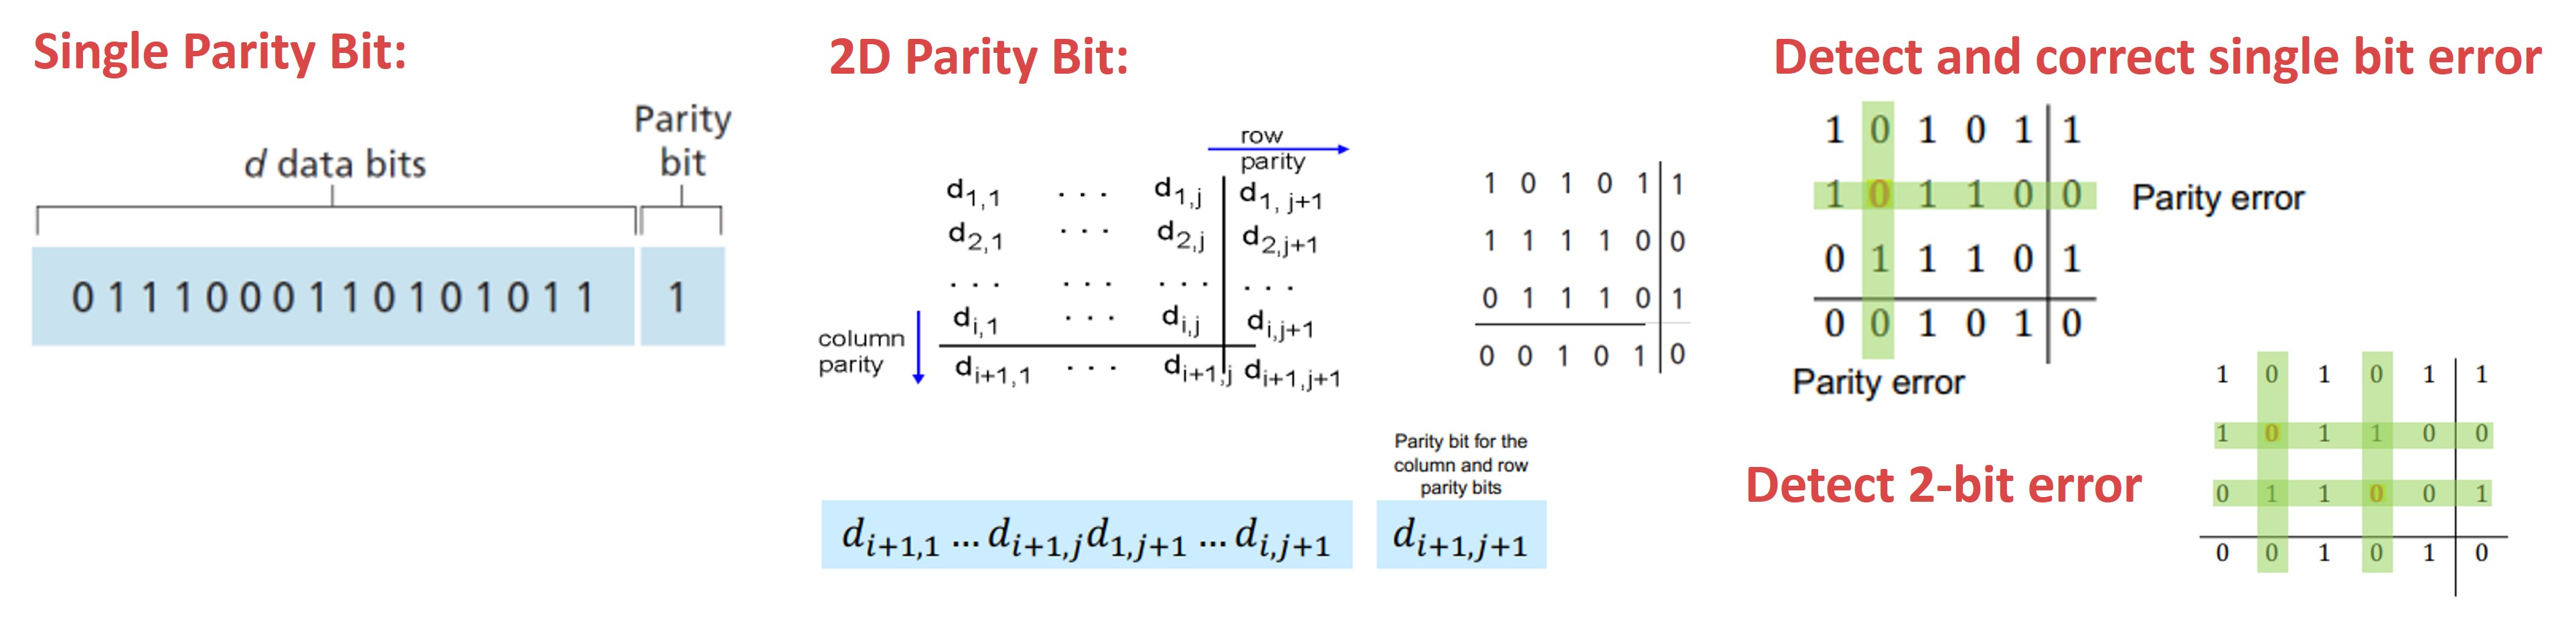
\includegraphics[width=1\linewidth]{paritybit}}

\columnbreak

\subsubsection{Cyclic Redundancy Check}
\begin{itemize}
\item ``Long division'' but with division being replaced by a bitwise XOR operation. 
\item Generally done by hardware, so very fast.
\item \textbf{D: d-bit data}, which is also the dividend.
\item \textbf{G: Generator of r + 1 bits}, which is also the divisor.
\item \textbf{R: r-bit CRC}, which is also the remainder.
\item The resultant $d + r$ bits is “divisible” by G, so the receiver can check for a zero remainder.
\item Can detect all odd number of single bit errors.
\item CRC of r bits can detect all burst errors of less than $r + 1$ bits, burst errors greater than $r$ bits with probability $1 - 0.5^r$. Aka polynomial code.
\end{itemize}
\centerline{\includegraphics[width=1\linewidth]{crc}}

\subsection{Multiple Access Links and Protocols}
\begin{itemize}
\item \textbf{Multiple Access Protcols:} Categorisable into three broad classes: Random Access, ``Taking Turns'', Channel Partitioning.
\item \textbf{Ideal MAP}: Collision free, Efficient, Fairness, Fully Decentralized.
\item Additionally, coordination about channel sharing must use channel itself (no out-of-channel signalling).
\end{itemize}

\subsubsection{Types of Network Links (2)}
\begin{itemize}
\item \textbf{Point-to-point link}: Sender and receiver connected by a dedicated link. No need for multiple access control.
\item \textbf{Broadcast link:} Multiple nodes connected to same shared broadcast channel. When any one node transmits a frame, all other nodes in the channel receives a copy. We need a Multiple Access Protocol to prevent frame collisions.
\end{itemize}

\columnbreak

\subsubsection{Multiple Access Protocols}
\subsubsection{Channel Partitioning Protocols}
\begin{itemize}
\item \textbf{TDMA: Time Division Multiple Access}
\item Each node gets fixed length time slot (time frame), where {length $=$ frame transmission time}. This repeats in rounds. Unused slots go idle.
\item \textbf{FDMA: Frequency Division Multiple Access}
\item Channel spectrum is divided into frequency bands, and each node is assigned one band. Bandwidth has thus decreased, thus transmission is slower. Unused transmission time in frequency bands go idle.
\item Both TDMA and FDMA: Collision Free, Inefficient, Perfectly Fair and fully Decentralized.
\end{itemize}
\smallskip
\centerline{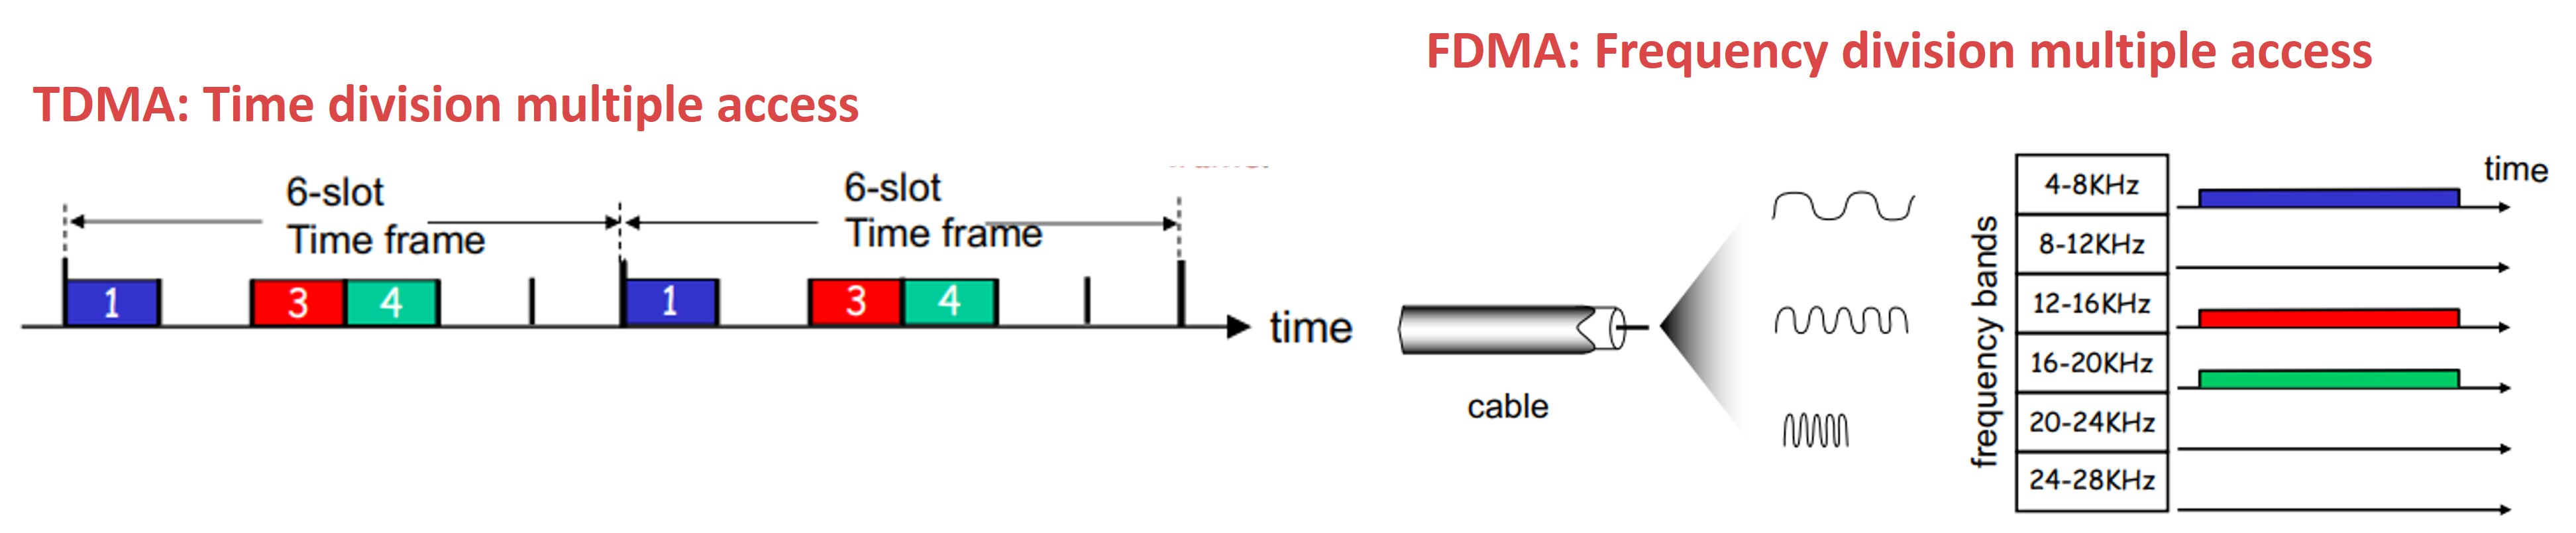
\includegraphics[width=1\linewidth]{tdmafdma}}

\subsubsection{Taking Turns Protocols}
\begin{itemize}
\item \textbf{Polling} 
\item A master node invites each of the other nodes (slaves) to transmit in turns. Minor polling overhead. A single point
of failure, which is the master node.
\item \textbf{Token Passing (Token Ring) / Round Robin}
\item Control token is passed from one node to the next sequentially. There is overhead for the token and single point of failure as well, which is the token.
\item Even if only a few of the nodes have data to send, it can still be quite efficient.
\end{itemize}

\subsubsection{Random Access Protocols}
Generally these protocols specify how to detect and recover from collisions (When two or more transmitting nodes). \\
Thus, no need for centralised coordination, thus no single point of failure.

\subsubsection{Slotted ALOHA}
\begin{itemize}
\item  Assume all frames are of the same size, and split the time into slots of equal length, where length $=$ time to transmit 1 frame $= L (bits)/ R (rate)$.
\item A node will only transmit at the start of a slot.
\item Each node listens to the channel while transmitting. If a collision occurs, it retransmits in each subsequent slot with probability $p$ until success.
\item $p$ depends on network congestion
\item \textbf{Effectiveness}: Not collision free, Efficiency high when only one node is active, but maximum efficiency falls to 37\% when  many active nodes (collision \& empty slots). Perfectly fair and decentralized.
\end{itemize}

\subsubsection{Pure (Unslotted) ALOHA}
\begin{itemize}
\item  Like ALOHA but no slots nor synchronisation, just transmit when there’s a fresh frame.
\item Chance of collision increases, as now it can collide with frames both in front and behind $(t_0 -1, t_0 + 1)$.
\item \textbf{Effectiveness}: Not collision free, Efficiency high when only one node is active, but maximum efficiency falls to 18\% when many active nodes (collision \& empty slots). Perfectly fair and decentralized.
\end{itemize}
\smallskip
\centerline{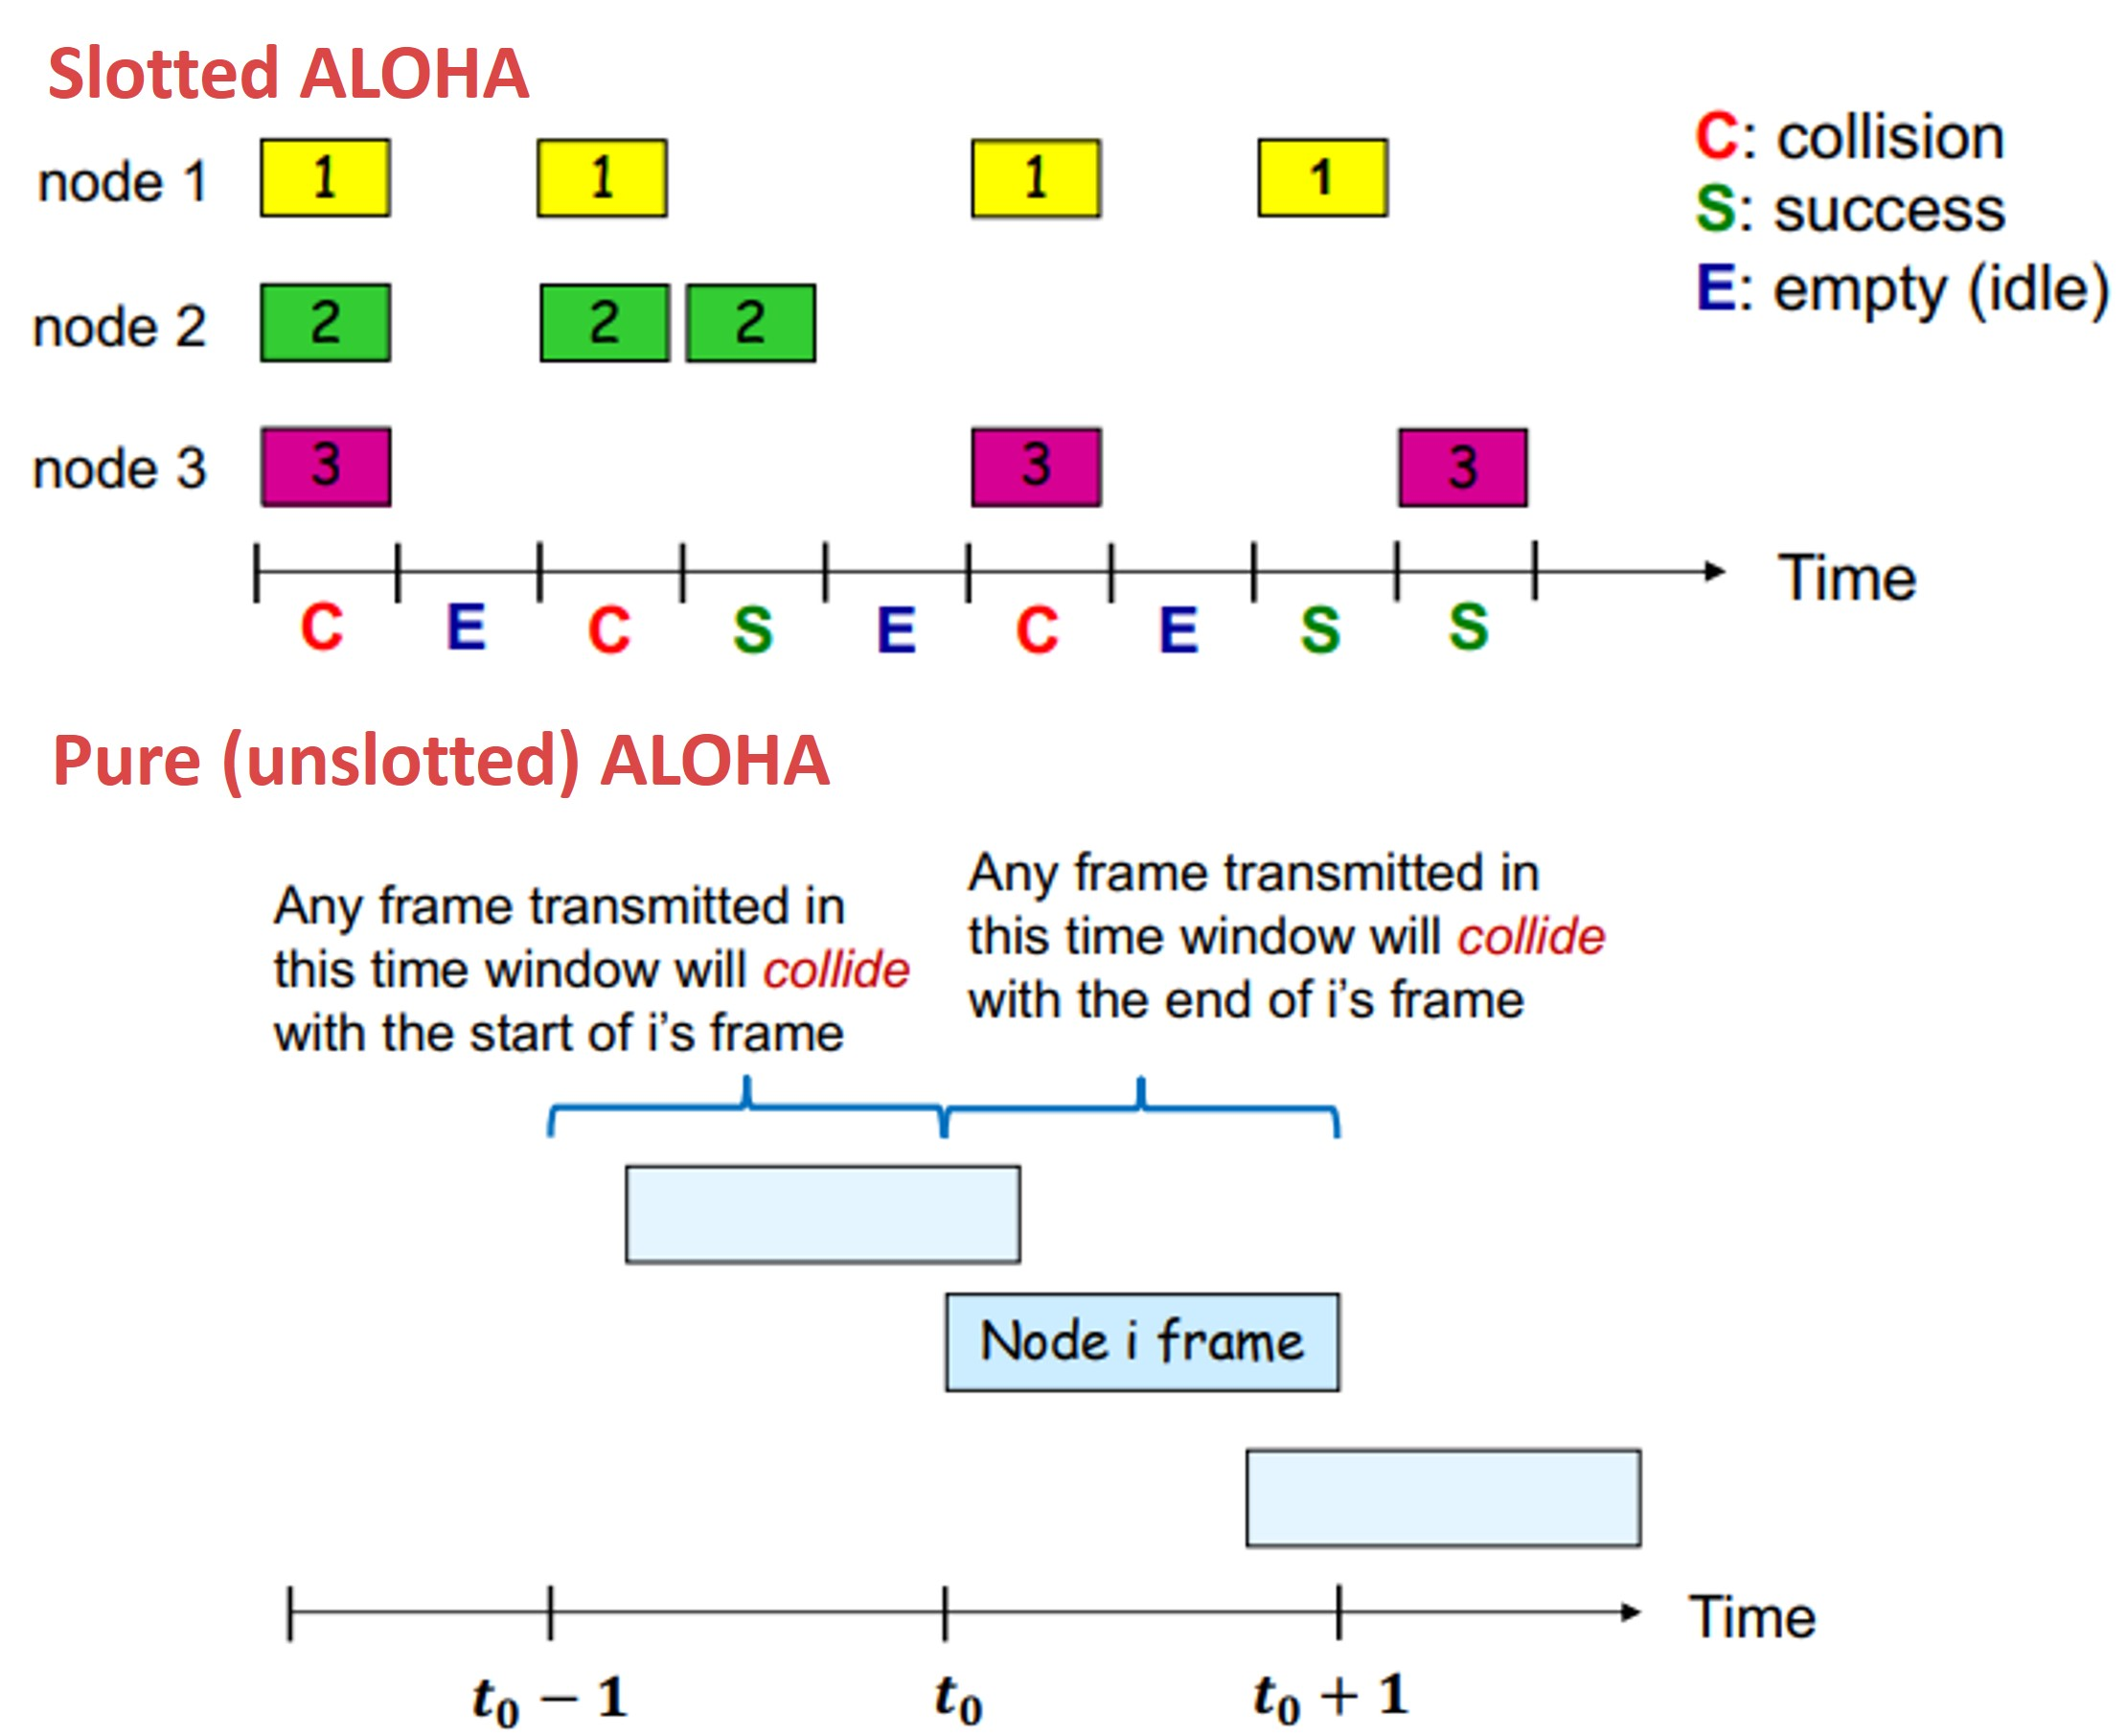
\includegraphics[width=1\linewidth]{aloha}}

\subsubsection{Carrier Sense Multiple Access (CSMA)}
\begin{itemize}
\item Sense if the channel is idle, if so, transmit frame.
\item Still collides when two nodes sense that a channel is idle.
\item Collision: propagation delay, nodes far apart, two nodes may not hear each other's transmission immediately.
\item CSMA transm. does not stop despite collision detection. 
\end{itemize}

\subsubsection{Carrier Sense MA/ Collision Detection (CSMA/CD)}
\begin{itemize}
\item \textbf{Backoff Algorithm}: Same as CSMA except the moment a collision is detected, the node stops transmission.
\item The node then retransmits after some random amount of time. (probability $p$ for each sub. frame until success).
\item \textbf{Binary Exponential Backoff}: More collisions implies heavier load, adapt retransmission attempt to estimated current load. Longer back-off interval with more collisions.
\item After the $m^{th}$ collision, we choose K at random from $0, 1, ... , 2m - 1$, then wait $K * 512$ bit transmission
times before retransmitting.
\item \textbf{Effective:} Both Efficent, Fair, Decentralized, but both CSMA/[CD] not collision free.
\end{itemize}
\centerline{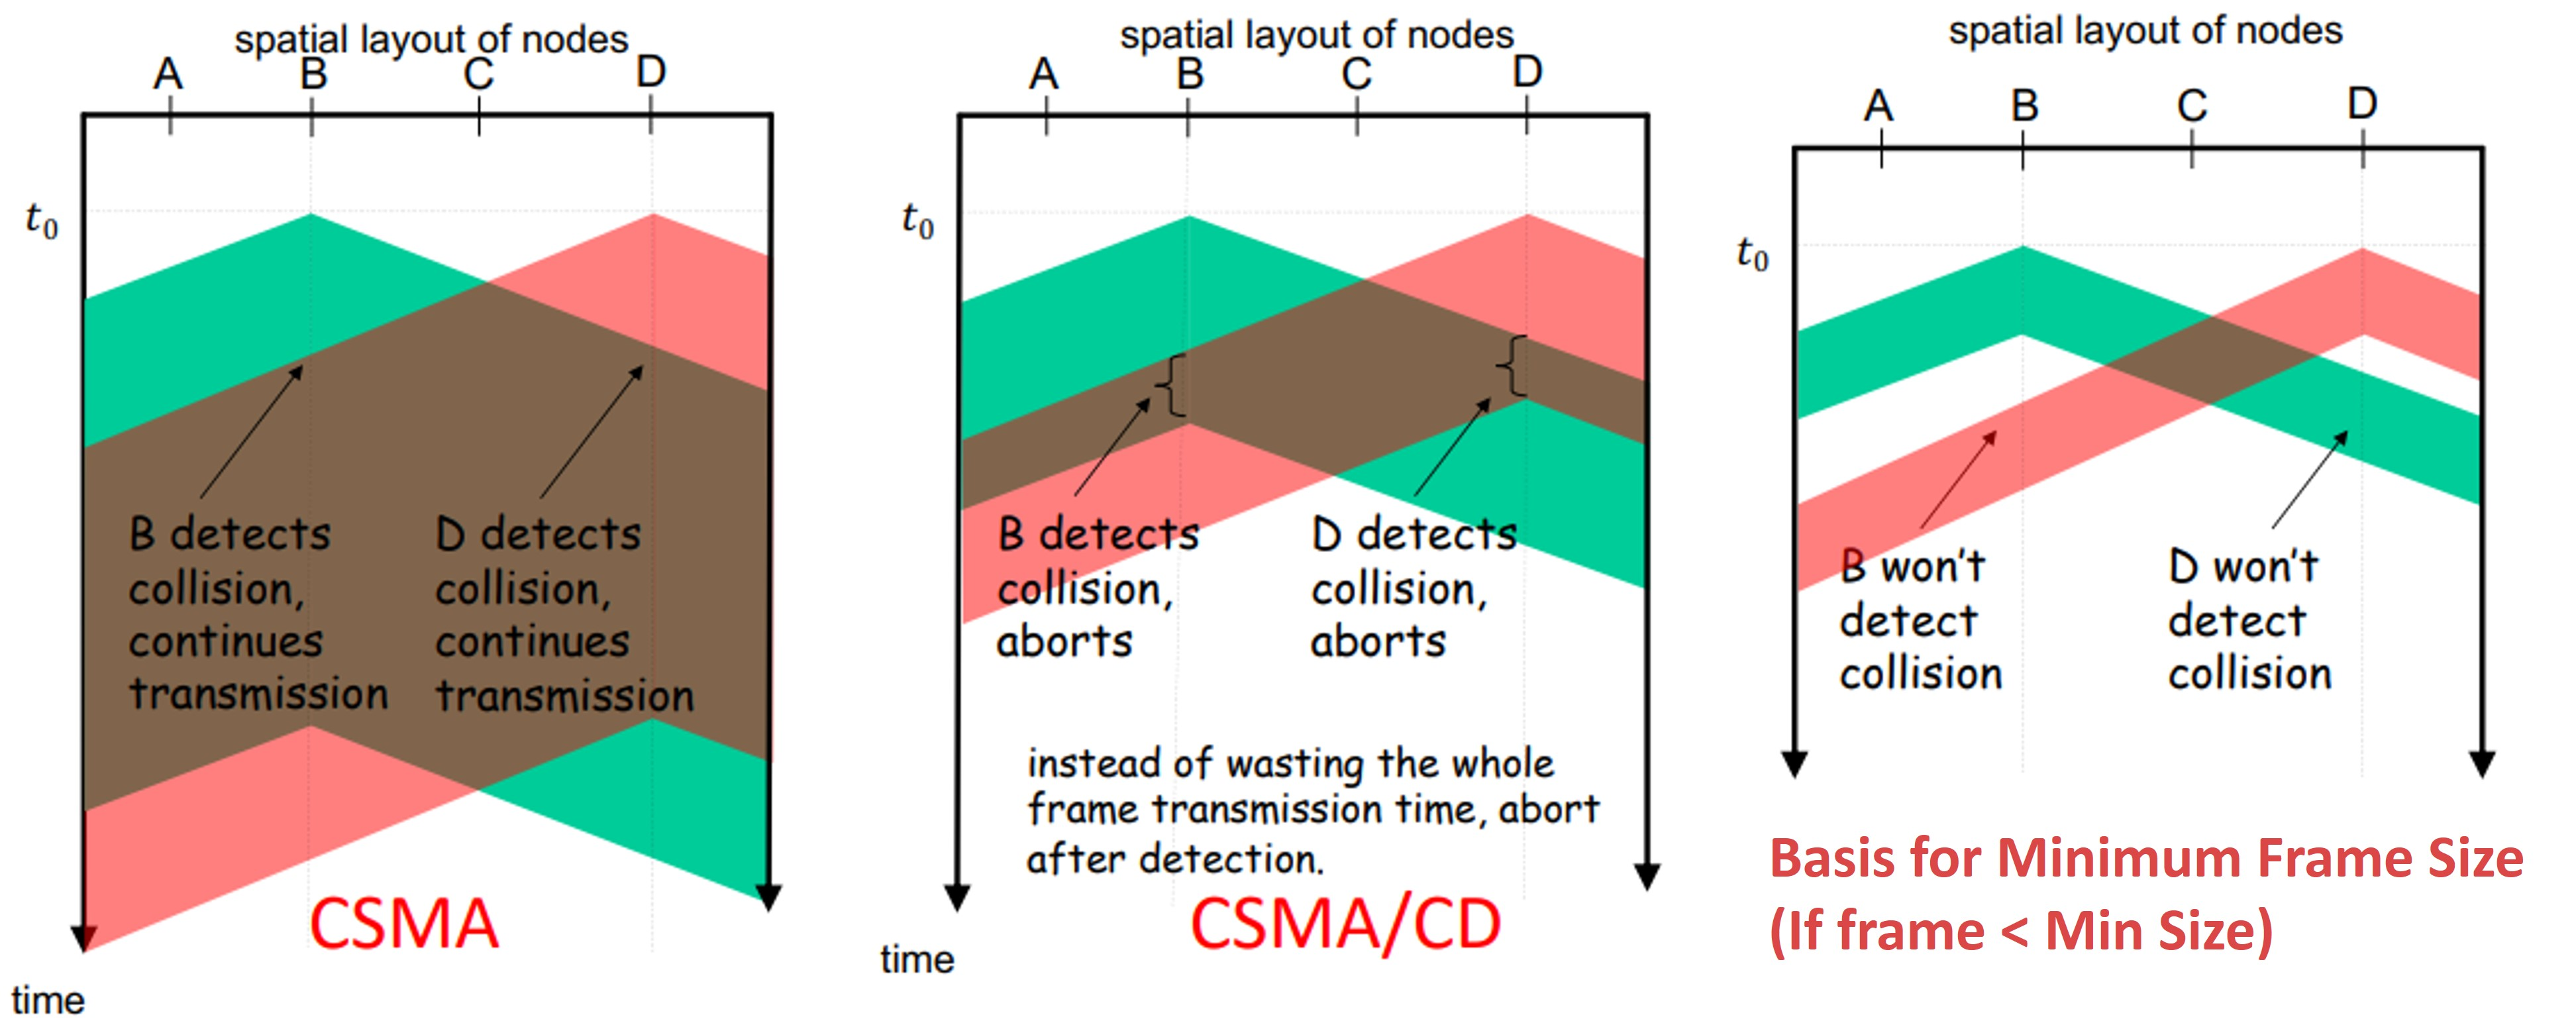
\includegraphics[width=1\linewidth]{csma}}

\subsubsection{Minimum Frame Size}
\begin{itemize}
\item For CSMA and CSMA/CD above, need minimum frame size so that collisions can always be detected. 
\item Ethernet has a minimum size of 64 bytes.
\end{itemize}

\subsubsection{CSMA / Collision Avoidance (CSMA/CA)}
\begin{itemize}
\item Collision detection can be hard for wireless LANs, as energy levels drop too quickly.
\item Hidden Node Problem: When two nodes cannot detect each other but a node in-between encounters a collision.
\item As such, an ACK is required from the receiver as well.
\end{itemize}

\subsubsection{Bit Times}
\begin{itemize}
\item Common unit used in multiple access protocols is bit times. 
\item Bit transmision time, is time taken to transmit 1 bit. 
\item Often, used as such: propagation delay is equals to 800 bit times. This means the propagation delay is equals to the time
it takes to transmit 800 bits onto the link.
\end{itemize}

\null \null \null \null \null \null
\null \null \null \null \null \null

\columnbreak

\subsection{Switched Local Area Networks}
\subsubsection{MAC Address}
\begin{itemize}
\item Every adapter (NIC) has a unique MAC address (aka physical or LAN address).
\item \textbf{MAC}: Media Access Control.
\item Used to send and receive link layer frames, when adapter receives a frame, it checks if the destination MAC address of the frame matches its own MAC address.
\item If yes, adapter extracts enclosed datagram and passes it to the protocol stack.
\item If no, adapter simply discards the frame without interrupting host.
	\begin{itemize}
	\item  \textbf{48 bits:} Burned in NIC ROM (read-only memory), e.g. 5C-F9-DD-E8-E3-D2
	\item \textbf{IEEE}: Administers the MAC address allocation. The first three bytes of the MAC identifies the vendor of the adapter.
	\item If somehow MAC is manually configured to be not unique, and the NICs are on the same subnet, transmission will be severely affected.
	\end{itemize}
\end{itemize}

\subsubsection{Local Area Network (LAN)}
\begin{itemize}
\item  \textbf{LAN} is a computer network that interconnects computers within a geographical area such as 
office building or university campus.
\item Example LAN technologies: IBM Token Ring: IEEE 802.5 standard, Ethernet: IEEE 802.3 standard, Wi-Fi: IEEE 802.11 standard
\end{itemize}
\smallskip

\centerline{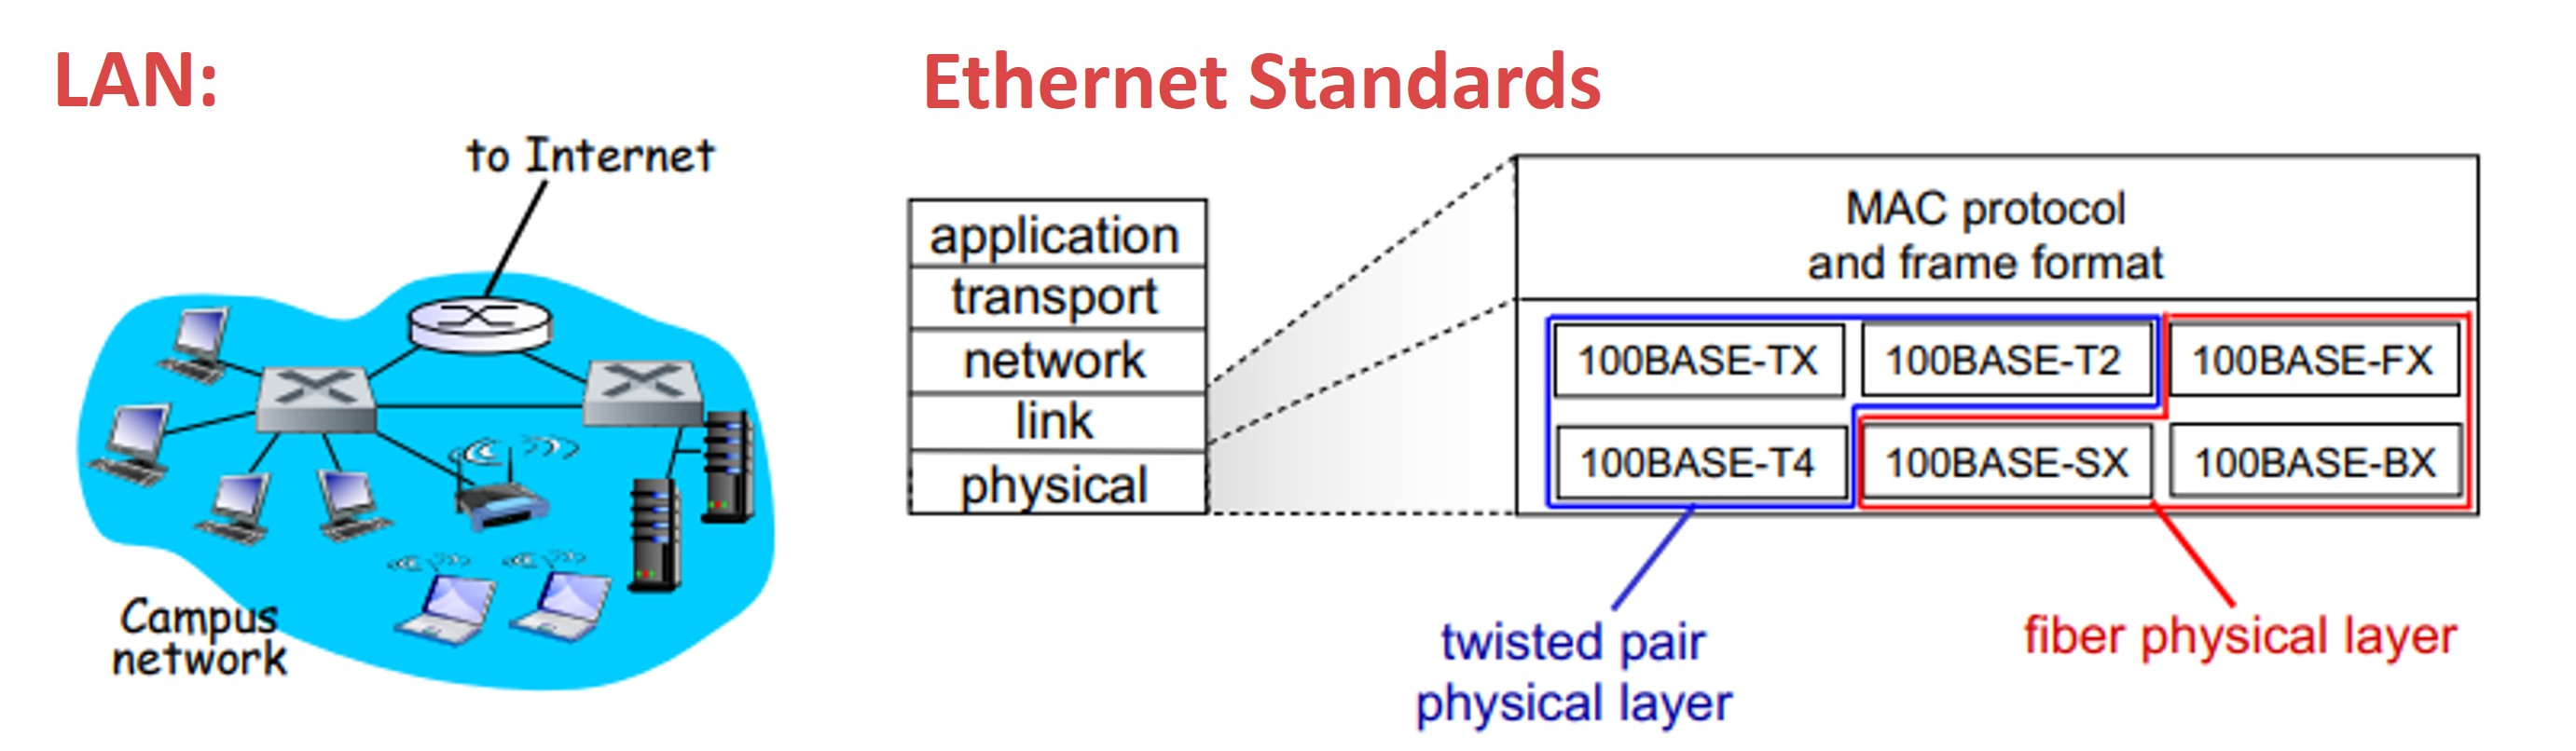
\includegraphics[width=0.8\linewidth]{lanEthernet}}
\subsubsection{Ethernet}
\begin{itemize}
\item \textbf{Ethernet}: “Dominant” wired LAN technology, developed in mid 1970s, Standardized by Xerox, DEC, and Intel in 1978.
\item Simpler and cheaper than token ring and ATM (asynch transf mode).
\item MAC protocol, frame format remain unchanged over years.
\end{itemize}


\subsubsection{Ethernet Frame Structure}
\begin{itemize}
\item Sending NIC (adapter) encapsulates IP datagram in Ethernet frame.
\centerline{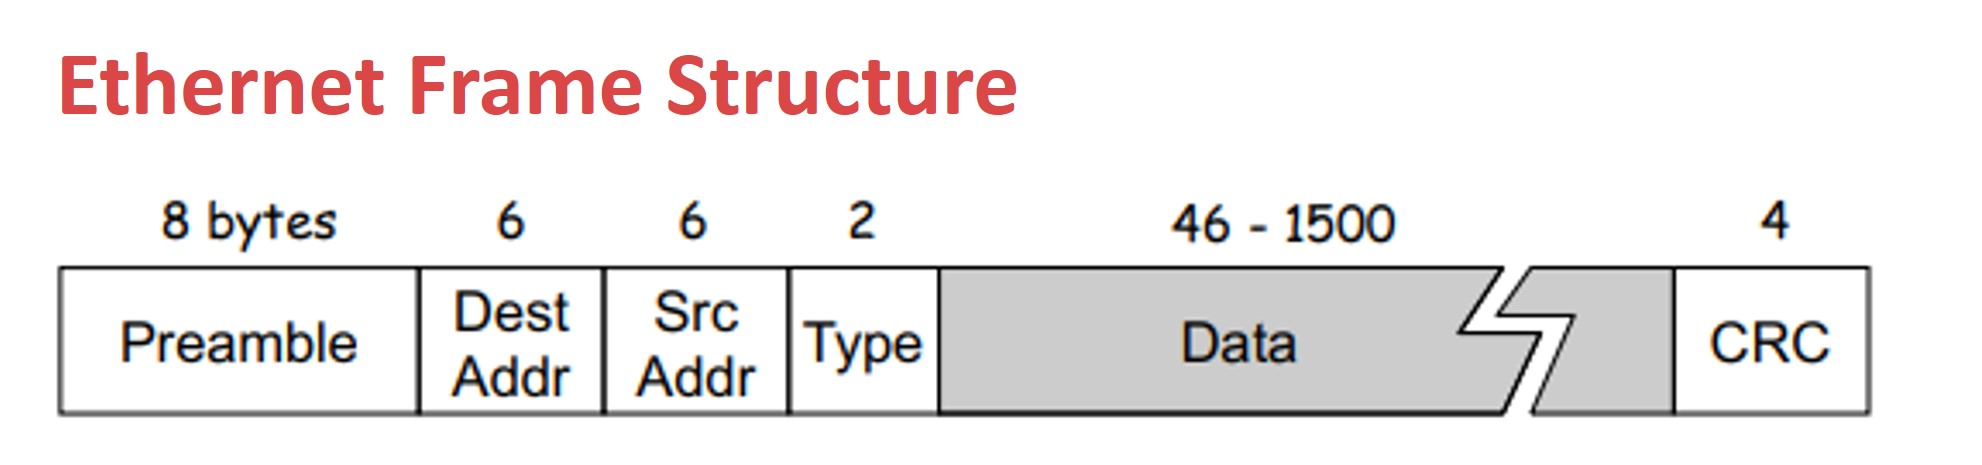
\includegraphics[width=1\linewidth]{ethernetframe}}
\item \textbf{Preamble}:  7 bytes with pattern $10101010$ ($AA_{Hex}$), Followed by 1 byte with pattern $10101011$ ($AB_{Hex}$). Also called “start of frame”. Allows sender and receiver to synchronise clock rates, as alternating bits form a square wave. Lets receiver know how long 1 bit is.
\item \textbf{Source and dest MAC address}: If NIC receives frame with matching \underline{destination address} or with \underline{broadcast address}, passes data in frame to network layer protocol, otherwise, NIC discards frame.
\item \textbf{Data / Payload}: The maximum size is 1500 bytes, which is link MTU mentioned in IP fragmentation. Minimum size is 46 bytes, to ensure that collision will always be detected. 
\item \textbf{CRC}: For corruption detection.
\item \textbf{Type}: Higher level protocol used, usually IP. (others e.g. ARP, AppleTalk), permits Ethernet to multiplex network-layer protocols.
\end{itemize}

\subsubsection{Ethernet Topology}
\begin{itemize}
\item \textbf{Bus Topology}: (broadcast LAN) All nodes are connected and can collide with each other.
\item \textbf{Star Topology}: Switch / Hub in the centre and nodes are connected to that switch. Do not collide with each other.
\end{itemize}

\smallskip
\centerline{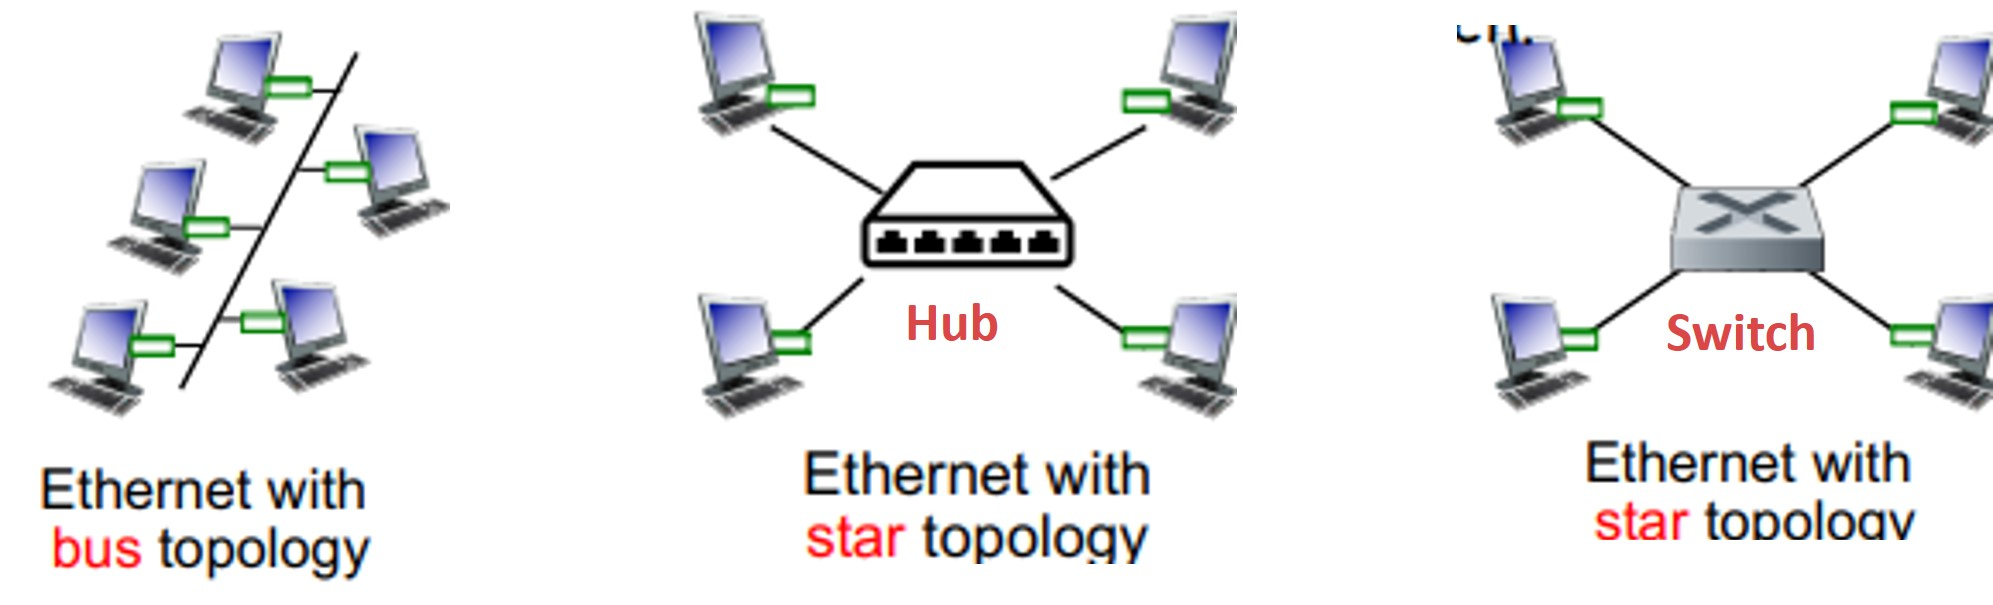
\includegraphics[width=0.8\linewidth]{topo}}

\subsubsection{Ethernet Delivery}
\begin{itemize}
\item \textbf{Connectionless}: No handshaking btwn. sender \& receiver.
\item \textbf{Unreliable}: NIC does not send ACK/NAK. Data in dropped frames recovered only if initial sender uses higher layer rdt (e.g. TCP).
\item \textbf{Ethernet’s multiple access protocol}: CSMA/CD with binary (exponential) backoff.
\end{itemize}

\subsubsection{Ethernet CSMA/CD Algorithm}
\begin{enumerate}
\item NIC receives datagram from network layer, creates frame.
\item If NIC senses that the channel is idle, start frame transmission. Else, wait until idle.
\item If NIC transmits the entire frame without detecting another transmission, NIC is done.
\item If another transmission is detected, NIC aborts and sends a \textbf{jam signal}, tells all other nodes that
a collision has been detected and NIC will be retransmitting.
\item After aborting, NIC enters exponential (binary) backoff, and repeat from step 2
\end{enumerate}



\subsubsection{Ethernet Hub}
\begin{itemize}
\item \textbf{Hub}: Physical-layer, acting on indiv. bits. (not frames)
\item When bit arrives from one interface, hub re-creates the bit, boosts energy strength, and transmits the bit onto all the other interfaces.
\item \textbf{Adv:} Cheap, easy to maintain (modular design of network). 
\item \textbf{Disadv:} Slow, not ideal for larger networks (collisions).
\end{itemize}

\subsubsection{Ethernet Switch}
\begin{itemize}
\item \textbf{Switch} is link-layer device used in LAN that also stores and forwards Ethernet frames.
\item \textbf{Layer 2 device:} Unlike routers, which is a layer 3 device (i.e. it goes up to the network layer), switches only have 2 layers, i.e. up to link layer. \textbf{Switches act on frames.}
\item \textbf{No IP address}: For the reason above, it has no IP address.
\item \textbf{Transparent to hosts}: Hosts unaware of switch presence. 
\item \textbf{Collision-free}: Each host has dedicated connection to the switch, (separate collision domains). Connection has two channels, i.e. fully duplex and frames sent two-way simultaneously. 
\item \textbf{Store and Forward packet switch}: Switch buffers frames, e.g. if currently forwarding another frame to the outgoing link.
\end{itemize}

\subsubsection{Switch Forwarding Tables}
\begin{itemize}
\item A switch has multiple interfaces, needs to know which nodes are reachable via which interface.
\item Done via \textbf{switch forwarding tables}, which have entry format: \\
\centerline{$<$MAC address of host, interface to reach host, TTL$>$}
\item \textbf{Self-Learning:} Whenever the switch receives a frame from host A, it will record that interface for A for future frames.
\item \textbf{Broadcast}: If destination host not found in the switch forwarding table, the switch will broadcast the frame to all outgoing links.
\end{itemize}

\subsubsection{Routers vs. Switches}
\begin{itemize}
\item \textbf{Routers}: Check IP address, Store-and-forward, Compute routes to 
destination.
\item \textbf{Switches}: Check MAC address, Store-and-forward, Forward frame to outgoing link or broadcast
\end{itemize}

\subsubsection{Address Resolution Protocol (ARP)}
How to know MAC address of receiving host, knowing its IP address? Use ARP [RFC 826].
\begin{itemize}
\item \textbf{ARP} provides query mechanism to learn MAC address.
\item All nodes have an ARP table containing mappings of IP addresses and MAC addresses of other neighbouring
nodes in the same subnet. 
\item \textbf{Plug \& Play}: nodes create ARP tables without intervention from network admin.
\item \textbf{Entry format}: (TTL typically a few minutes)\\
\centerline{$<$IP address; MAC address; TTL$>$}
\end{itemize}
\textbf{Sending Frame in Same / Another Subnet:}
\begin{enumerate}
\item If A and B in same subnet, A knows B’s MAC address from its ARP table:
	\begin{enumerate}
	\item A just creates frame with B’s MAC address and send.
	\item Only B will process frame, all other hosts ignore.
	\end{enumerate}
\item If A and B in same subnet, A does not know B’s address:
	\begin{enumerate}
	\item A broadcasts an ARP query packet, containing B’s IP address. The destination MAC address is set to FF-FF-FF-FF-FF-FF.
	\item All other nodes in the same subnet will receive this ARP query packet, but only B will reply it.
	\item A caches B’s IP-to-MAC address mapping in its ARP table (until TTL expires).
	\end{enumerate}
\item If A and B in different subnets (assume router R directly connecting the two subnets, and A and B):
	\begin{enumerate}
	\item A will need to send a frame with R’s MAC address but B’s IP address as destination.
	\item R will realise it needs to forward this frame as the IP doesn’t match when MAC matches.
	\item R will forward the datagram to an outgoing link and construct a new frame with B’s MAC address.
	\end{enumerate}
\end{enumerate}

\subsubsection{IP Addresses vs. MAC Addresses}
\begin{itemize}
\item \textbf{IP address}: 32 bits in length, network-layer address used to move datagrams from source to dest.
\item Dynamically assigned, hierarchical (to facilitate routing), Analogy: postal address.
\item \textbf{MAC address}: 48 bits in length, link-layer address used to move frames over every single link.
\item Permanent, to identify the hardware (adapter), Analogy: NRIC number.
\item \textbf{ARP} resolves mapping from network layer (IP) address to link layer (MAC) address.
\end{itemize}

















  
  
  
\end{multicols*}
\end{document}